% !TeX program = xelatex
% !TeX encoding = UTF-8
% 2026 electronic-paper layout, based on the user-supplied cumcmthesis template.
\PassOptionsToPackage{quiet}{xeCJK}
\PassOptionsToPackage{fontset=none}{ctex}
\documentclass[withoutpreface,bwprint]{cumcmthesis}
\usepackage{placeins}
\usepackage{needspace}
\usepackage{fvextra}
\usepackage{mdframed}
\newmdenv[
  linewidth=0.9pt,linecolor=black,backgroundcolor=white,
  roundcorner=0pt,leftmargin=0pt,rightmargin=0pt,
  innerleftmargin=8pt,innerrightmargin=8pt,
  innertopmargin=6pt,innerbottommargin=6pt,
  skipabove=8pt,skipbelow=8pt,nobreak=false
]{propositionbox}
\geometry{a4paper,top=25mm,bottom=25mm,left=25mm,right=25mm,footskip=12mm}
\hypersetup{hidelinks,pdftitle={基于有界示向度约束的无线电干扰源交会定位模型},pdfauthor={},pdfsubject={2026年全国大学生数学建模竞赛B题}}

% Retain the template's CJK font assets and readable body size.
\setCJKmainfont[Path=fonts/,BoldFont=SourceHanSerifCN-Bold.otf]{SourceHanSerifCN-Regular.otf}
\IfFontExistsTF{Consolas}{\setmonofont{Consolas}}{\setmonofont{Latin Modern Mono}}
\setCJKmonofont[Path=fonts/]{SourceHanSerifCN-Regular.otf}
\IfFontExistsTF{SimHei}{\setCJKsansfont{SimHei}}{\setCJKsansfont{FandolHei-Regular.otf}}
\IfFontExistsTF{SimHei}{\setCJKfamilyfont{hei}{SimHei}}{\setCJKfamilyfont{hei}{FandolHei-Regular.otf}}
\def\heiti{\CJKfamily{hei}}
\providecommand{\songti}{\CJKfamily{song}}
\providecommand{\kaishu}{\CJKfamily{kai}}
\xeCJKsetup{PunctStyle=plain}
\renewcommand{\baselinestretch}{1.25}
\setlength{\parskip}{0.12em}
\setlength{\parindent}{2em}
\setlength{\emergencystretch}{2em}
\raggedbottom
\setlength{\LTleft}{0pt plus 1fill}
\setlength{\LTright}{0pt plus 1fill}
\setlength{\LTpre}{6pt}
\setlength{\LTpost}{6pt}
\setcounter{secnumdepth}{4}

% Compatibility with the installed 2025/2026 LaTeX output routine:
% keep longtable's flexible page ending, using finite shrink instead of \vss.
\makeatletter
\patchcmd{\LT@output}{\copy\LT@foot\vss}{\copy\LT@foot\vskip0pt plus1fil minus\normalbaselineskip}{}{}
\patchcmd{\LT@output}{\copy\LT@foot\vss}{\copy\LT@foot\vskip0pt plus1fil minus\normalbaselineskip}{}{}
\makeatother

\newlength{\TableInnerWidth}
\providecommand{\tightlist}{\setlength{\itemsep}{0pt}\setlength{\parskip}{0pt}}
\captionsetup{font={small},labelfont=bf,labelsep=quad,skip=6pt}
\captionsetup[figure]{font={small},labelfont=bf}
\captionsetup[table]{font={small},labelfont=bf}
% Algorithm tables share the manuscript's text and math fonts.
\newcounter{paperalgorithm}
\newlength{\AlgorithmTextWidth}
\newenvironment{pseudocodetable}{%
  \par\begingroup
  \def\LTcaptype{paperalgorithm}% Keep algorithm and data-table counters separate.
  \renewcommand{\baselinestretch}{1.10}\fontsize{10.5}{14}\selectfont
  \renewcommand{\arraystretch}{1.05}\setlength{\tabcolsep}{0pt}
  \setlength{\AlgorithmTextWidth}{\dimexpr\linewidth-2.45em\relax}
  \setlength{\LTpre}{8pt}\setlength{\LTpost}{8pt}%
}{\par\endgroup}
\newcommand{\AlgorithmStep}[2]{%
  \hspace*{#1em}\parbox[t]{\dimexpr\linewidth-#1em\relax}{\raggedright #2\strut}%
}
\title{基于有界示向度约束的无线电干扰源交会定位模型}

\begin{document}
\pagestyle{plain}
\pagenumbering{arabic}
\maketitle
\begin{center}\heiti\zihao{4}摘\quad 要\end{center}
\begingroup
\fontsize{10.5}{14.2}\selectfont
\setlength{\parskip}{0.25em}
\noindent\hspace*{2em}无线电干扰源的定位与清除是频谱管理的重要任务，其效率取决于检测点选取与行进路线安排。本文针对此问题，建立\textbf{半平面交定位模型}、\textbf{基于最坏定位误差的第二检测点选址模型}与\textbf{搜索-清除联合规划模型}，给出定位区域计算、检测点选择与全区域清除的策略与算法。

\textbf{针对问题一：}我们建立了\textbf{半平面交定位模型}。首先，依据示向度及其±1°误差界，将每次观测转化为两个半平面约束，联立\textbf{各次观测的半平面约束}得到角度交会区域即定位区域。接着，构建\textbf{半平面求交与顶点枚举算法}计算区域直径。随后，通过构造等边三角形，求得其最小包围圆半径\textbf{大于区域直径的一半}，说明以区域直径为直径的圆\textbf{不一定覆盖定位区域}。最后，构造多种实例验证算法，程序返回区域均与预设结果一致，体现了算法的\textbf{正确性与鲁棒性}。

\textbf{针对问题二：}我们建立了\textbf{基于最坏定位误差的第二检测点选址模型}。首先，在第一问的基础上考虑\textbf{有效接收距离}，推导三类反馈下的定位区域更新规则，将\textbf{能获得信息增益的点集作为候选区域}。接着，采用\textbf{最小包围圆估计}方法，以圆心预测干扰源位置、以半径衡量最坏预测误差；依据\textbf{极小化极大准则}，对每个候选检测位置，取其在最不利反馈下的预测误差；再选取该误差最小的位置作为最优二次检测点。求解时采用\textbf{粗网格与局部增密搜索算法}，得到数值最优检测点。最后，在大量模拟场景上开展\textbf{配对实验}，结果显示：预测位置与真值的均方根误差为\textbf{12.091米}，低于随机选点的229.057米，表明其在该测试分布下能够\textbf{有效提高定位精度}。

\textbf{针对问题三：}我们建立了\textbf{基于覆盖约束的搜索-清除联合规划模型}。借鉴\textbf{马尔可夫决策过程}的序贯决策思想，以机器狗位置、当前频道、已发现频道的位置—接收半径组合集与未发现频道的未排除区域为状态变量，建立\textbf{状态转移关系与双终止条件}，并以\textbf{完整任务时间的期望最小}为目标，在全部清除干扰源的情况下，按检测与清除反馈动态更新状态与优化行动策略。求解时，借鉴\textbf{模型预测控制}的滚动优化思想，采用了\textbf{基于条件场景评估的启发式滚动规划算法}，通过\textbf{多起点局部搜索、两交换与任务重插入}改进行动次序，每次仅执行首个行动，并根据反馈重新规划。在1000个独立模拟案例中，\textbf{平均每源耗时为212.77秒}。此外，三次正式测试\textbf{平均每源完整退出耗时为213.81秒}。

\textbf{针对问题四：} 我们建立了\textbf{方向覆盖约束下的搜索-清除联合规划模型}。针对发射朝向未知导致单点无信号无法直接排除区域的问题，将第三问的单点圆盘覆盖排除条件扩展为\textbf{距离与方向联合排查条件}，利用接收距离限制与检测点凸包包围关系，建立与源朝向无关的\textbf{区域排除依据}，并以\textbf{完整任务时间的期望最小}为目标，在保证完整排查的约束下优化行动策略。求解算法采用\textbf{基于有限参数组合估计的启发式滚动规划算法}，预测后续检测次数与定位代价，通过\textbf{迭代局部搜索与检测点位置调整}协同优化巡测布局和任务顺序，并根据实际反馈更新规划。结果显示：\textbf{平均每源完整退出耗时为416.13秒}。此外，三次正式测试\textbf{平均每源完整退出耗时为458.77秒}。

本文创新性在于：一是构建了有界示向度约束下的鲁棒定位与检测点选择模型；二是结合了序贯决策与启发式滚动规划，实现搜索、定位与清除的一体化决策；三是针对了定向源的无信号歧义，建立多测站距离—方向联合排查方法，并将其融入在线协同规划。

\par\noindent\textbf{关键词：}无线电干扰源定位；计算几何；极小化极大；方向覆盖；滚动规划
\par
\endgroup
\clearpage

\section{问题重述}

\subsection{问题背景}

无线电干扰源的定位与清除是无线电频谱管理的一项核心任务，其对象是由非法用频、设备杂散辐射与工业设施电磁泄漏等原因产生的干扰源，适用于通信、广播、航空导航与物联网等电磁环境复杂的场景。

该任务按初步监测、区域性排查与精准定位三个阶段开展。初步监测与区域性排查依托固定监测站、移动监测车与无人机完成大范围信号采集，确定干扰源的目标分布区域；精准定位阶段由技术人员携带便携式无线电方位监测测向机进入目标区域徒步排查，测向机依据场强变化推断干扰源的方位，交会定位法由多个检测点的示向度确定干扰源的位置。示向度读数受当地电磁环境与测向精度所限而带有误差，干扰源的最大可被有效接收半径处于 1000 米至 1500 米之间，两者共同决定定位精度与作业效率。

在辐射、有毒有害等人员进入受限的危险现场，搭载测向机、光学探测仪与激光枪的机器狗代替技术人员开展作业，但机器狗作业面临信息与时间双重约束。由多次读数确定干扰源的位置、由有限次检测确定检测点的选取，并据此规划覆盖目标区域的搜索与清除顺序使总时间最短，构成系统的核心建模问题，其求解对提高无线电频谱管理效率、保障危险环境作业安全具有重要意义，为机器狗自动定位清除系统的研制与优化提供依据。

\subsection{问题要求}

本研究结合题设的干扰源分布条件与设备参数，建立数学模型研究以下四个问题：

问题 1 给定若干检测点坐标与某干扰源关于这些检测点的示向度，给出交会定位所得多边形定位区域的直径算法，并判定以该直径为直径的圆对该区域的覆盖关系。

问题 2 已知某全向干扰源在一个检测点处测得的示向度，给出第二检测点的选择策略与候选区域，使该干扰源的定位精度达到最优。

问题 3 目标区域内的干扰源全部为全向干扰源，总数处于 10 至 16 个之间且具体个数未知，机器狗自坐标原点出发，测向机初始频道为 1。制定自动搜索定位与清除的策略及算法，在清除全部干扰源的前提下使定位清除总时间最短，并通过模拟器演练测试给出被清除干扰源个数与平均定位清除时间的统计结果。

问题 4 目标区域内的干扰源包含全向干扰源与定向干扰源，定向干扰源的个数与方向均未知，其余条件与问题 3 相同。给出该条件下的检测与清除策略及算法，并通过模拟器演练测试检验其有效性。

\section{问题分析}

\subsection{问题一的分析}

问题一要求在示向度误差有界的条件下，确定多个检测点交会所得定位区域的直径，并判定以该直径为直径的圆能否覆盖该区域。其难点在于示向度误差在同一地点固定、重复检测无法削弱误差，定位区域由多个半平面求交形成，且以区域直径为直径的圆对区域的覆盖关系不能由直径直接判定。

由于每条示向度读数仅把干扰源约束在一个对称扇形内，我们将该角度约束表示为两个有向半平面约束，构建“半平面交定位模型”，取所有约束之交为定位区域。对非空有界的凸多边形，最远点对必在顶点之间，因此先求半平面交、再枚举顶点对即可得到区域直径，空集、无界及退化情形一并纳入处理。在此基础上，我们比较以该直径为直径的圆与最小包围圆，并通过合法测向约束构造反例，检验该圆覆盖该区域的适用范围。由此得到区域直径计算与覆盖性检验的求解路线。

\subsection{问题二的分析}

问题二要求已知首次示向度，确定第二检测点的选择策略与候选区域，使定位精度达到最优。难点在于第二次检测的反馈有方向、近距离与无信号三类，且两次反馈受同一个未知接收半径约束，不能只依据两条视线的交会角评价选点效果。

为此，我们建立三类反馈下的定位区域更新规则，构建“基于最坏定位误差的第二检测点选址模型”。为了同时给出预测位置与误差尺度，我们以更新区域的最小包围圆圆心作为位置估计、以半径衡量最坏预测误差，并依据最坏情形最优准则，选取最坏反馈误差最小者作为最优检测点。求解时采用粗网格与局部增密，由此完成第二检测点的选点方案。

\subsection{问题三的分析}

问题三要求目标区域内全部为全向源且数量未知时，制定自动搜索、定位与清除的策略与算法，使定位清除总时间最短。其难点在于源的数量与位置均未知、检测范围有限，搜索、定位与清除在一次行进中协同完成。

为此，我们用机器狗位置、当前频道及各频道的检测信息描述系统状态，将移动、切频、检测与清除开销统一换算为时间，构建“基于覆盖约束的搜索-清除联合规划模型”。对于全向源，无信号检测可排除检测点周围的一个圆盘，据此按频道累计排查范围、以覆盖约束保证剩余区域得到检测。在此基础上，我们将搜索、定位与清除共同纳入“滚动规划算法”，每次执行当前路线的首项任务，并根据新反馈更新状态与路线，评价时统计完整退出耗时。由此得到多源情形下的滚动协同搜索清除方案。

\subsection{问题四的分析}

问题四在问题三的基础上引入定向源，检测对象由全向源变为全向源与定向源的混合，要求给出该条件下的检测与清除策略及算法。其难点在于定向源的示向度读数只在特定朝向下可获取，单个无信号反馈的成因有距离过远与检测点位于辐射角之外两类，因而不能直接排除检测点周围的圆盘。

为此，我们沿用问题三的滚动协同框架，利用多个检测点的距离限制与凸包包围关系，构造不依赖具体发射朝向的排查条件，构建“方向覆盖约束下的搜索-清除联合规划模型”。在保留完整排查条件的前提下，我们调整检测点位置、联合安排巡测与已发现源的定位清除，并利用有限的位置、半径与朝向组合估计不同路线的后续检测与定位代价。由此得到混合源情形下的搜索清除方案。


\section{模型假设}

（1）检测点坐标精确：检测点坐标视为精确已知量。

（2）干扰源静止：同一频道的历次示向度读数来自同一个静止干扰源。

（3）误差界约束：示向度误差仅由题设给定的误差界约束。

（4）扇面楔形近似：问题一忽略径向限制，将观测区域近似为楔形，并对其交集采用凸几何算法分析。

（5）三类反馈框架：检测反馈包括近距离、示向度和无信号三类，并分别更新定位区域。

（6）最小包围圆评价：以反馈后定位区域的最小包围圆圆心为预测位置、半径为误差上界。

\section{符号说明}

本文所使用的符号及说明如表\ref{tab:old1} 所示。

\begingroup
\small
\setlength{\tabcolsep}{4pt}
\setlength{\TableInnerWidth}{\dimexpr\linewidth-4\tabcolsep\relax}
\renewcommand{\arraystretch}{1.22}
\begin{longtable}{@{}>{\centering\arraybackslash}p{0.340\TableInnerWidth}>{\centering\arraybackslash}p{0.550\TableInnerWidth}>{\centering\arraybackslash}p{0.110\TableInnerWidth}@{}}
\caption{符号说明}\label{tab:old1}\\
\toprule
符号 & 含义 & 单位 \\
\midrule
\endfirsthead
\multicolumn{3}{c}{表\thetable\quad 符号说明（续）}\\
\toprule
符号 & 含义 & 单位 \\
\midrule
\endhead
\midrule
\multicolumn{3}{r}{续下页}\\
\endfoot
\bottomrule
\endlastfoot
\(m\) & 有效检测点数量 & — \\
\(\theta_i\) & 第 \(i\) 次观测的示向度，自正东逆时针计量 & \(^\circ\) \\
\(\delta\) & 测向误差半角，本文取 \(1^\circ\) & \(^\circ\) \\
\(g=(x,y)^{\mathsf T}\) & 待确定的干扰源位置 & 米 \\
\(P\) & 仅由多次示向度形成的角度交会区域 & — \\
\(p_j\)、\(h\) & 定位多边形的第 \(j\) 个顶点及顶点数量 & 米，— \\
\(D(P)\) & 角度交会区域的直径 & 米 \\
\(\hat g(F)\) & 最小包围圆圆心 & 米 \\
\(\Omega\) & 半径为 \(1800\) 米的题设目标圆域 & — \\
\(s_1\)、\(s\) & 第一检测点与待选择的第二检测点 & 米 \\
\(R\) & 同一干扰源在各次检测间不变的有效接收半径 & 米 \\
\(d_1(g)\)、\(d_s(g)\) & 目标位置 \(g\) 到第一、第二检测点的距离 & 米 \\
\(F_1\) & 首次返回方向后的定位区域 & — \\
\(\rho(F)\) & 区域 \(F\) 的最小包围圆半径 & 米 \\
\(V\) & 顶点集或数值搜索候选集，按所在问题区分 & — \\
\(W(s,\theta)\) & 检测点 \(s\)、示向度 \(\theta\) 对应的角度约束区域 & — \\
\(\beta\) & 第二次方向反馈的示向度 & \(^\circ\) \\
\end{longtable}
\endgroup

\section{问题一的模型建立与求解}

\subsection{半平面交定位模型的建立}

在精准定位阶段，测向机通过比较接收场强的方向变化推断干扰源的方位，并依据多地点的方位读数交会确定干扰源位置。

在使用交会定位法确定干扰源位置时，每个检测点给出指向干扰源的一段允许方向范围，这些方向范围在平面上的公共部分给出仅依据示向度得到的候选位置\textsuperscript{\cite{ref1}}。我们建立``半平面交定位模型''以求解问题。

设第 \(i\) 个检测点坐标为 \(s_i=(x_i,y_i)^{\mathsf T}\)，第 \(i\) 次观测的示向度为 \(\theta_i\)，误差半角为 \(\delta=1^\circ\)，允许方向范围的两条边界方向单位向量记为：
\[
v_i^-=
\begin{pmatrix}\cos(\theta_i-\delta)\\\sin(\theta_i-\delta)\end{pmatrix},
\qquad
v_i^+=
\begin{pmatrix}\cos(\theta_i+\delta)\\\sin(\theta_i+\delta)\end{pmatrix}
\]

其中，\(v_i^-\) 与 \(v_i^+\) 分别为允许方向范围的顺时针边界与逆时针边界，均由检测点指向干扰源前方。

记二维叉积为 \([a,b]=a_xb_y-a_yb_x\)，则单次观测对位置 \(g\) 的约束为：
\[
W_i=\left\{g:\ [v_i^-,g-s_i]\ge0,\quad[v_i^+,g-s_i]\le0\right\}
\tag{1}
\]

将式（1）用坐标展开，得到：
\[
\begin{cases}
\sin(\theta_i-\delta)x-\cos(\theta_i-\delta)y
\le \sin(\theta_i-\delta)x_i-\cos(\theta_i-\delta)y_i,\\[2mm]
-\sin(\theta_i+\delta)x+\cos(\theta_i+\delta)y
\le-\sin(\theta_i+\delta)x_i+\cos(\theta_i+\delta)y_i
\end{cases}
\tag{2}
\]

将全部 \(m\) 次观测的约束联立，得到：
\[
P=\bigcap_{i=1}^{m}W_i
  =\{g\in\mathbb R^2:Ag\le b\}
\tag{3}
\]

其中，\(A\in\mathbb R^{2m\times2}\) 与 \(b\in\mathbb R^{2m}\) 分别由式（2）的系数与右端项按观测顺序组成。 

\subsection{角度交会区域的直径}

\subsubsection{区域直径模型的建立}

对非空有界定位区域 \(P\)，由于半平面是凸集，其交集仍是凸集。区域直径给出其中任意两点之间距离的最大值，我们据此定义``区域直径''：
\[
D(P)=\max_{u,v\in P}\|u-v\|_2
\tag{4}
\]

其中，\(\|\cdot\|_2\) 为欧氏距离。对于非空有界凸多边形，区域直径在有限个顶点对上取得，具体证明如下。

\begin{propositionbox}
\noindent 命题： 设 \(P\) 为非空有界凸多边形，其顶点集为 \(V=\{p_1,\ldots,p_h\}\)，则
\[
D(P)=\max_{1\le i\le j\le h}\|p_i-p_j\|_2
\tag{5}
\]

\noindent 证明： 任取 \(u,v\in P\)，由凸多边形的表示写成
\[
u=\sum_{i=1}^{h}\alpha_i p_i,\qquad
v=\sum_{j=1}^{h}\beta_j p_j,
\quad \alpha_i,\beta_j\ge0,\quad
\sum_i\alpha_i=\sum_j\beta_j=1
\]

其中，\(\alpha_i\)、\(\beta_j\) 为相应的凸组合系数。利用三角不等式，得到
\[
\begin{aligned}
\|u-v\|_2
&=\left\|\sum_{i,j}\alpha_i\beta_j(p_i-p_j)\right\|_2
\le\sum_{i,j}\alpha_i\beta_j\|p_i-p_j\|_2
\le\max_{i,j}\|p_i-p_j\|_2
\end{aligned}
\]

另一方面，所有顶点均属于 \(P\)，故顶点对的最大距离不超过区域直径。两侧合并即得式（5），得证。
\end{propositionbox}

\subsubsection{区域直径模型的求解}

我们采用``半平面求交与顶点枚举算法''以将连续区域上的极值问题化为有限次距离比较，具体步骤如下：

\textbf{Step 1　相容性与有界性判别。} 线性不等式组\(Ag\le b\)可解时，我们分别计算 \(x\) 与 \(y\) 的上、下界，即求解：
\[
\min_{g\in P}x,\qquad\min_{g\in P}(-x),\qquad
\min_{g\in P}y,\qquad\min_{g\in P}(-y)
\tag{6}
\]

四个极值均有限时，\(P\) 被相应的矩形包含而有界；相应的线性规划给出无界性判别。

\textbf{Step 2　半平面求交，构造定位区域顶点集。} 式（3）共给出 \(2m\) 条边界。设第 \(\ell\) 个约束为 \(a_\ell^{\mathsf T}g\le b_\ell\)，我们对所有非平行的边界对 \((\ell,k)\) 求解：
\[
\begin{pmatrix}a_\ell^{\mathsf T}\\a_k^{\mathsf T}\end{pmatrix}z_{\ell k}
=\begin{pmatrix}b_\ell\\b_k\end{pmatrix},
\tag{7}
\]

其中，\(z_{\ell k}\) 为两条边界线的交点。满足全部约束的交点构成候选集 \(\mathcal V=\{z_{\ell k}:Az_{\ell k}\le b\}\)。

我们对候选交点去重，按极角排序以恢复凸多边形的逆时针顶点序列，再沿该顺序剔除位于边上的冗余点，即得顶点 \(p_1,\ldots,p_h\)。

\textbf{Step 3　枚举顶点对，计算区域直径。} 由式（5），我们枚举所有顶点对，得到 \(D(P)\)，同时记录取到最大值的端点 \((p_a,p_b)\)、其中点 \(M\) 与顶点到中点 \(M\) 的最大距离 \(q(P)\)。

\textbf{Step 4　特殊情形处理} 首先判断定位区域 \(P\) 的可行性与有界性：若 \(P=\varnothing\)，则返回``观测不相容''；若 \(P\) 无界，则返回 \(D(P)=+\infty\)。对于非空有界区域，若其退化为单点，则取 \(D(P)=0\)；若其退化为线段，则取两端点之间的距离为区域直径。

\textbf{Step 5　算法参数设置。} 基于本问构型的特点与数值实验，算法参数设置为：交点回代容差 \(10^{-7}\) 米，重复顶点合并距离 \(10^{-6}\) 米，平行边界判据阈值 \(10^{-12}\)，误差半角取题目给定的 \(\delta=1^\circ\)。

上述步骤的求解流程以伪代码记录如下。

\begin{pseudocodetable}
\begin{longtable}{@{}>{\raggedleft\arraybackslash}p{1.8em}@{\hspace{0.65em}}>{\raggedright\arraybackslash}p{\AlgorithmTextWidth}@{}}
\toprule
\multicolumn{2}{@{}p{\linewidth}@{}}{\textbf{算法 1}\quad 半平面求交与顶点枚举算法}\\
\midrule
\multicolumn{2}{@{}p{\linewidth}@{}}{输入：检测点坐标 \(\{s_i\}\)，示向度 \(\{\theta_i\}\)，误差半角 \(\delta\)}\\
\multicolumn{2}{@{}p{\linewidth}@{}}{输出：顶点集 \(V\)，直径 \(D\)，直径端点 \((p_a,p_b)\)，中点 \(M\)，顶点到中点 \(M\) 的最大距离 \(q\)}\\
\endfirsthead
\toprule
\multicolumn{2}{@{}p{\linewidth}@{}}{\textbf{算法 1}\quad 半平面求交与顶点枚举算法（续）}\\
\midrule
\endhead
\midrule
\multicolumn{2}{r}{续下页}\\
\endfoot
\bottomrule
\endlastfoot
\addlinespace[3pt]
1. & \AlgorithmStep{0}{由式(2)构造约束矩阵 \(A\) 与右端项 \(b\)；每次观测产生 \(2\) 个半平面约束}\\
2. & \AlgorithmStep{0}{求解可行性问题 \(Ag\le b\)}\\
3. & \AlgorithmStep{1.2}{若不可行，返回“空集、观测不相容”}\\
4. & \AlgorithmStep{0}{分别求解 \(x\)、\(y\) 的最小值与最大值（式(6)）}\\
5. & \AlgorithmStep{1.2}{若任一极值无界，返回“定位区域无界、\(D=+\infty\)”}\\
6. & \AlgorithmStep{0}{\(V\gets\varnothing\)}\\
7. & \AlgorithmStep{0}{遍历每一对非平行边界 \((\ell,k)\)}\\
8. & \AlgorithmStep{1.2}{由式(7)解出交点 \(z_{\ell k}\)}\\
9. & \AlgorithmStep{1.2}{若 \(Az_{\ell k}\le b\)，则 \(V\gets V\cup\{z_{\ell k}\}\)}\\
10. & \AlgorithmStep{0}{对 \(V\) 去重，按极角排序，剔除边上的冗余点，得顶点集 \(V=\{p_1,\ldots,p_h\}\)}\\
11. & \AlgorithmStep{0}{若 \(h=1\)，令 \(D=0\)，\(p_a=p_b=M=p_1\)，\(q=0\)，返回并按半径 \(0\) 的退化圆处理}\\
12. & \AlgorithmStep{0}{最大平方距离 \(\gets 0\)}\\
13. & \AlgorithmStep{0}{依次取 \(i=1,\ldots,h-1\)}\\
14. & \AlgorithmStep{1.2}{依次取 \(j=i+1,\ldots,h\)}\\
15. & \AlgorithmStep{2.4}{若 \(\lVert p_i-p_j\rVert^2>\) 最大平方距离，则最大平方距离 \(\gets\lVert p_i-p_j\rVert^2\)，\((p_a,p_b)\gets(p_i,p_j)\)}\\
16. & \AlgorithmStep{0}{\(D\gets\sqrt{\text{最大平方距离}}\)，\(M\gets(p_a+p_b)/2\)，\(q\gets\) 各顶点到 \(M\) 的距离最大值}\\
17. & \AlgorithmStep{0}{返回 \(V\)、\(D\)、\((p_a,p_b)\)、\(M\)、\(q\)}\\
\end{longtable}
\end{pseudocodetable}

当前算法的顶点枚举阶段计算复杂度为 \(O(m^3)\)。检测点较多时，可采用方向排序的半平面求交与旋转卡壳法，将主要几何步骤的复杂度降至 \(O(m\log m)\)。复杂度分析与可选优化见附录A。

\subsection{覆盖性的反例检验}

我们构造一个由合法测向约束产生的实例：以区域直径为直径的圆对定位区域的覆盖性在该实例上失效。实例设定三个监测点 \(S'_1\)、\(S'_2\)、\(S'_3\)，其坐标与示向度如表\ref{tab:old2} 所示。

\begingroup
\small
\setlength{\tabcolsep}{4pt}
\setlength{\TableInnerWidth}{\dimexpr\linewidth-8\tabcolsep\relax}
\renewcommand{\arraystretch}{1.22}
\begin{longtable}{@{}>{\centering\arraybackslash}p{0.160\TableInnerWidth}>{\centering\arraybackslash}p{0.210\TableInnerWidth}>{\centering\arraybackslash}p{0.250\TableInnerWidth}>{\centering\arraybackslash}p{0.190\TableInnerWidth}>{\centering\arraybackslash}p{0.190\TableInnerWidth}@{}}
\caption{产生等边三角形定位区域的测向输入}\label{tab:old2}\\
\toprule
监测点 & \(x_i\) / 米 & \(y_i\) / 米 & 示向度 / ° & 误差半角 / ° \\
\midrule
\endfirsthead
\multicolumn{5}{c}{表\thetable\quad 产生等边三角形定位区域的测向输入（续）}\\
\toprule
监测点 & \(x_i\) / 米 & \(y_i\) / 米 & 示向度 / ° & 误差半角 / ° \\
\midrule
\endhead
\midrule
\multicolumn{5}{r}{续下页}\\
\endfoot
\bottomrule
\endlastfoot
\(S'_1\) & -1200 & 0 & 1 & 1 \\
\(S'_2\) & 610 & \(-590\sqrt3\) & 121 & 1 \\
\(S'_3\) & 590 & \(610\sqrt3\) & 241 & 1 \\
\end{longtable}
\endgroup

将表\ref{tab:old2} 中的三组示向度按式（2）转为半平面约束并求交后，交集是一个以40为边长的等边三角形：
\[
A=(-20,0),\quad B=(20,0),\quad C=(0,20\sqrt3),\quad P=\operatorname{conv}\{A,B,C\}
\]

其中，\(P\) 为以 \(A\)、\(B\)、\(C\) 为顶点的三角形定位区域。

对于这一定位区域，\(D(P)=40\) 米。以 \(AB\) 为直径的圆半径为 \(20\) 米，而 \(C\) 到 \(AB\) 中点的距离为 \(20\sqrt3\approx34.641\) 米，顶点 \(C\) 位于该圆之外。其最小包围圆半径为：
\[
\rho(P)=\frac{40}{\sqrt3}\approx23.094\ \text{米}
>\frac{D(P)}2=20\ \text{米}
\]

\begin{figure}[H]
\centering
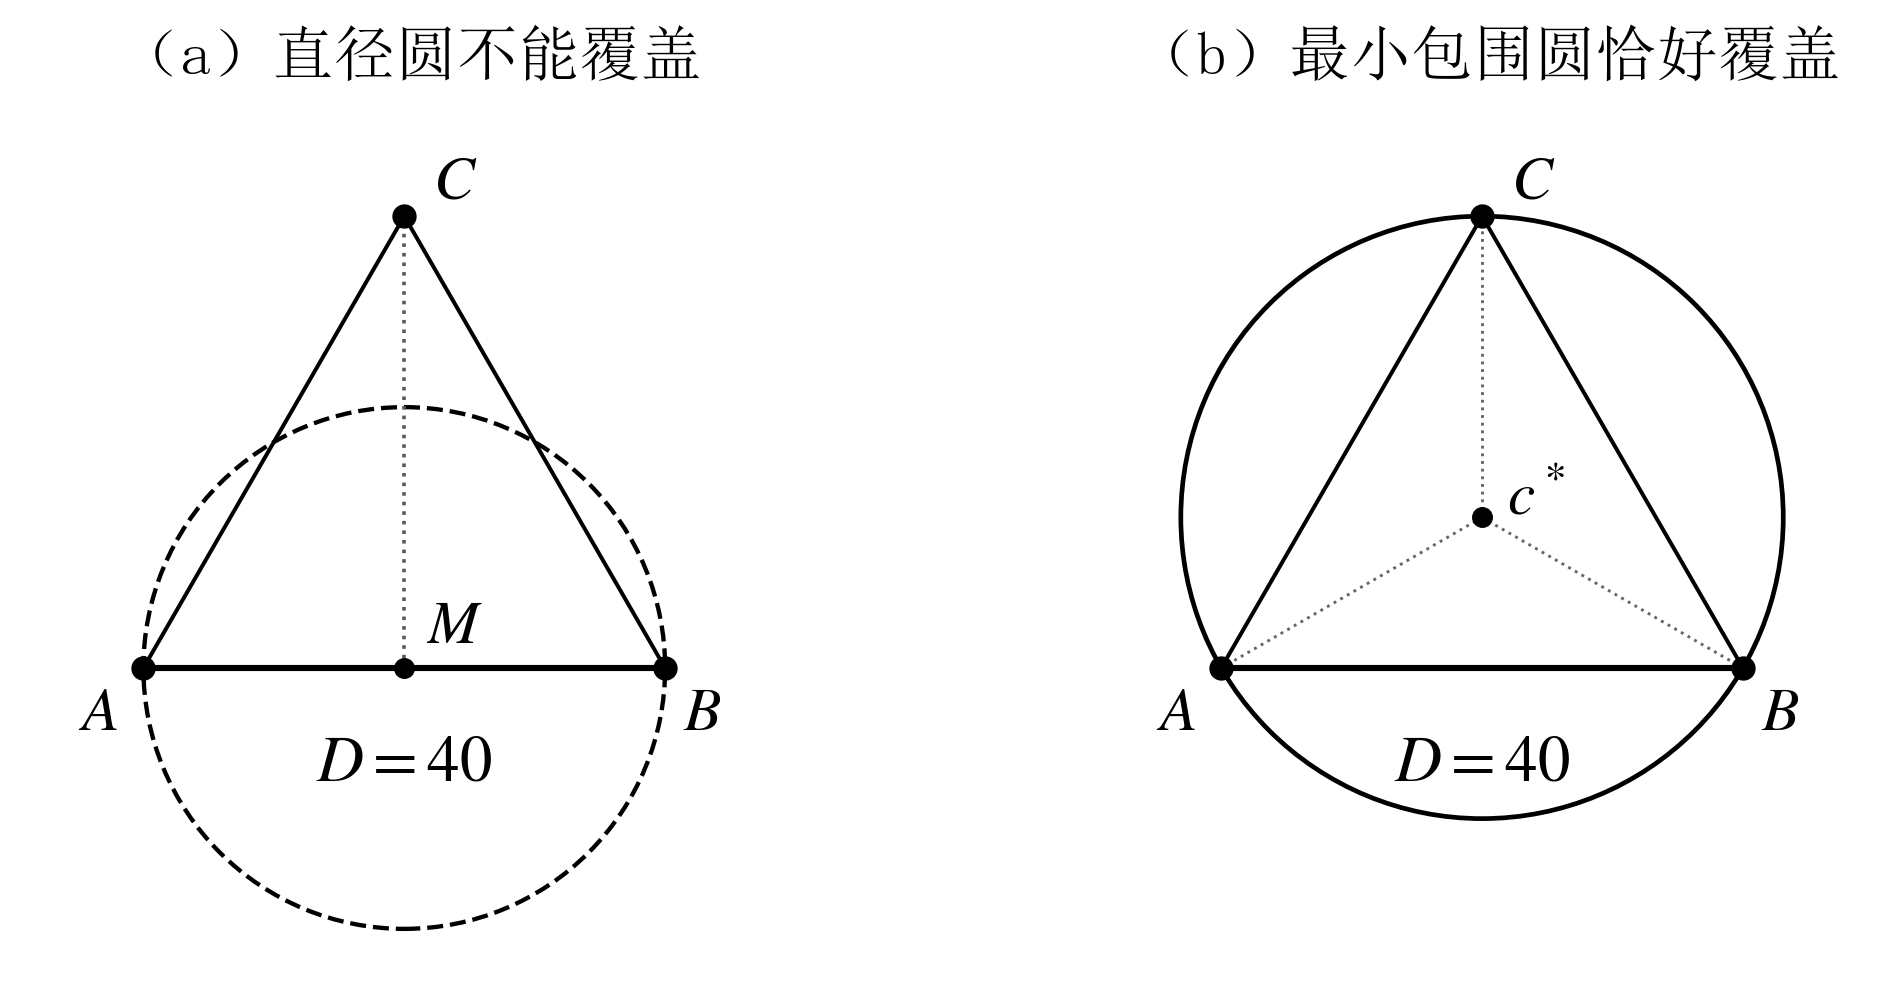
\includegraphics[width=0.84\linewidth,height=0.68\textheight,keepaspectratio]{figures/q1_cover_bw.png}
\caption{等边三角形的直径圆与最小包围圆（长度单位：米）}\label{fig:old1}
\end{figure}

如图\ref{fig:old1} 所示，故以定位区域直径为直径的圆不一定覆盖定位区域。

\subsection{算法准确性与鲁棒性验证}

为检验算法输出的准确性与鲁棒性，我们预先给定干扰源真值 \(G\)，由 \(G\) 与检测点坐标反算真实方向，再按题设误差界生成示向度，构造出定位结果已知的算例。

实例选取四种代表性有界构型：以等边三角形代表一般多边形形态、以线段与单点代表退化形态、以薄多边形代表近退化情形。各实例的构造参数、检测点坐标与示向度如表\ref{tab:old3} 所示。

\begingroup
\renewcommand{\baselinestretch}{1.10}\fontsize{9}{11.5}\selectfont
\setlength{\LTpost}{3pt}
\setlength{\tabcolsep}{4pt}
\setlength{\TableInnerWidth}{\dimexpr\linewidth-6\tabcolsep\relax}
\renewcommand{\arraystretch}{1.05}
\begin{longtable}{@{}>{\centering\arraybackslash}p{0.350\TableInnerWidth}>{\centering\arraybackslash}p{0.340\TableInnerWidth}>{\centering\arraybackslash}p{0.120\TableInnerWidth}>{\centering\arraybackslash}p{0.190\TableInnerWidth}@{}}
\caption{四类实例的构造参数、检测点与示向度}\label{tab:old3}\\
\toprule
实例与构造参数 & 检测点坐标 \(S_i=(x_i,y_i)\) / 米 & 示向度 \(\theta_i\) / ° & 相对真值误差 \(\varepsilon_i\) / ° \\
\midrule
\endfirsthead
\multicolumn{4}{c}{表\thetable\quad 四类实例的构造参数、检测点与示向度（续）}\\
\toprule
实例与构造参数 & 检测点坐标 \(S_i=(x_i,y_i)\) / 米 & 示向度 \(\theta_i\) / ° & 相对真值误差 \(\varepsilon_i\) / ° \\
\midrule
\endhead
\midrule
\multicolumn{4}{r}{续下页}\\
\endfoot
\bottomrule
\endlastfoot
{(a) 三角形　真值 \(G=(0,0)\)；参考圆 \(r=20\) 米；边长 \(20\sqrt3\) 米；测站基距 \(L=1200\) 米} & \parbox[t]{\linewidth}{\centering\setlength{\baselineskip}{14pt}
\rule[-3pt]{0pt}{14pt}\((-1200,-10)\) \\
\rule[-3pt]{0pt}{14pt}\((600+5\sqrt3,\,-600\sqrt3+5)\) \\
\rule[-3pt]{0pt}{14pt}\((600-5\sqrt3,\,600\sqrt3+5)\)
} & \parbox[t]{\linewidth}{\centering\setlength{\baselineskip}{14pt}
\rule[-3pt]{0pt}{14pt}1 \\
\rule[-3pt]{0pt}{14pt}121 \\
\rule[-3pt]{0pt}{14pt}241
} & \parbox[t]{\linewidth}{\centering\setlength{\baselineskip}{14pt}
\rule[-3pt]{0pt}{14pt}+0.522546 \\
\rule[-3pt]{0pt}{14pt}+0.522546 \\
\rule[-3pt]{0pt}{14pt}+0.522546
} \\
\midrule
{(b) 线段　真值 \(G=(50,0)\)；端点 \((0,0)\)、\((100,0)\)；长度 \(100\) 米；参考圆 \(r=50\) 米} & \parbox[t]{\linewidth}{\centering\setlength{\baselineskip}{14pt}
\rule[-3pt]{0pt}{14pt}\((0,0)\) \\
\rule[-3pt]{0pt}{14pt}\((100,0)\)
} & \parbox[t]{\linewidth}{\centering\setlength{\baselineskip}{14pt}
\rule[-3pt]{0pt}{14pt}1 \\
\rule[-3pt]{0pt}{14pt}181
} & \parbox[t]{\linewidth}{\centering\setlength{\baselineskip}{14pt}
\rule[-3pt]{0pt}{14pt}+1.000000 \\
\rule[-3pt]{0pt}{14pt}+1.000000
} \\
\midrule
{(c) 单点　真值 \(G=(0,0)\)；参考圆 \(r=0\)；测站基距 \(L=100\) 米} & \parbox[t]{\linewidth}{\centering\setlength{\baselineskip}{14pt}
\rule[-3pt]{0pt}{14pt}\((-100,0)\) \\
\rule[-3pt]{0pt}{14pt}\((50,-50\sqrt3)\) \\
\rule[-3pt]{0pt}{14pt}\((50,50\sqrt3)\)
} & \parbox[t]{\linewidth}{\centering\setlength{\baselineskip}{14pt}
\rule[-3pt]{0pt}{14pt}1 \\
\rule[-3pt]{0pt}{14pt}121 \\
\rule[-3pt]{0pt}{14pt}241
} & \parbox[t]{\linewidth}{\centering\setlength{\baselineskip}{14pt}
\rule[-3pt]{0pt}{14pt}+1.000000 \\
\rule[-3pt]{0pt}{14pt}+1.000000 \\
\rule[-3pt]{0pt}{14pt}+1.000000
} \\
\midrule
{(d) 薄多边形　真值 \(G=(50,0.0005)\)；高度 \(h=0.001\) 米；对角线横向跨度 \(100\) 米} & \parbox[t]{\linewidth}{\centering\setlength{\baselineskip}{14pt}
\rule[-3pt]{0pt}{14pt}\((0,0)\) \\
\rule[-3pt]{0pt}{14pt}\((100,0.001)\)
} & \parbox[t]{\linewidth}{\centering\setlength{\baselineskip}{14pt}
\rule[-3pt]{0pt}{14pt}1 \\
\rule[-3pt]{0pt}{14pt}181
} & \parbox[t]{\linewidth}{\centering\setlength{\baselineskip}{14pt}
\rule[-3pt]{0pt}{14pt}+0.999427 \\
\rule[-3pt]{0pt}{14pt}+0.999427
} \\
\end{longtable}
\endgroup

\begingroup\renewcommand{\baselinestretch}{1.10}\fontsize{8.5}{11}\selectfont\noindent 注：示向度\(\theta_i\)的取值规则为\(\theta_i=\beta_i+\varepsilon_i\)，其中设检测点 \(S_i\) 指向预设真值 \(G\) 的真实方向为 \(\beta_i\)。\par\endgroup

\begin{figure}[H]
\centering
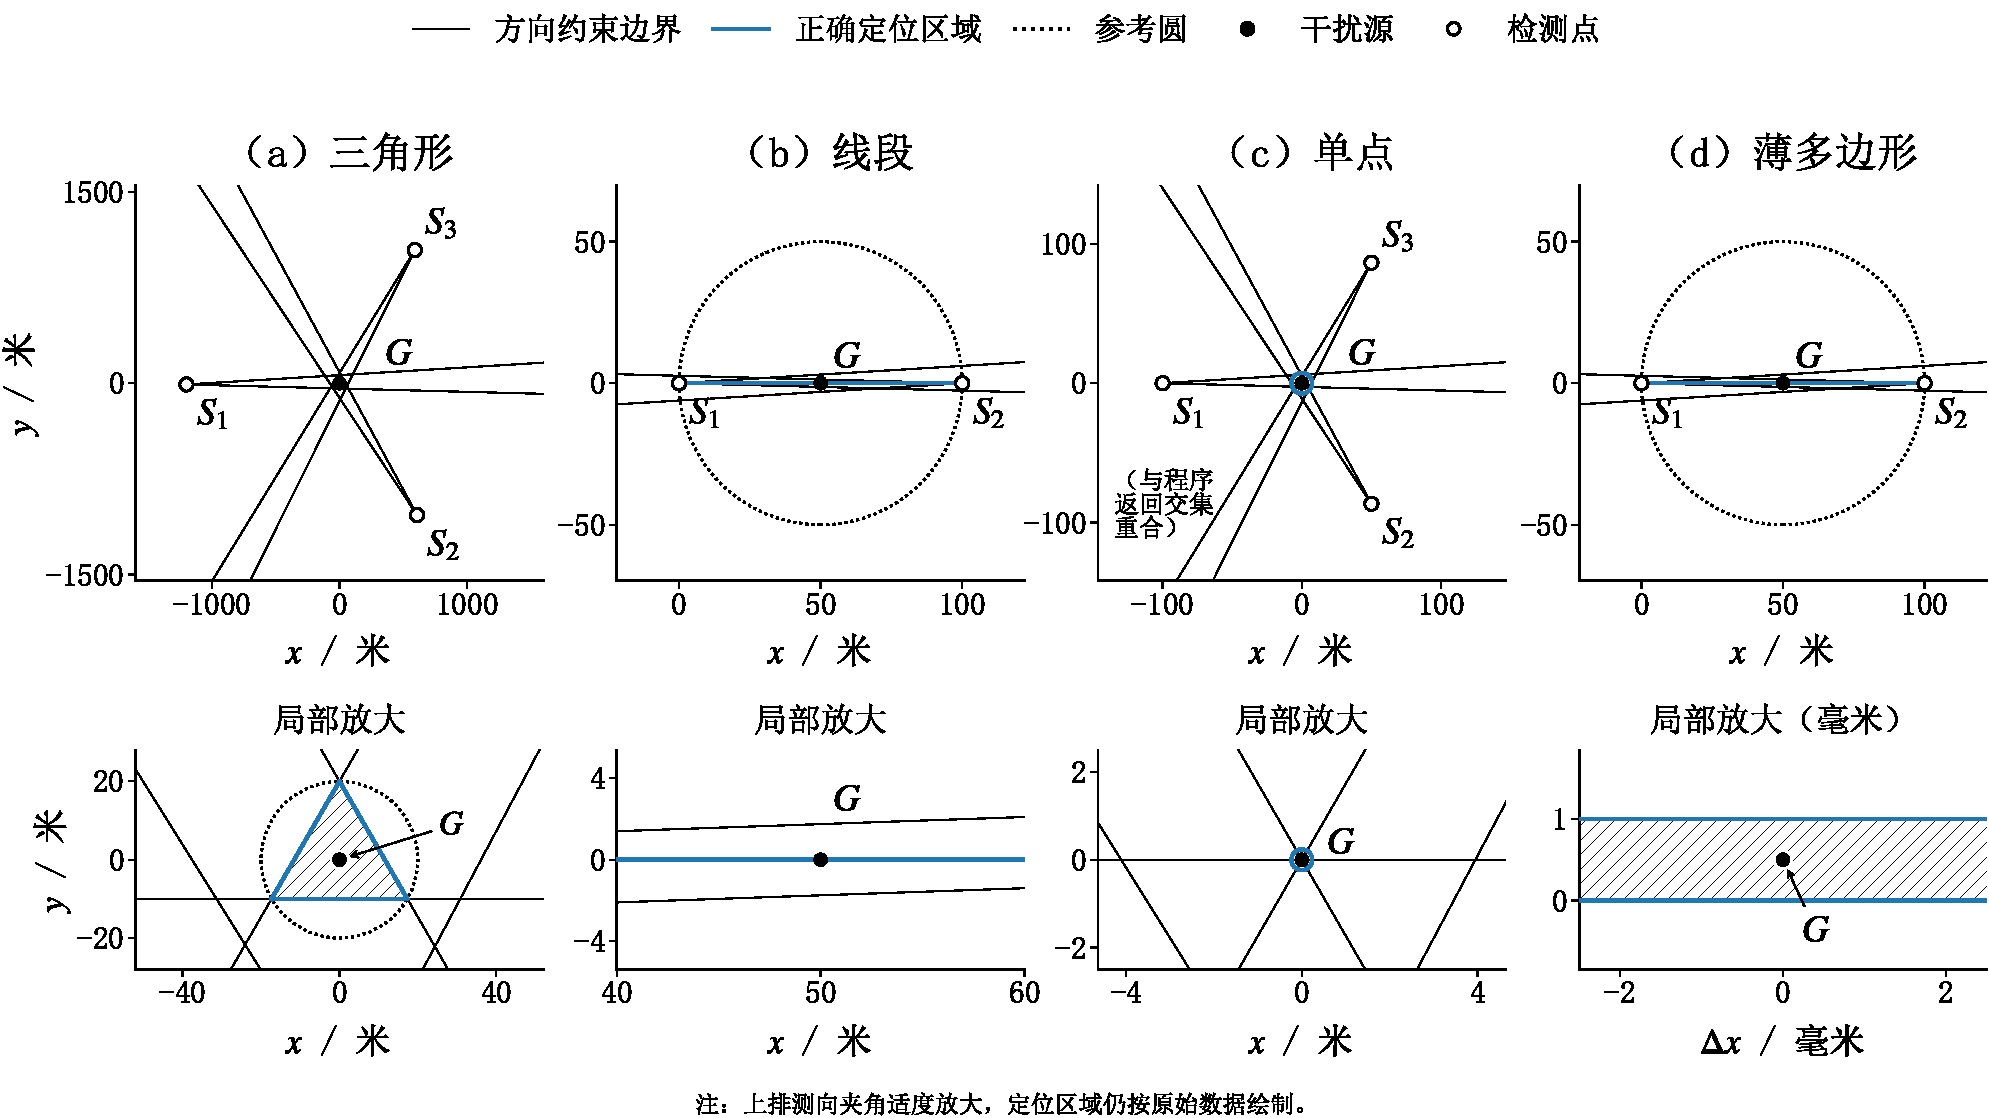
\includegraphics[width=1.00\linewidth,height=0.68\textheight,keepaspectratio]{figures/q1_cases_bw.pdf}
\caption{四类实例的检测点分布与程序返回的定位区域}\label{fig:old2}
\end{figure}

如图\ref{fig:old2}，对每个实例，我们将程序返回的区域类型与顶点集合同预设区域逐一比对，结果发现四类实例在既定数值容差下均与预设区域一致，且预设真值均落入程序返回的定位区域，共同证明了算法具有优秀的准确性与鲁棒性。

\FloatBarrier
\section{问题二的模型建立与求解}

\subsection{定位区域}

\subsubsection{首次观测的定位区域}

主动测向定位通过选择后续检测位置改善目标估计\textsuperscript{\cite{ref2}}。本问对一个全向干扰源定位，接收半径 \(R\) 固定未知且满足 \(1000\le R\le1500\) 米。我们在第一问的基础上引入距离约束，将满足目标范围、角度、距离与已有反馈约束的源位置集合称为定位区域。记：
\[
d_s(g)=\|g-s\|_2, \qquad d_1(g)=\|g-s_1\|_2
\]

由题意知，首次反馈信号为示向度，故目标既满足角度误差界，同时位于 5 米以内的近距离反馈范围之外和接收范围内。故位置与接收半径的联合可行集为：
\[
\mathcal X_1=
\left\{(g,R):
g\in\Omega\cap W(s_1,\theta_1),
\,
5<d_1(g)\le R,\,1000\le R\le1500
\right\}
\tag{8}
\]

化简可得：
\[
F_1=\Omega\cap W(s_1,\theta_1)\cap\{g:5<d_1(g)\le1500\},
\,
R\mid g\in[\max\{1000,d_1(g)\},1500]
\tag{9}
\]

其中，\(R\mid g\) 表示给定干扰源位置后的半径允许范围。

\subsubsection{二次观测的定位区域更新}

第二检测点确定后，可能得到近距离、返回方向或无信号三类反馈。为统一描述这一过程，我们仍以式（8）中的联合状态为基本对象：
\[
x=(g,R)\in\mathcal X_1
\]

其中，\(g\) 为干扰源位置，\(R\) 为该干扰源固定但未知的有效接收半径。对给定状态 \(x=(g,R)\) 和第二检测点 \(s\)，我们定义该状态可能产生的反馈集合：
\[
\mathcal H(x,s)=
\begin{cases}
\{\text{near}\},&d_s(g)\le5,\\[2mm]
\{\text{direction}(\beta):\beta\in\Gamma(s,g)\},&5<d_s(g)\le R,\\[2mm]
\{\text{no-signal}\},&d_s(g)>R
\end{cases}
\tag{10}
\]

其中，\(\Gamma(s,g)\) 表示位置 \(g\) 在检测点 \(s\) 处可能产生的示向度读数集合。由题意，同一地点、同一频道的测向误差固定，故：
\[
\Gamma(s,g)=
\begin{cases}
\{\theta_1\},&s=s_1,\\[2mm]
\{\beta\in[0^\circ,360^\circ):g\in W(s,\beta)\},&s\ne s_1
\end{cases}
\tag{11}
\]

我们遍历首次观测后的全部可行状态，得到检测点 \(s\) 处可能出现的反馈集合\(\mathcal Y(s)=\bigcup_{x\in\mathcal X_1}\mathcal H(x,s).\)在检测点 \(s\) 实际得到反馈 \(y\in\mathcal Y(s)\) 时，我们保留所有能够产生该反馈的联合状态，定义：
\[
\mathcal X_2(s,y)
=\{x\in\mathcal X_1:y\in\mathcal H(x,s)\}
\tag{12}
\]

下面分别讨论三类反馈得到的新定位区域形式。

\textbf{（1）返回near}

近距离反馈等价于 \(d_s(g)\le5\)。由于 \(R\ge1000>5\)，满足该条件的全向干扰源必然位于接收范围内，因而：
\[
F_n(s)
=\operatorname{proj}_g\mathcal X_2(s,\text{近距离})
=F_1\cap\{g:d_s(g)\le5\}
\tag{13a}
\]

其中，首次返回方向已经给出 \(d_1(g)>5\)，故 \(F_n(s_1)=\varnothing\)，原地重复检测不产生近距离反馈。

\textbf{（2）返回方向 \(\beta\)}

当\(s=s_1\)时，定位区域不变；当 \(s\ne s_1\) 时，定位区域更新为首次定位区域与二次定位区域的交，即：
\[
\begin{aligned}
F_d(s,\beta)
&=\operatorname{proj}_g\mathcal X_2(s,\text{方向}(\beta))\\
&=\begin{cases}
F_1,&s=s_1,\ \beta=\theta_1\\[1mm]
F_1\cap W(s,\beta)\cap\{g:5<d_s(g)\le1500\},&s\ne s_1
\end{cases}
\end{aligned}
\tag{13b}
\]

\textbf{（3）返回no-signal}

无信号反馈对应第二检测点位于实际接收半径之外的情形。于是：
\[
\begin{aligned}
F_0(s)
&=\operatorname{proj}_g\mathcal X_2(s,\text{无信号})\\
&=F_1\cap\{g:d_s(g)>\max\{1000,d_1(g)\}\}\\
&=F_1\cap\{g:d_s(g)>1000\}\cap\{g:d_s(g)>d_1(g)\}
\end{aligned}
\tag{13c}
\]

式（13c）反映了目标位于以 \(s\) 为圆心的 1000 米圆外即\(\|g-s\|_2 > 1000\)；目标到第二检测点的距离大于到首次检测点的距离，即以两检测点连线的垂直平分线为边界、取到第二检测点更远一侧的开半平面，因此后一条件等价于：
\[
d_s(g)>d_1(g)
\quad\Longleftrightarrow\quad
2g^{\mathsf T}(s-s_1)<\|s\|_2^2-\|s_1\|_2^2,
\]

其中，当 \(s=s_1\) 时，\(d_s(g)=d_1(g)\)，故 \(F_0(s_1)=\varnothing\)。接收边界属于有信号一侧，式（13c）保留严格不等号；在判定反馈集合非空之后，计算最小包围圆半径时取闭包。

综合以上三种情况，在第二检测点得到反馈 \(y\) 对应的定位区域可统一记为：
\[
F_2(s,y)
=\operatorname{proj}_g\mathcal X_2(s,y)
=
\begin{cases}
F_n(s),&y=\text{近距离},\\
F_d(s,\beta),&y=\text{方向}(\beta),\\
F_0(s),&y=\text{无信号}
\end{cases}
\tag{14}
\]

三类反馈的定位区域更新情况如图\ref{fig:old3} 所示

\begin{figure}[H]
\centering
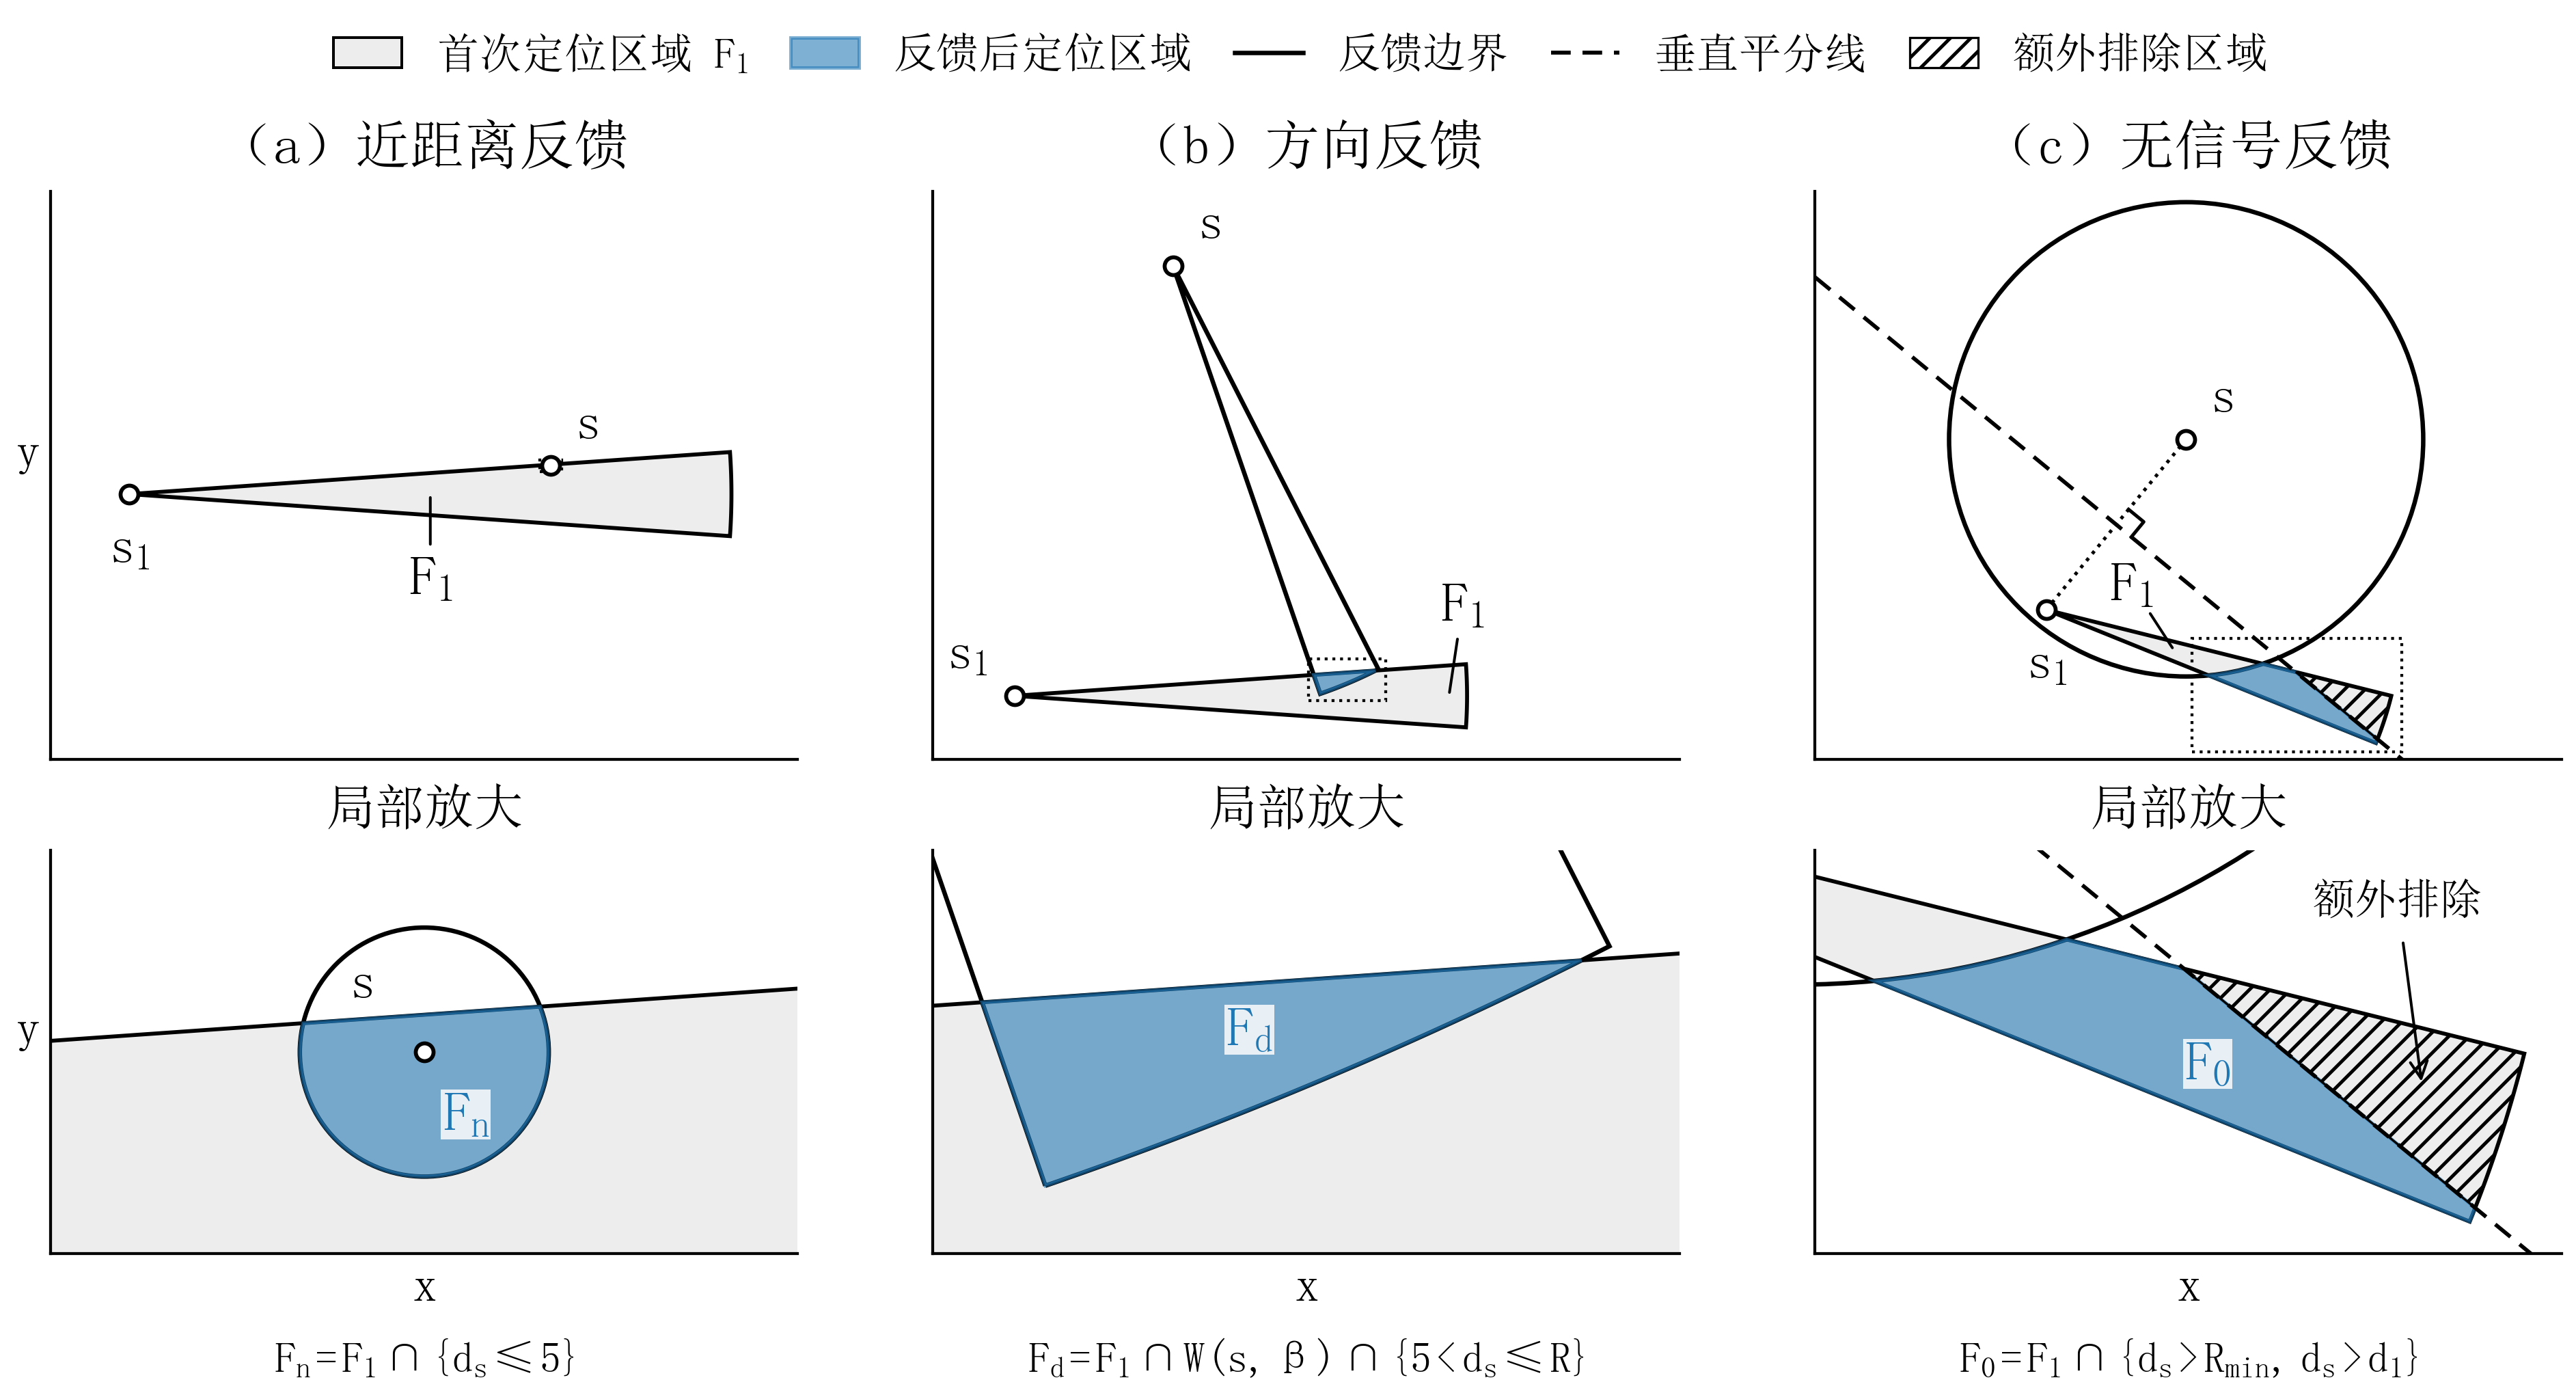
\includegraphics[width=0.96\linewidth,height=0.68\textheight,keepaspectratio]{figures/q2_three_feedback_schematic.png}
\caption{三类反馈下的定位区域更新}\label{fig:old3}
\end{figure}

\subsection{最小包围圆半径与定位损失}

\subsubsection{定位效果指标的选定}

纯方位观测中的几何布局会影响可观测性与定位精度\textsuperscript{\cite{ref3,ref5}}。本问在反馈之后交付干扰源预测位置，由于干扰源位置一定在定位区域内，故评价标准是预测位置到定位区域内点的最大距离。评价指标须同时给出预测位置的几何中心与误差上界，但问题一所用的区域直径 \(D(P)\) 只刻画角度交会区域的跨度，而本问所需的两项指标由最小包围圆一并给出，所以我们据此替换评价指标。

对非空有界的定位区域 \(F\)，我们选取最坏误差最小的点作为预测位置，以该最小最坏误差作为误差上界：
\[
\hat g(F)\in\arg\min_{c\in\mathbb R^2}\sup_{g\in F}\|g-c\|_2
\,,\qquad
\rho(F)=\min_{c\in\mathbb R^2}\sup_{g\in F}\|g-c\|_2
\tag{15}
\]

其中，\(\hat g(F)\) 为反馈后的预测位置，\(\rho(F)\) 为定位区域 \(F\) 的最小包围圆半径。式（15）表明，\(\hat g(F)\) 为全部预测点中最优的一个，\(\rho(F)\) 为该位置在全部相容位置上的最坏误差，即本次定位在最优预测下达到的误差上界。

该指标的优势在于：可区分直径相同而形状不同的定位区域；与题干第三问20米的光学精确定位距离直接对应：半径不超过20米时，圆心即可作为进入光学作业范围的预测位置。

\subsubsection{最坏定位误差}

由式（15），\(\hat g(F_2(s,y))\) 给出反馈 \(y\) 后的预测位置，\(\rho(F_2(s,y))\) 给出该预测在全部相容位置上的最坏误差。

对于给定的第二检测点 \(s\) 和实际反馈 \(y\)，我们定义单次反馈下的定位损失 \(L(s,y)\) 为该反馈下更新区域能够达到的最小最坏预测误差：
\[
L(s,y)=\rho\bigl(F_2(s,y)\bigr)
\tag{16}
\]

考虑到选择第二检测点时实际反馈尚未发生，此时反馈的可能范围为 \(y\in\mathcal Y(s)\)。我们对检测点 \(s\) 的全部可能反馈取最坏值，定义``最坏反馈定位损失''：
\[
J(s)=\sup_{y\in\mathcal Y(s)}L(s,y)
=\sup_{y\in\mathcal Y(s)}\rho\bigl(F_2(s,y)\bigr)
\tag{17}
\]

为显式展示三类反馈在式（17）中的作用，记检测点 \(s\) 处所有可能返回的方向读数为 \(\mathcal B(s)=\{\beta\in[0^\circ,360^\circ):F_d(s,\beta)\ne\varnothing\}\)，则式（17）等价于：
\[
J(s)=\sup\Bigl(\{\rho(F_d(s,\beta)):\beta\in\mathcal B(s)\}\cup\{\rho(F_k(s)):k\in\{n,0\},\ F_k(s)\ne\varnothing\}\Bigr)
\]

其中，\(k\in\{n,0\}\) 分别对应近距离与无信号反馈。

\(J(s)\) 越小，剩余位置集合在每一种相容反馈下都能由越小的圆覆盖，该检测点的最坏定位效果越好。

\subsection{第二检测点的候选区域与选点策略}

\subsubsection{第二检测点的候选区域}

第二检测点在平面上取任意位置；距离首次定位区域过远的检测点只产生可预先确定的无信号反馈，不提供新的定位信息。记点到集合的距离为：
\[
\operatorname{dist}(s,A)=\inf_{g\in A}\|s-g\|_2,
\]

我们将第二检测点的候选区域确定为：
\[
\mathcal S=
\{s:\operatorname{dist}(s,\overline{F_1})\le1500\}
\tag{18}
\]

对 \(s\notin\mathcal S\) 与任意 \(g\in F_1\) 均有 \(d_s(g)>1500\)，同时有效接收半径满足 \(R\le1500\)，故此时第二次检测必然无信号。故 \(\mathcal S\) 包含全部可能产生信息增益的检测位置，把无限平面上的选点问题限制在此有限候选区域内。

\subsubsection{基于最坏定位误差的第二检测点选址模型}

由式（17），每个检测点 \(s\in\mathcal S\) 对应最坏反馈定位损失为 \(J(s)\)。记搜索域内的最优损失为 \(J^*\)，我们定义``最优二次检测点''：
\[
J^*=\min_{s\in\mathcal S}J(s),\qquad s^*\in\arg\min_{s\in\mathcal S}J(s)
\tag{19}
\]

该检测点具有``最坏情形最优''的数学特点：在所有候选位置中，它使最不利反馈对应的定位损失达到最小。以反馈后定位区域的最小包围圆圆心预测时，任一相容反馈下的预测误差均不超过 \(J^*\)，且其他检测位置无法提供更小的统一误差上界，因此该点具有针对反馈不确定性的最优误差保障。

\subsection{最优二次检测点的求解}

上述模型包含位置搜索、方向反馈枚举及曲边区域求交。我们采用``粗网格与局部增密搜索算法''，对各候选点统一计算三类反馈后的最小包围圆半径，并据此提取近优候选集。

\textbf{Step 1　构造首次定位区域。} 输入第一次检测位置 \(s_1\)、示向度 \(\theta_1\) 及题设常量，按式（9）构造首次定位区域 \(F_1\)，并保留位置与有效接收半径之间的对应关系。若 \(F_1=\varnothing\)，则判定观测结果不相容。

\textbf{Step 2　离散第二检测点候选区域。} 式（18）给出的候选区域为连续集合，无法逐点计算，因此先以100米为间距生成位置网格，并将网格点作为第二检测点的有限候选。

\textbf{Step 3　计算最坏定位损失。} 对每个候选位置 \(s\)，构造三类反馈对应的定位区域并计算其最小包围圆半径，取所有可能反馈下的最大半径作为该位置的最坏定位损失 \(\widehat J(s)\)。

\textbf{Step 4　逐级增密位置网格迭代最优位置。} 比较各网格点的 \(\widehat J(s)\)，在损失较小的区域依次将网格间距缩小为20米、2米和0.5米，并重复Step 3，得到更精确的第二检测位置。

以首次检测点为原点、示向度为\(0^\circ\)为例，数值搜索结果如图\ref{fig:q2-station-search}所示，算法伪代码见附录B。

\begin{figure}[H]
\centering
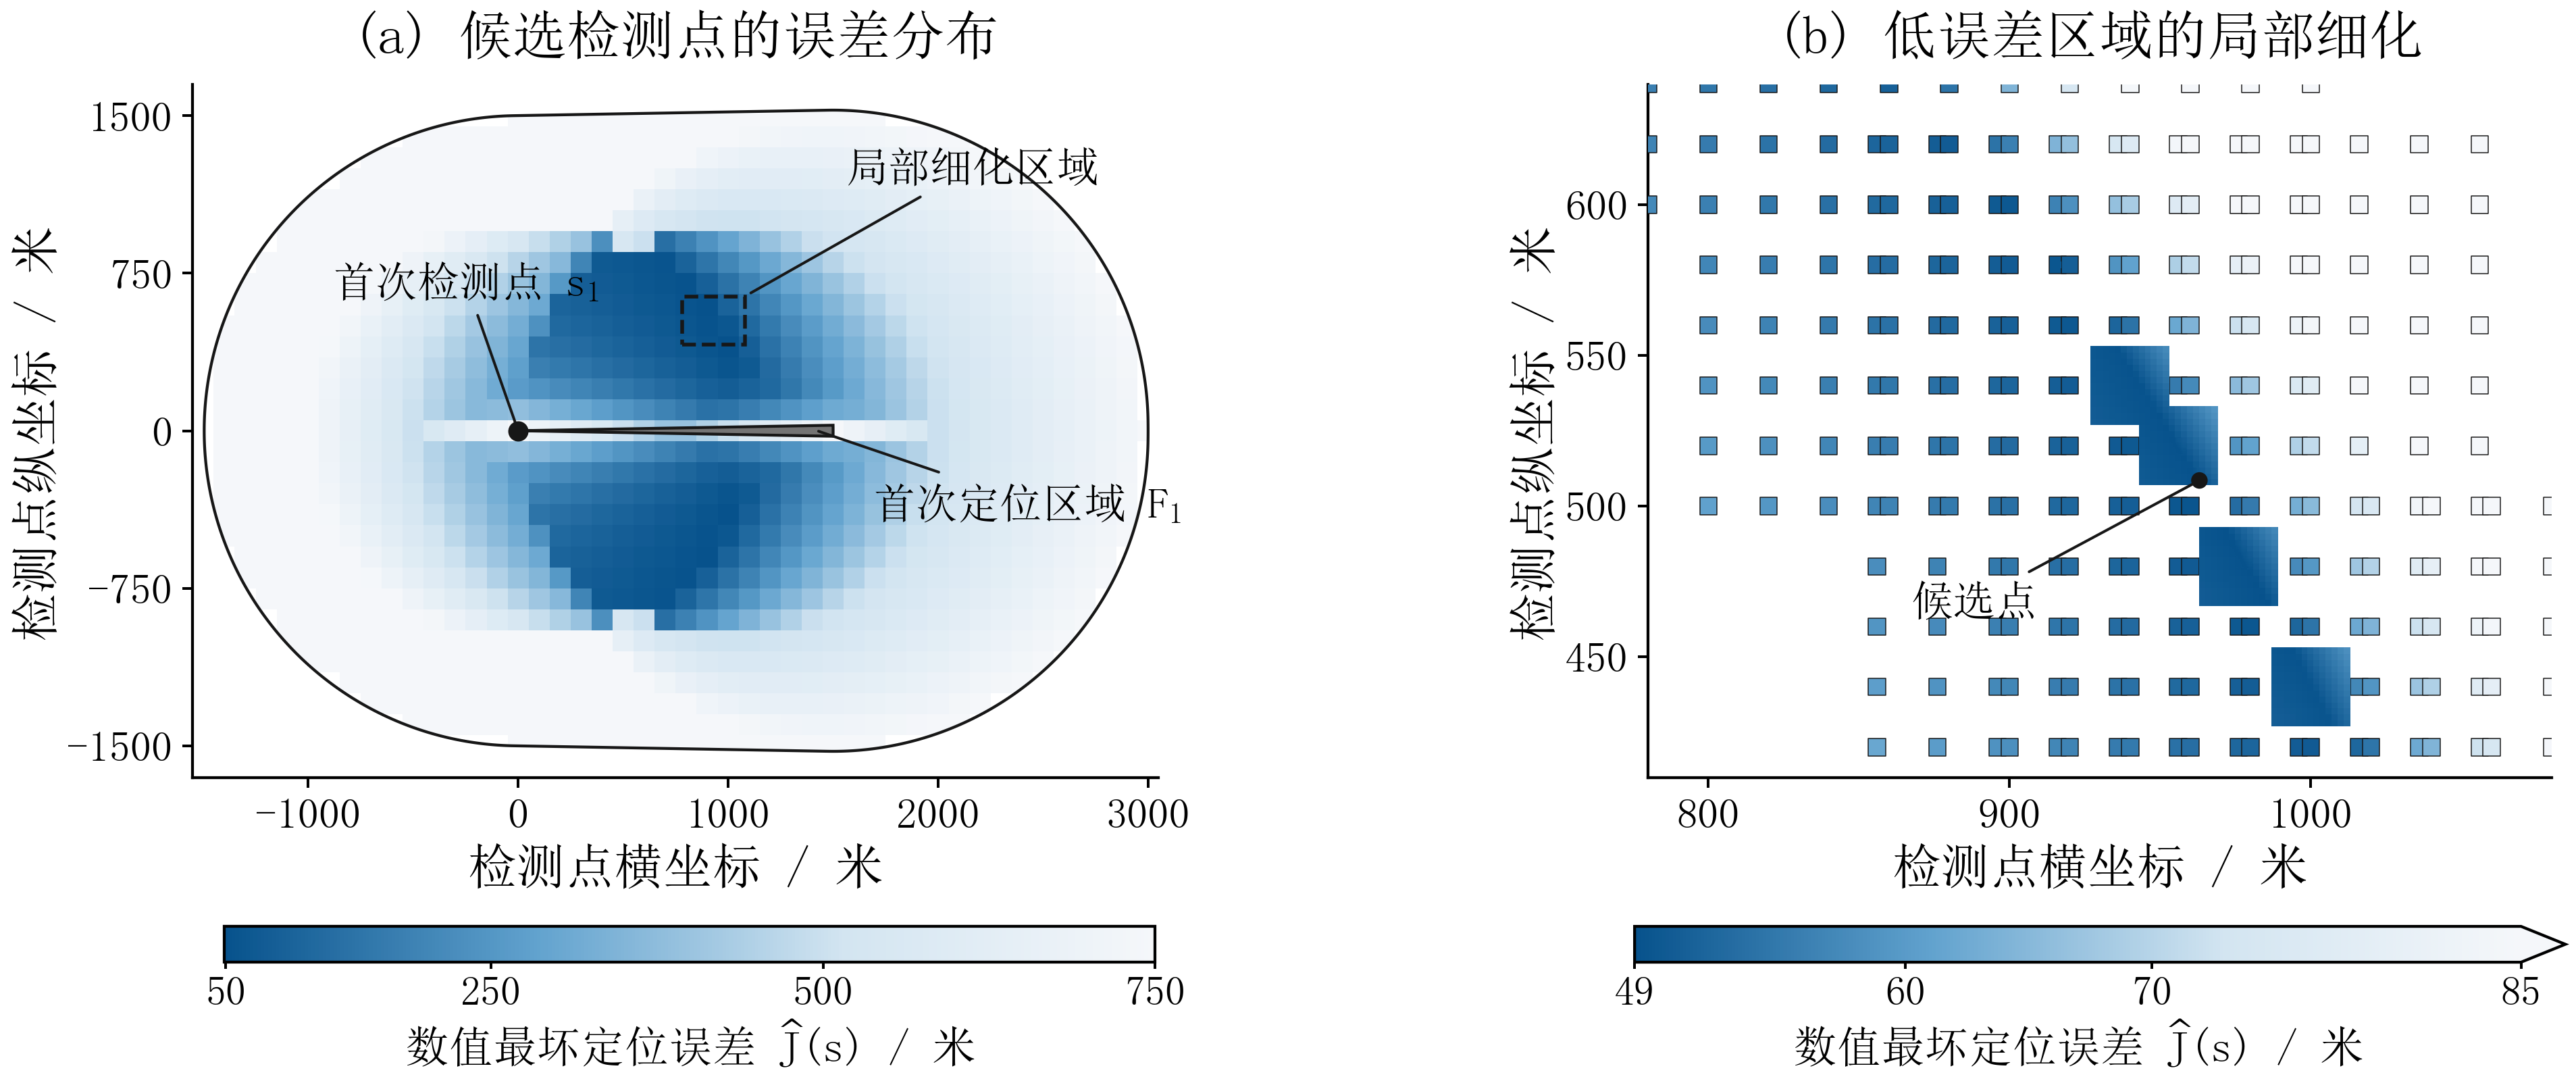
\includegraphics[width=\linewidth]{figures/q2_station_search.png}
\caption{候选检测点的最坏定位误差分布与局部细化}\label{fig:q2-station-search}
\end{figure}

\subsection{预测精度与选点作用检验}

我们以预测位置与真实位置的距离为依据，开展配对模拟实验，分别检验新增观测与检测点选择对定位精度的影响。

\subsubsection{测试设置与评价指标}

按演练生成规则构造模拟场景，源中心在目标圆域内留有30米边界余量，其余参数按演练分布抽样，测向误差采用按频道区分的固定平滑误差场。选取首次在原点获得方向反馈的5000例，三条规则在相同场景与首次观测下开展配对测试。

记规则 \(\pi\) 的预测位置为 \(\hat g_\pi\)、首次反馈为 \(Y_1\)，定义条件均方误差及均方根误差：
\[
\mathcal R(\pi;s_1)
=\mathbb E\!\left[
\|\hat g_\pi-g\|_2^2
\mid Y_1=\text{方向},s_1
\right],
\qquad
\mathcal E(\pi;s_1)=\sqrt{\mathcal R(\pi;s_1)}
\]

对 \(N=5000\) 个样本，令 \(e_i=\|\hat g_i-g_i\|_2\)，以样本均方根误差评价整体定位精度：
\[
\widehat{\mathcal E}
=\sqrt{\frac1N\sum_{i=1}^{N}e_i^2}
\]

该指标以米为单位，数值越小，整体定位精度越高。

\subsubsection{选点规则与预测结果}

我们设置表\ref{tab:old4}所示的三条规则。比较``仅用首次观测''与``随机选取第二点''，检验新增观测的作用；比较两条二次检测规则，检验相同观测次数下的选点优化效果。

\begingroup
\small
\setlength{\tabcolsep}{4pt}
\setlength{\TableInnerWidth}{\dimexpr\linewidth-4\tabcolsep\relax}
\renewcommand{\arraystretch}{1.22}
\begin{longtable}{@{}>{\centering\arraybackslash}p{0.250\TableInnerWidth}>{\centering\arraybackslash}p{0.120\TableInnerWidth}>{\centering\arraybackslash}p{0.630\TableInnerWidth}@{}}
\caption{观测与选点规则}\label{tab:old4}\\
\toprule
规则 & 观测次数 & 第二点选择 \\
\midrule
\endfirsthead
\multicolumn{3}{c}{表\thetable\quad 观测与选点规则（续）}\\
\toprule
规则 & 观测次数 & 第二点选择 \\
\midrule
\endhead
\midrule
\multicolumn{3}{r}{续下页}\\
\endfoot
\bottomrule
\endlastfoot
仅用首次观测 & 1 & 不增加第二次观测 \\
随机选取第二点 & 2 & 在式（18）的搜索外包域内按面积均匀抽样，每例抽取一次 \\
本文选点规则 & 2 & 按首次示向度旋转预先求得的代表点 \\
\end{longtable}
\endgroup

三条规则均采用最小包围圆圆心预测源位置。其中，仅用首次观测时，以 \(\hat g(F_1)\) 作为预测位置；采用两次观测时，两条规则使用相同的反馈更新与位置估计方法。

三条规则在同批5000例上的预测误差如表\ref{tab:old5}所示。

\begingroup
\small
\setlength{\tabcolsep}{4pt}
\setlength{\TableInnerWidth}{\dimexpr\linewidth-8\tabcolsep\relax}
\renewcommand{\arraystretch}{1.22}
\begin{longtable}{@{}>{\centering\arraybackslash}p{0.250\TableInnerWidth}>{\centering\arraybackslash}p{0.190\TableInnerWidth}>{\centering\arraybackslash}p{0.200\TableInnerWidth}>{\centering\arraybackslash}p{0.160\TableInnerWidth}>{\centering\arraybackslash}p{0.200\TableInnerWidth}@{}}
\caption{同批5000例的预测误差}\label{tab:old5}\\
\toprule
规则 & 均方根误差 / 米 & 平均距离误差 / 米 & 中位数 / 米 & 95\%分位数 / 米 \\
\midrule
\endfirsthead
\multicolumn{5}{c}{表\thetable\quad 同批5000例的预测误差（续）}\\
\toprule
规则 & 均方根误差 / 米 & 平均距离误差 / 米 & 中位数 / 米 & 95\%分位数 / 米 \\
\midrule
\endhead
\midrule
\multicolumn{5}{r}{续下页}\\
\endfoot
\bottomrule
\endlastfoot
仅用首次观测 & 333.828 & 281.789 & 263.149 & 610.216 \\
随机选取第二点 & 229.057 & 151.509 & 66.078 & 512.487 \\
本文选点规则 & 12.091 & 10.543 & 9.611 & 21.444 \\
\end{longtable}
\endgroup

由表\ref{tab:old5}，随机增加一次观测使均方根误差由333.828米降至229.057米；在同为两次观测的条件下，本文规则进一步降至12.091米，较随机选点减少216.965米。上述结果表明，在该测试分布下，本文选点规则仅需两次观测即可达到10米级的整体定位精度，体现了检测点优化在有限观测条件下的定位优势。

三条规则的预测误差累积分布如图\ref{fig:q2-error-ecdf}所示，右图进一步放大小误差区间。

\begin{figure}[H]
\centering
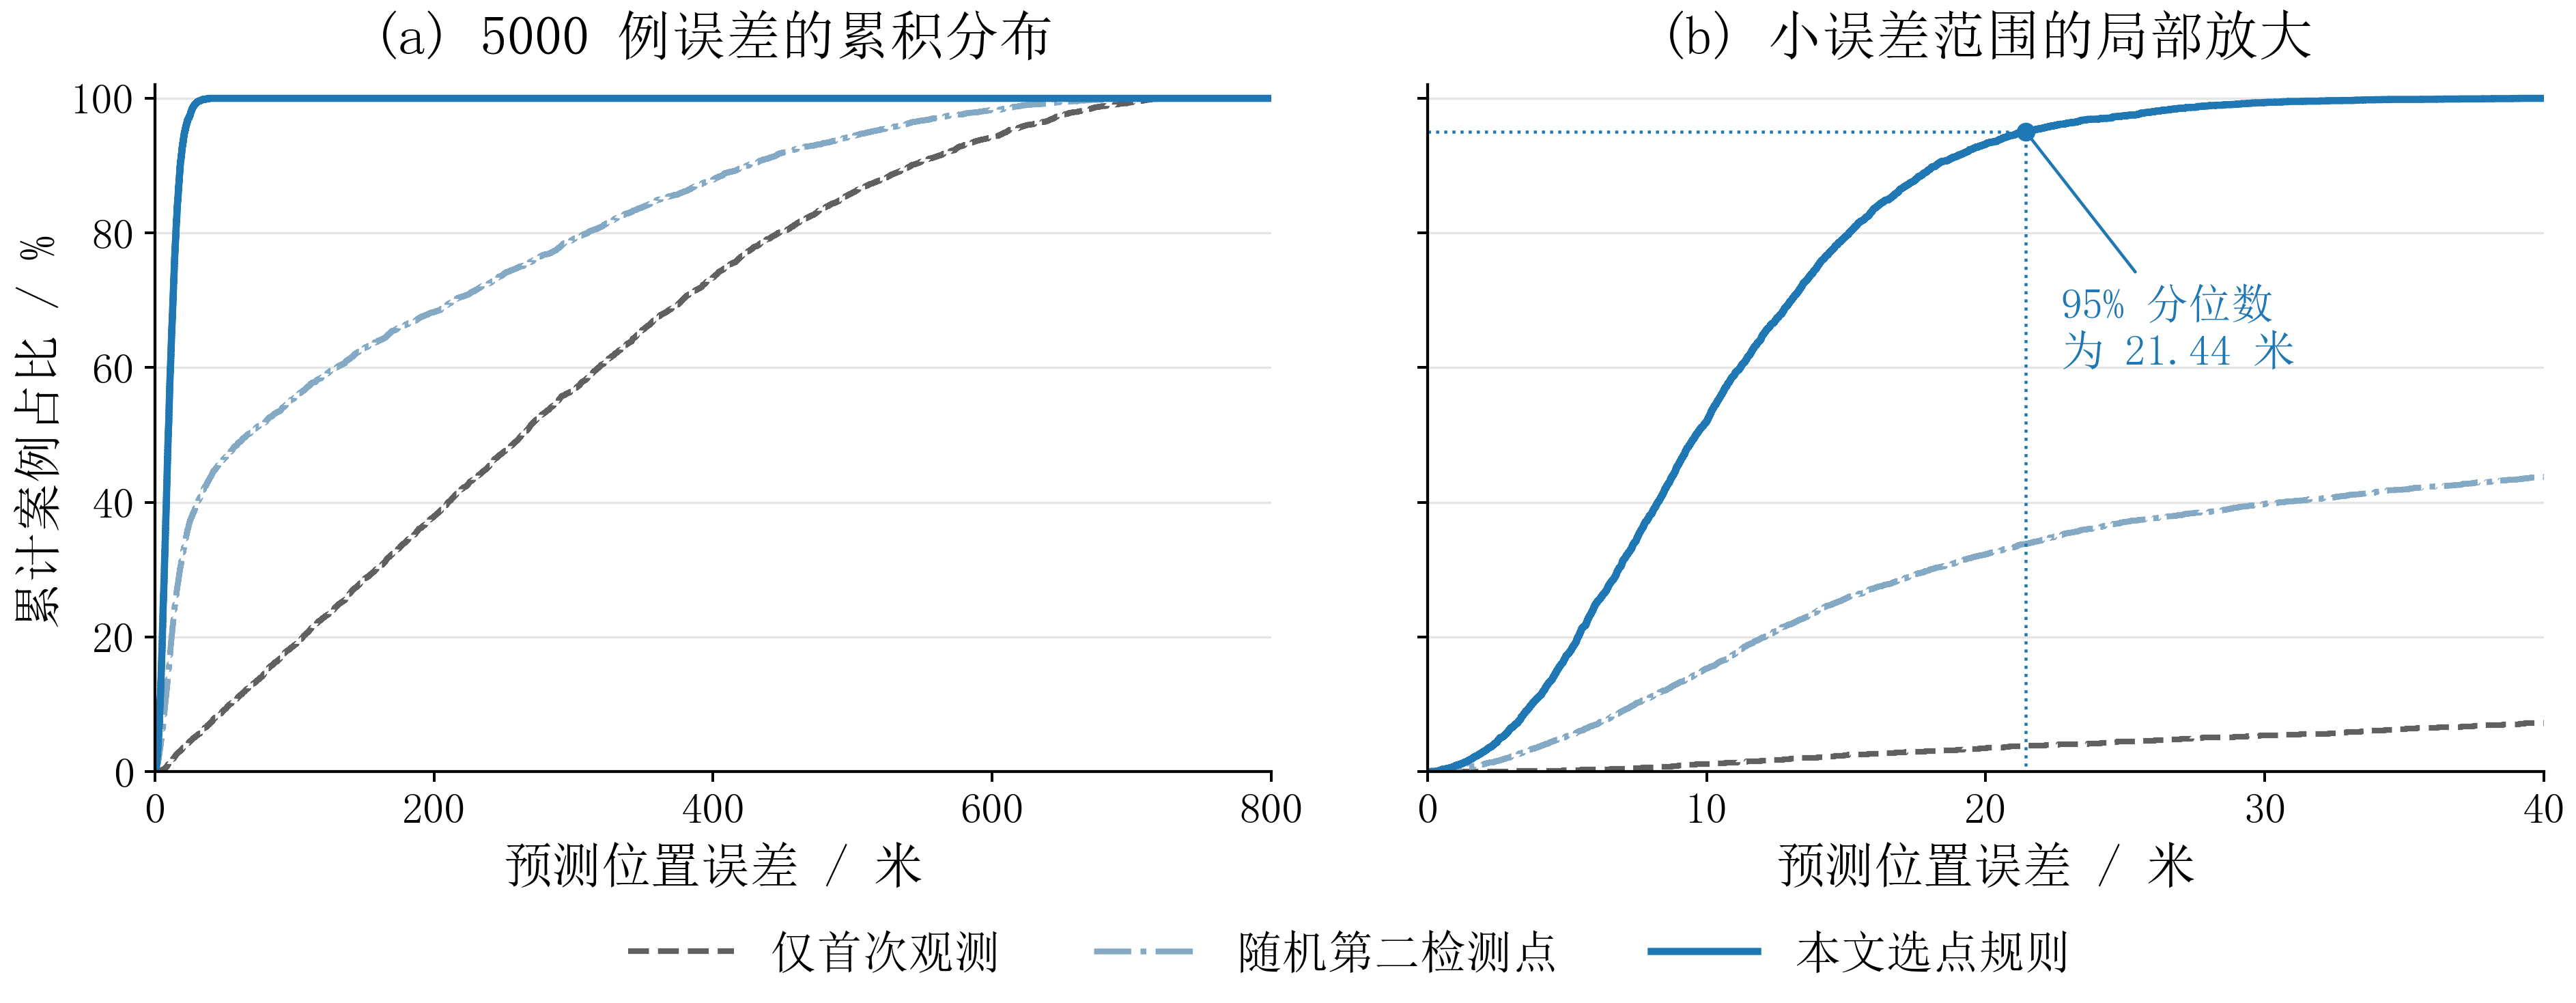
\includegraphics[width=\linewidth]{figures/q2_prediction_error_ecdf.png}
\caption{同批5000例中三种规则的预测误差累积分布}\label{fig:q2-error-ecdf}
\end{figure}

\FloatBarrier
\section{问题三的模型建立与求解}

无线电源搜索可根据观测条件调整不同阶段的行动策略\textsuperscript{\cite{ref4}}。前两问以单个干扰源为对象，根据示向度缩小位置范围，并比较不同检测位置的定位效果。第三问中，机器狗既要处理已经发现的源，又要继续排查尚未发现的源，两类任务共用同一条行进路线。一次新的观测不仅改变定位区域，也可能增加清除任务或减少后续巡测范围。因此，本问建立``基于覆盖约束的搜索-清除联合规划模型''，在维持排查完整性的前提下，设计机器狗的寻路策略。

\subsection{模型建立}

\subsubsection{状态与行动}

源搜索可通过观测更新信念状态并据此选择后续行动\textsuperscript{\cite{ref7}}。我们定义离散指标 \(t=0,1,\ldots\) 表示第 \(t\) 个行动开始前的决策步，该指标以行动序号计量。频道集合记为 \(\mathcal C=\{1,\ldots,20\}\)，目标可能出现的区域为：
\[
\Omega=\{g\in\mathbb R^2:\|g\|_2\le1800\}
\]

在决策步 \(t\)，记机器狗当前位置为 \(p_t\)，测向机当前频道为 \(\kappa_t\)。记 \(\mathcal D_t\) 为已发现但尚未清除的频道集合，\(\mathcal N_t\) 为尚未发现干扰源的频道集合。当频道被成功清除时，不再属于上述两个集合。

对 \(c\in\mathcal D_t\)，源位置 \(g\) 与该源在频道 \(c\) 的有效接收半径 \(R\) 构成一个组合 \((g,R)\)。能够同时解释该频道截至当前全部检测结果的组合构成集合 \(\mathcal X_{c,t}\)：
\[
\mathcal X_{c,t}\subseteq\Omega\times[1000,1500]
\]

其中，\(g\) 为源的可能位置，\(R\) 为该源在频道 \(c\) 的有效接收半径，同一个源在历次检测中对应同一个 \(R\)。\(F_{c,t}=\operatorname{proj}_g\mathcal X_{c,t}\) 为这些组合对应的定位区域，由每个组合中取出位置分量 \(g\) 得到。对 \(c\in\mathcal N_t\)，以 \(H^-_{c,t}\) 记录截至当前在频道 \(c\) 上测得无信号的全部检测点坐标，该频道尚未排除的目标区域为：
\[
U_{c,t}
=
\Omega\setminus
\bigcup_{h\in H^-_{c,t}}\overline B(h,1000)
\]

其中，\(h\) 为频道 \(c\) 的无信号检测点坐标，\(\overline B(h,1000)\) 为以 \(h\) 为圆心、半径 1000 米的闭圆盘。全向源的接收半径不小于 1000 米，由此在 \(h\) 处测得无信号即排除以 \(h\) 为圆心、半径 1000 米的圆盘。借鉴马尔可夫决策过程的序贯决策思想，定义信息状态为：
\[
S_t=
\left(
p_t,\kappa_t,\mathcal D_t,\mathcal N_t,
\{\mathcal X_{c,t}:c\in\mathcal D_t\},
\{H^-_{c,t},U_{c,t}:c\in\mathcal N_t\}
\right)
\tag{20}
\]

机器狗在状态 \(S_t\) 下选择行动：
\[
a_t=(o_t,q_t,c_t)=\pi(S_t)
\tag{21}
\]

其中，\(o_t\in\{\text{检测},\text{清除}\}\) 为本次行动类型，\(q_t\) 为本次行动的位置，\(c_t\) 为目标频道，\(\pi\) 为根据当前状态选择下一行动的策略。

\subsubsection{状态转移}

记 \(y_t\) 为行动 \(a_t\) 得到的反馈，下一状态为：
\[
S_{t+1}=\Phi(S_t,a_t,y_t),
\qquad
p_{t+1}=q_t,
\qquad
\kappa_{t+1}=
\begin{cases}
c_t,&o_t=\text{检测},\\
\kappa_t,&o_t=\text{清除}
\end{cases}
\tag{22}
\]

除下述与频道 \(c_t\) 有关的状态外，其余频道的信息保持不变。状态转移算子 \(\Phi\) 按行动类型分为检测与清除两部分。

\paragraph{检测行动}

检测反馈可能为近距离、示向度或无信号。根据频道此前是否已被发现，模型分别进行如下更新。

（1）检测已发现频道。 当 \(c_t\in\mathcal D_t\) 时，该频道此前得到的全部可能组合为 \(\mathcal X_{c_t,t}\)。三类反馈分别给出：
\[
\mathcal X_{c_t,t+1}=
\begin{cases}
\{(g,R)\in\mathcal X_{c_t,t}:\|g-q_t\|_2\le5\},
&y_t=\text{近距离},\\[1mm]
\{(g,R)\in\mathcal X_{c_t,t}:g\in W(q_t,\beta),\ 5<\|g-q_t\|_2\le R\},
&y_t=\text{示向度 }\beta,\\[1mm]
\{(g,R)\in\mathcal X_{c_t,t}:\|g-q_t\|_2>R\},
&y_t=\text{无信号}
\end{cases}
\tag{23a}
\]

更新后的定位区域为：
\[
F_{c_t,t+1}=\operatorname{proj}_g\mathcal X_{c_t,t+1}
\]

上述更新均在 \(\mathcal X_{c_t,t}\) 给出的组合中进行，因此更新后的组合仍能解释该频道此前的全部检测结果。

（2）检测未发现频道。 当 \(c_t\in\mathcal N_t\) 时，根据返回结果分为无信号与有信号两种情况。

\begin{enumerate}
\def\labelenumi{\arabic{enumi}.}
\tightlist
\item
  返回无信号。 该频道仍未被发现。由于全向源的接收半径不小于1000米，可排除检测点周围1000米范围：
\end{enumerate}
\[
H^-_{c_t,t+1}=H^-_{c_t,t}\cup\{q_t\},
   \qquad
   U_{c_t,t+1}=U_{c_t,t}\setminus\overline B(q_t,1000)
   \tag{23b}
\]

\begin{enumerate}
\def\labelenumi{\arabic{enumi}.}
\setcounter{enumi}{1}
\tightlist
\item
  返回信号。 该频道被发现。先根据此前的全部无信号记录构造：
\end{enumerate}
\[
\mathcal X^-_{c_t,t}
   =
   \{(g,R)\in\Omega\times[1000,1500]:
   \|g-h\|_2>R,\ \forall h\in H^-_{c_t,t}\}
\]

再根据本次信号类型更新：
\[
\mathcal X_{c_t,t+1}=
   \begin{cases}
   \{(g,R)\in\mathcal X^-_{c_t,t}:\|g-q_t\|_2\le5\},
   &y_t=\text{近距离},\\[1mm]
   \{(g,R)\in\mathcal X^-_{c_t,t}:g\in W(q_t,\beta),\ 5<\|g-q_t\|_2\le R\},
   &y_t=\text{示向度 }\beta
   \end{cases}
   \tag{23c}
\]

随后更新定位区域与频道集合为：
\[
F_{c_t,t+1}=\operatorname{proj}_g\mathcal X_{c_t,t+1},
   \qquad
   \mathcal D_{t+1}=\mathcal D_t\cup\{c_t\},
   \qquad
   \mathcal N_{t+1}=\mathcal N_t\setminus\{c_t\}
\]

\paragraph{清除行动}

清除行动仅针对 \(c_t\in\mathcal D_t\) 执行，并根据结果分为以下两种情况。

\begin{enumerate}
\def\labelenumi{\arabic{enumi}.}
\tightlist
\item
  清除成功。 该频道的干扰源已被处理，将其从待清除集合中删除：
\end{enumerate}
\[
\mathcal D_{t+1}=\mathcal D_t\setminus\{c_t\}
\]

\begin{enumerate}
\def\labelenumi{\arabic{enumi}.}
\setcounter{enumi}{1}
\tightlist
\item
  清除失败。 由失败反馈可知真实位置不在清除点周围20米内，因此更新：
\end{enumerate}
\[
\mathcal X_{c_t,t+1}
   =
   \{(g,R)\in\mathcal X_{c_t,t}:\|g-q_t\|_2>20\},
   \qquad
   F_{c_t,t+1}=\operatorname{proj}_g\mathcal X_{c_t,t+1}
   \tag{23d}
\]

\subsubsection{保证清除区域与候选行动}

对 \(c\in\mathcal D_t\)，定义保证清除区域：
\[
\mathcal G_{c,t}
=
\left\{q\in\mathbb R^2:
\sup_{g\in F_{c,t}}\|g-q\|_2\le20
\right\}
=
\bigcap_{g\in F_{c,t}}\overline B(g,20)
\tag{24}
\]

\(\mathcal G_{c,t}\) 中的任一点到全部可能真实位置的距离均不超过20米，因而能够保证清除成功。由最小包围圆的定义得：
\[
\mathcal G_{c,t}\ne\varnothing
\quad\Longleftrightarrow\quad
\rho(F_{c,t})\le20
\]

当 \(\mathcal G_{c,t}\ne\varnothing\) 时，选择距离当前位置最近的保证清除点：
\[
q_{c,t}^{\mathrm{clr}}
\in
\arg\min_{q\in\mathcal G_{c,t}}\|q-p_t\|_2,
\]

并构造清除候选行动集合：
\[
\mathcal A_t^{\mathrm{clr}}
=
\left\{
(\text{清除},q_{c,t}^{\mathrm{clr}},c):
c\in\mathcal D_t,
\mathcal G_{c,t}\ne\varnothing
\right\}
\tag{25}
\]

当 \(\mathcal G_{c,t}=\varnothing\) 时，当前信息不足以保证清除成功，故后续检测用于缩小 \(F_{c,t}\)。因此，\(\mathcal G_{c,t}\) 决定频道 \(c\) 在当前阶段生成``补充检测行动''还是``保证清除行动''，而 \(\mathcal A_t^{\mathrm{clr}}\) 将几何定位结果直接转化为后续路线中的可执行任务。

\subsubsection{完整排查与终止条件}

对每个 \(c\in\mathcal N_t\)，记 \(\mathcal P_{c,t}\) 为后续计划检测该频道的位置集合。由于未知干扰源的接收半径至少为1000米，为完整排查当前未排除区域，要求：
\[
U_{c,t}
\subseteq
\bigcup_{q\in\mathcal P_{c,t}}\overline B(q,1000),
\qquad c\in\mathcal N_t
\tag{26}
\]

当所有已发现源均已清除，且所有尚未发现频道的可能区域均已排空时，任务完成。策略 \(\pi\) 的终止步定义为：
\[
\tau_\pi
=
\inf\left\{
t:\mathcal D_t=\varnothing,
\quad
U_{c,t}=\varnothing,\ \forall c\in\mathcal N_t
\right\}
\tag{27}
\]

模型将``退出''并入终止条件，任务在满足式（27）时自然终止。由于每次行动均满足 \(p_{t+1}=q_t\)，因此，最终位置也将满足 \(p_{\tau_\pi}=q_{\tau_\pi-1}\)。

\subsubsection{时间代价与优化目标}

行动 \(a_t\) 的实际耗时为：
\[
\ell(S_t,a_t,y_t)
=
\frac{\|q_t-p_t\|_2}{5}
+
\begin{cases}
5+\mathbf 1_{\{c_t\ne\kappa_t\}},&o_t=\text{检测},\\[1mm]
5,&o_t=\text{清除且成功},\\[1mm]
3,&o_t=\text{清除且失败}
\end{cases}
\tag{28}
\]

其中，检测完成后测向机频道变为 \(c_t\)，清除操作不改变当前频道。策略 \(\pi\) 的完整任务时间为：
\[
T_{\mathrm{exit}}(\pi)
=
\sum_{t=0}^{\tau_\pi-1}\ell(S_t,a_t,y_t)
\tag{29}
\]

问题三的优化目标为：
\[
\min_{\pi\in\Pi_{\mathrm{adm}}}
\mathbb E\!\left[T_{\mathrm{exit}}(\pi)\right],
\tag{30}
\]

其中，\(\Pi_{\mathrm{adm}}\) 为满足状态转移式（22）---（23）、完整排查约束式（26）与终止条件式（27）的可行策略集合。式（27）保证全部干扰源最终被发现并清除，式（30）则在此前提下比较不同策略的平均完成时间。

\subsection{模型的滚动规划求解}

\subsubsection{模型特点与算法选择}

采用精确动态规划时，价值函数满足：
\[
V(S)
=
\min_{a\in\mathcal A(S)}
\mathbb E\!\left[
\ell(S,a,Y)+V\bigl(\Phi(S,a,Y)\bigr)
\mid S,a
\right],
\tag{31}
\]

其中，\(\mathcal A(S)\) 为当前状态下的可行行动集合。然而因为直接求解式（31）的计算量过大，所以我们借鉴模型预测控制的滚动优化思想，采用``基于条件场景评估的启发式滚动规划算法''：由式（26）保证排查的完整性，利用问题二的定位区域更新与选点方法处理已发现源，再通过有限候选路线与条件场景比较当前行动。每次只执行所选路线中的第一个行动，并根据反馈重新计算下一步。

\subsubsection{当前候选行动与条件场景}

在状态 \(S_t\) 下构造三类候选行动：

\begin{enumerate}
\def\labelenumi{\arabic{enumi}.}
\tightlist
\item
  对 \(c\in\mathcal N_t\)，根据式（26）生成未知频道检测行动，组成 \(\mathcal A_t^{\mathrm{scan}}\)；
\item
  对 \(c\in\mathcal D_t\) 且 \(\mathcal G_{c,t}=\varnothing\)，根据当前 \(F_{c,t}\) 与问题二的选点方法生成补充检测行动，组成 \(\mathcal A_t^{\mathrm{loc}}\)；
\item
  对 \(c\in\mathcal D_t\) 且 \(\mathcal G_{c,t}\ne\varnothing\)，按式（25）生成保证清除行动，组成 \(\mathcal A_t^{\mathrm{clr}}\)。
\end{enumerate}

由此得到：
\[
\mathcal A_t
=
\mathcal A_t^{\mathrm{scan}}
\cup\mathcal A_t^{\mathrm{loc}}
\cup\mathcal A_t^{\mathrm{clr}}
\]

仅比较当前已经生成的行动会忽略后续可能发现的新源。为估计这部分附加代价，我们根据未知频道的无信号历史构造条件场景。条件于频道 \(c\) 确实存在干扰源，候选位置 \(g\) 处允许的接收半径上界与相容权重为：
\[
R^{\max}_{c,t}(g)
=
\min\left\{
1500,
\min_{h\in H^-_{c,t}}\|g-h\|_2
\right\},
\qquad
w_{c,t}(g)
=
\left[R^{\max}_{c,t}(g)-1000\right]_+
\tag{32}
\]

当 \(H^-_{c,t}=\varnothing\) 时取 \(R^{\max}_{c,t}(g)=1500\)。按归一化后的 \(w_{c,t}(g)\) 抽取潜在位置，并结合10---16个源、频道互不重复的条件生成 \(B\) 个场景。

\subsubsection{候选路线评价}

由当前候选行动，我们构造若干从 \(p_t\) 出发的开放路线，记其集合为 \(\Sigma_t\)。对 \(\sigma\in\Sigma_t\)，记完成当前确定行动的代价为 \(C_t^{\mathrm{known}}(\sigma)\)；在场景 \(\omega\) 下，将可能新发现的源插入其首次可检测位置之后，产生的附加移动距离记为 \(\Delta L_t(\sigma,\omega)\)。

设频道 \(c\) 当前剩余的检测行动数为 \(k_{c,t}\)，场景 \(\omega\) 中实际存在源的未发现频道集合为 \(E(\omega)\)，频道 \(c\) 首次被发现前执行的检测行动数为 \(j_c(\sigma,\omega)\)，则未来频道检测次数近似为：
\[
N_t^{\mathrm{future}}(\sigma,\omega)
=
\sum_{c\in\mathcal N_t\setminus E(\omega)}k_{c,t}
+
\sum_{c\in E(\omega)}j_c(\sigma,\omega)
\]

候选路线的代理代价取为：
\[
\widetilde T_t(\sigma,\omega)
=
C_t^{\mathrm{known}}(\sigma)
+\frac{\Delta L_t(\sigma,\omega)}{5}
+6N_t^{\mathrm{future}}(\sigma,\omega)
\tag{33}
\]

其中，6秒近似一次检测与一次频道切换的代价，并选择：
\[
\sigma_t^*
\in
\arg\min_{\sigma\in\Sigma_t}
\frac1B\sum_{b=1}^{B}\widetilde T_t(\sigma,\omega_b)
\tag{34}
\]

滚动策略取所选路线的第一个行动，即：
\[
\pi_{\mathrm{roll}}(S_t)=\operatorname{First}(\sigma_t^*)
\]

图\ref{fig:q3-scenario-routes}以同一条件场景说明式（33）的代价估计。图中\(g\)为场景中假设存在的频道\(c\)干扰源，\(q_1,q_2\)为巡测点，\(A,B\)分别为补测与清除任务的执行位置。

\begin{figure}[H]
\centering
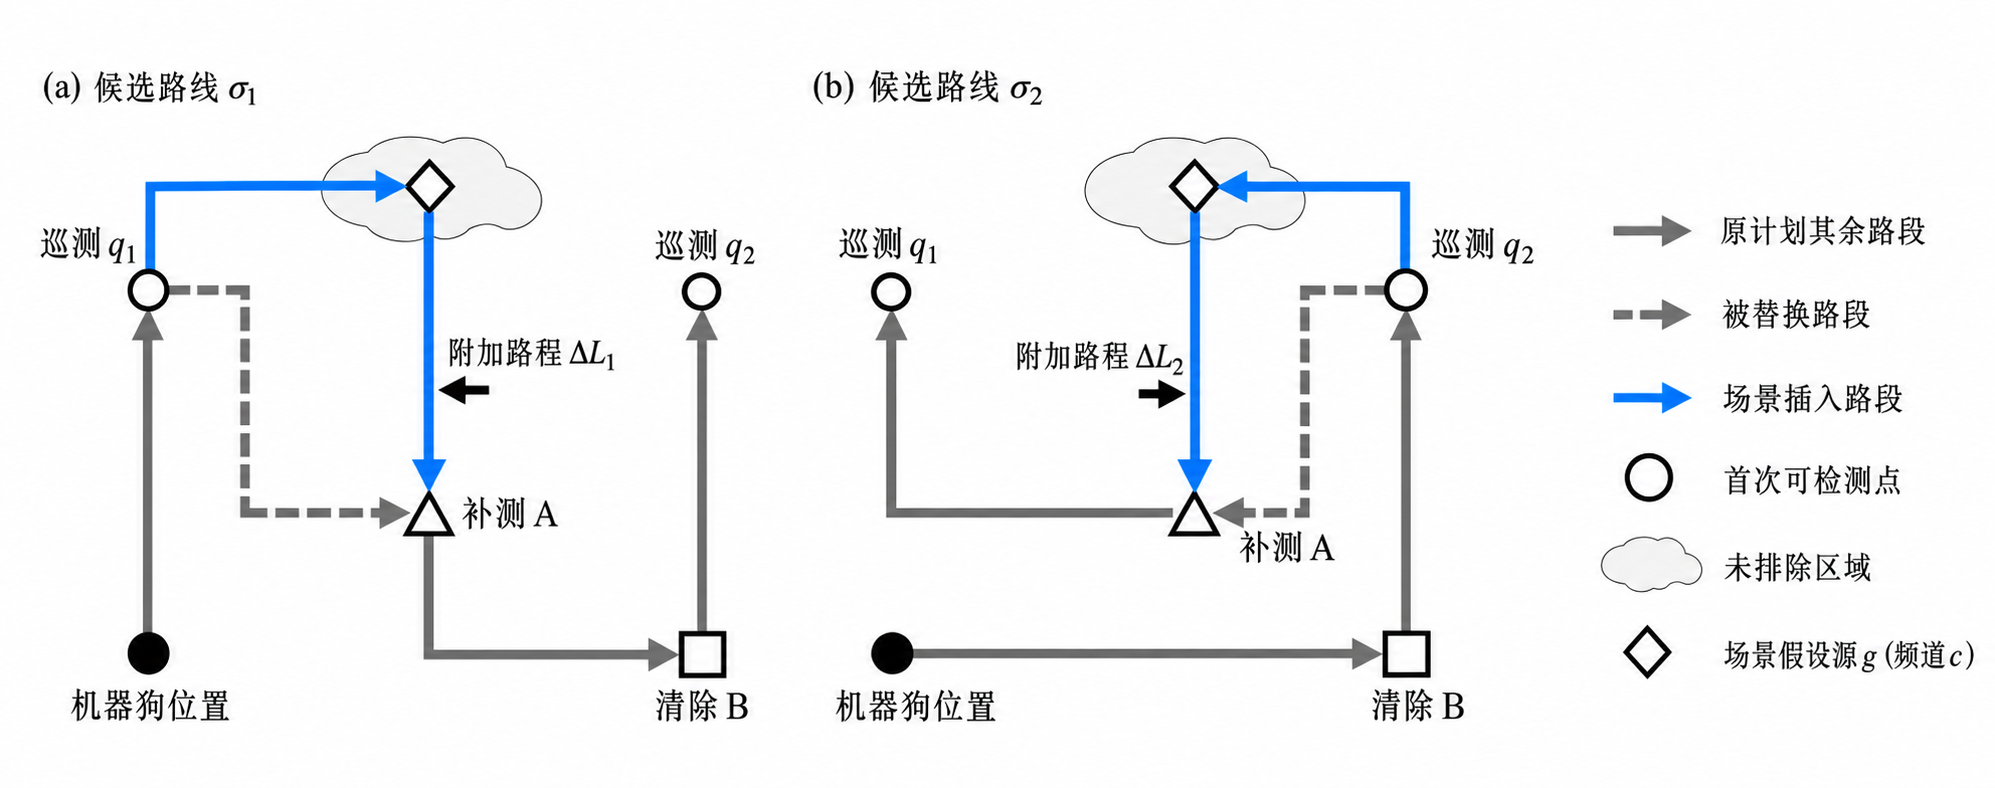
\includegraphics[width=\linewidth]{figures/q3_conditional_route_evaluation_paper.png}
\caption{条件场景下候选路线的附加代价估计}\label{fig:q3-scenario-routes}
\end{figure}

两条路线分别先在\(q_1\)、\(q_2\)检测到该假设源，因此在代价估计中用蓝色路段\(q_i\to g\to A\)替换灰色虚线路段\(q_i\to A\)。图中\(\Delta L_i\)为两段蓝线路程之和减去被替换路段的长度。发现频道\(c\)后，后续巡测点跳过该频道；将这一检测次数变化与附加移动计入式（33），再按式（34）对同批场景取平均，即得到候选路线的比较依据。

\subsubsection{滚动求解步骤}

\textbf{Step 1　初始化状态。} 令 \(p_0=(0,0)\)、\(\kappa_0=1\)、\(\mathcal D_0=\varnothing\)、\(\mathcal N_0=\mathcal C\)，并对所有频道取 \(H^-_{c,0}=\varnothing\)、\(U_{c,0}=\Omega\)。

\textbf{Step 2　生成未知频道检测行动。} 根据各频道当前的 \(U_{c,t}\) 生成满足式（26）的检测位置，并明确每个位置对应的检测频道，得到 \(\mathcal A_t^{\mathrm{scan}}\)。计算时采用可细分方格保守表示 \(U_{c,t}\)，仅当方格被排除圆完整覆盖时才删除，使有限采样点的覆盖判定对应连续区域的排除。

\textbf{Step 3　生成补充检测与清除行动。} 对每个 \(c\in\mathcal D_t\)，当 \(\mathcal G_{c,t}=\varnothing\) 时，根据当前定位区域生成补充检测行动；当 \(\mathcal G_{c,t}\ne\varnothing\) 时，按式（25）生成保证清除行动。二者分别组成 \(\mathcal A_t^{\mathrm{loc}}\) 与 \(\mathcal A_t^{\mathrm{clr}}\)。

\textbf{Step 4　构造候选路线。} 将三类候选行动组成 \(\mathcal A_t\)，从当前位置出发生成若干开放路线，并利用多起点、任务重插入与两交换（2-opt）调整行动次序；所有调整均保持式（26）的完整覆盖要求。

\textbf{Step 5　评价并选择路线。} 根据式（32）抽取同一批条件场景，按式（33）计算各候选路线的平均代理代价，并由式（34）选出当前路线。

\textbf{Step 6　执行首个行动并更新状态。} 仅执行 \(\sigma_t^*\) 的第一个行动，根据真实反馈按式（22）---（23）完成状态转移，再重新生成候选行动与路线。

\textbf{Step 7　检查终止条件。} 当式（27）成立时，任务结束，并按式（29）记录完整任务时间；否则返回 Step 2 继续滚动求解。

\subsection{独立案例验证}

在开发案例上确定策略及参数后，我们使用另外1000个随机案例检验本文策略。全部案例均完成清除并正常退出，剩余源总数为0。本文算法的平均每源耗时为212.77秒/源。

图\ref{fig:old4}给出逐例按源数归一化后的耗时分布与构成。95\%的案例每源完整退出耗时不超过269.92秒；失败清除的平均每源耗时仅为0.39秒。本文策略在1000个独立案例中实现了100\%的全清与正常退出率，失败清除的直接耗时占比仅为0.18\%，展现了可靠的任务完成能力与极低的无效清除直接开销。

\begin{figure}[H]
\centering
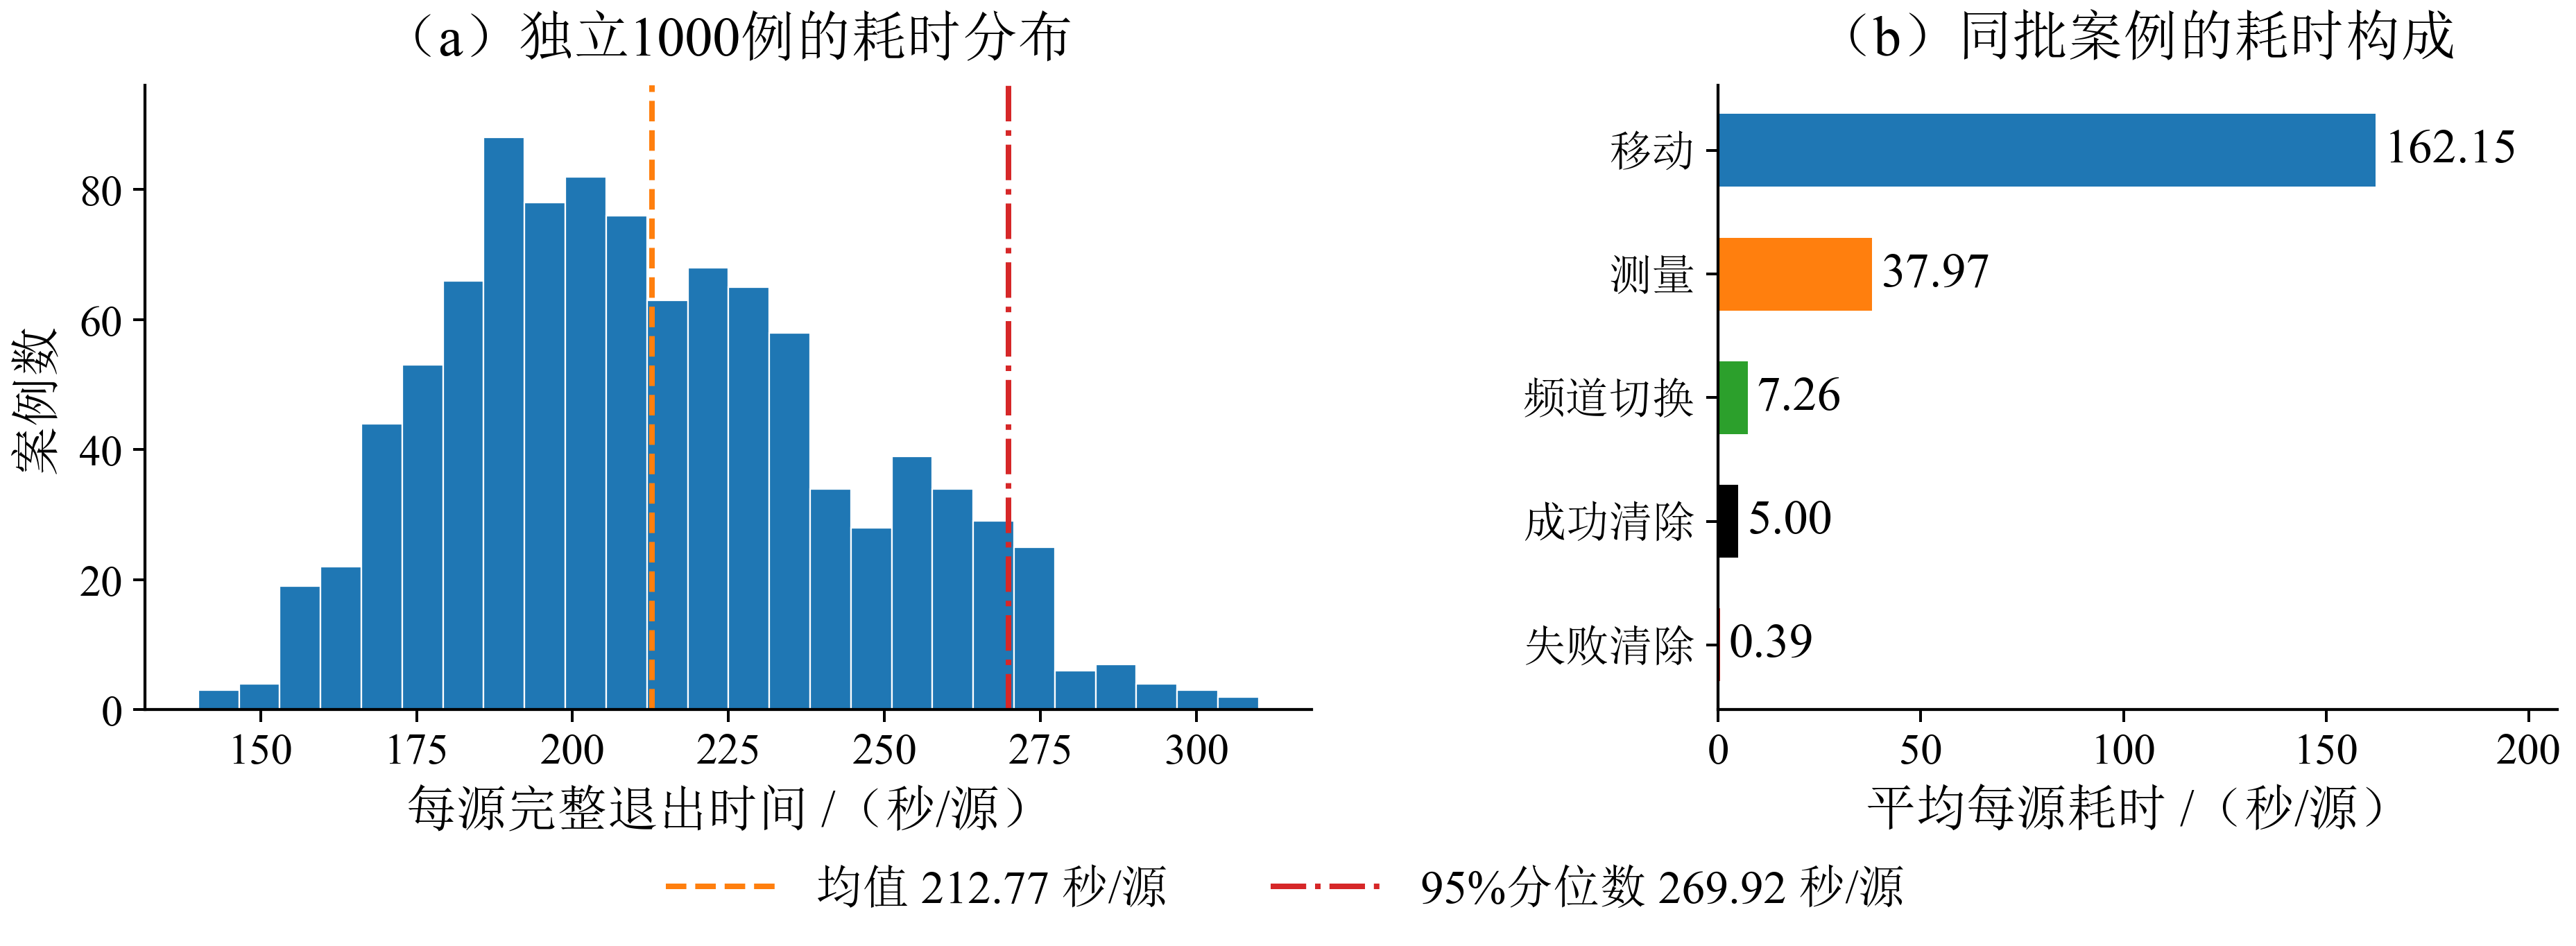
\includegraphics[width=0.96\linewidth,height=0.68\textheight,keepaspectratio]{figures/q3_time_distribution.png}
\caption{独立案例的每源耗时分布与耗时构成}\label{fig:old4}
\end{figure}

\subsection{正式测试结果}

我们在模拟器中完成第三问的三次正式测试，均清除了全部干扰源，结果见表\ref{tab:old7}。平均定位清除时间为该例完整退出虚拟耗时与清除源数的比值，程序运行时间为模拟器记录的现实执行时长。

\begingroup
\small
\setlength{\tabcolsep}{4pt}
\setlength{\TableInnerWidth}{\dimexpr\linewidth-6\tabcolsep\relax}
\renewcommand{\arraystretch}{1.22}
\begin{longtable}{@{}>{\centering\arraybackslash}p{0.390\TableInnerWidth}>{\centering\arraybackslash}p{0.170\TableInnerWidth}>{\centering\arraybackslash}p{0.260\TableInnerWidth}>{\centering\arraybackslash}p{0.180\TableInnerWidth}@{}}
\caption{问题3正式测试结果}\label{tab:old7}\\
\toprule
测试案例编码 & 清除干扰源个数 & 平均定位清除时间 /（秒/源） & 程序运行时间 / 秒 \\
\midrule
\endfirsthead
\multicolumn{4}{c}{表\thetable\quad 问题3正式测试结果（续）}\\
\toprule
测试案例编码 & 清除干扰源个数 & 平均定位清除时间 /（秒/源） & 程序运行时间 / 秒 \\
\midrule
\endhead
\midrule
\multicolumn{4}{r}{续下页}\\
\endfoot
\bottomrule
\endlastfoot
UJBC-A4W9-A6FZ-XYQF & 15 & 175.896 & 1.999 \\
CQFE-KMZK-43Z9-VC6H & 12 & 217.896 & 1.478 \\
5P3S-DMUG-M4NP-N8W4 & 10 & 247.627 & 1.771 \\
\end{longtable}
\endgroup

\Needspace{0.50\textheight}
\subsection{灵敏度分析与消融实验}

由100例开发集选定消融项后，我们在另100例上配对验证。各组均全清并正常退出，剩余源与失败案例均为0。消融时仅在仍有巡测站时优先巡测，其余规则不变。

\begingroup
\renewcommand{\baselinestretch}{1.05}\fontsize{10.5}{13}\selectfont
\setlength{\tabcolsep}{3.5pt}
\setlength{\TableInnerWidth}{\dimexpr\linewidth-6\tabcolsep\relax}
\setlength{\LTpre}{3pt}\setlength{\LTpost}{3pt}
\renewcommand{\arraystretch}{1.05}
\begin{longtable}{@{}>{\centering\arraybackslash}p{0.32\TableInnerWidth}>{\centering\arraybackslash}p{0.23\TableInnerWidth}>{\centering\arraybackslash}p{0.25\TableInnerWidth}>{\centering\arraybackslash}p{0.20\TableInnerWidth}@{}}
\caption{灵敏度与消融的100例配对验证结果}\label{tab:q3-analysis}\\
\toprule
设置 & 平均完整耗时 / 秒 & 平均每源耗时 /（秒/源） & 失败清除次数 \\
\midrule
\endfirsthead
\multicolumn{4}{c}{表\thetable\quad 灵敏度与消融的100例配对验证结果（续）}\\
\toprule
设置 & 平均完整耗时 / 秒 & 平均每源耗时 /（秒/源） & 失败清除次数 \\
\midrule
\endhead
\midrule
\multicolumn{4}{r}{续下页}\\
\endfoot
\bottomrule
\endlastfoot
完整算法（\(B=64\)） & 2756.47 & 215.96 & 162 \\
\(B=16\) & 2757.10 & 215.95 & 159 \\
\(B=32\) & 2758.49 & 216.00 & 165 \\
巡测优先（\(B=64\)） & 3736.31 & 292.66 & 132 \\
\end{longtable}
\endgroup

\begin{figure}[H]
\centering
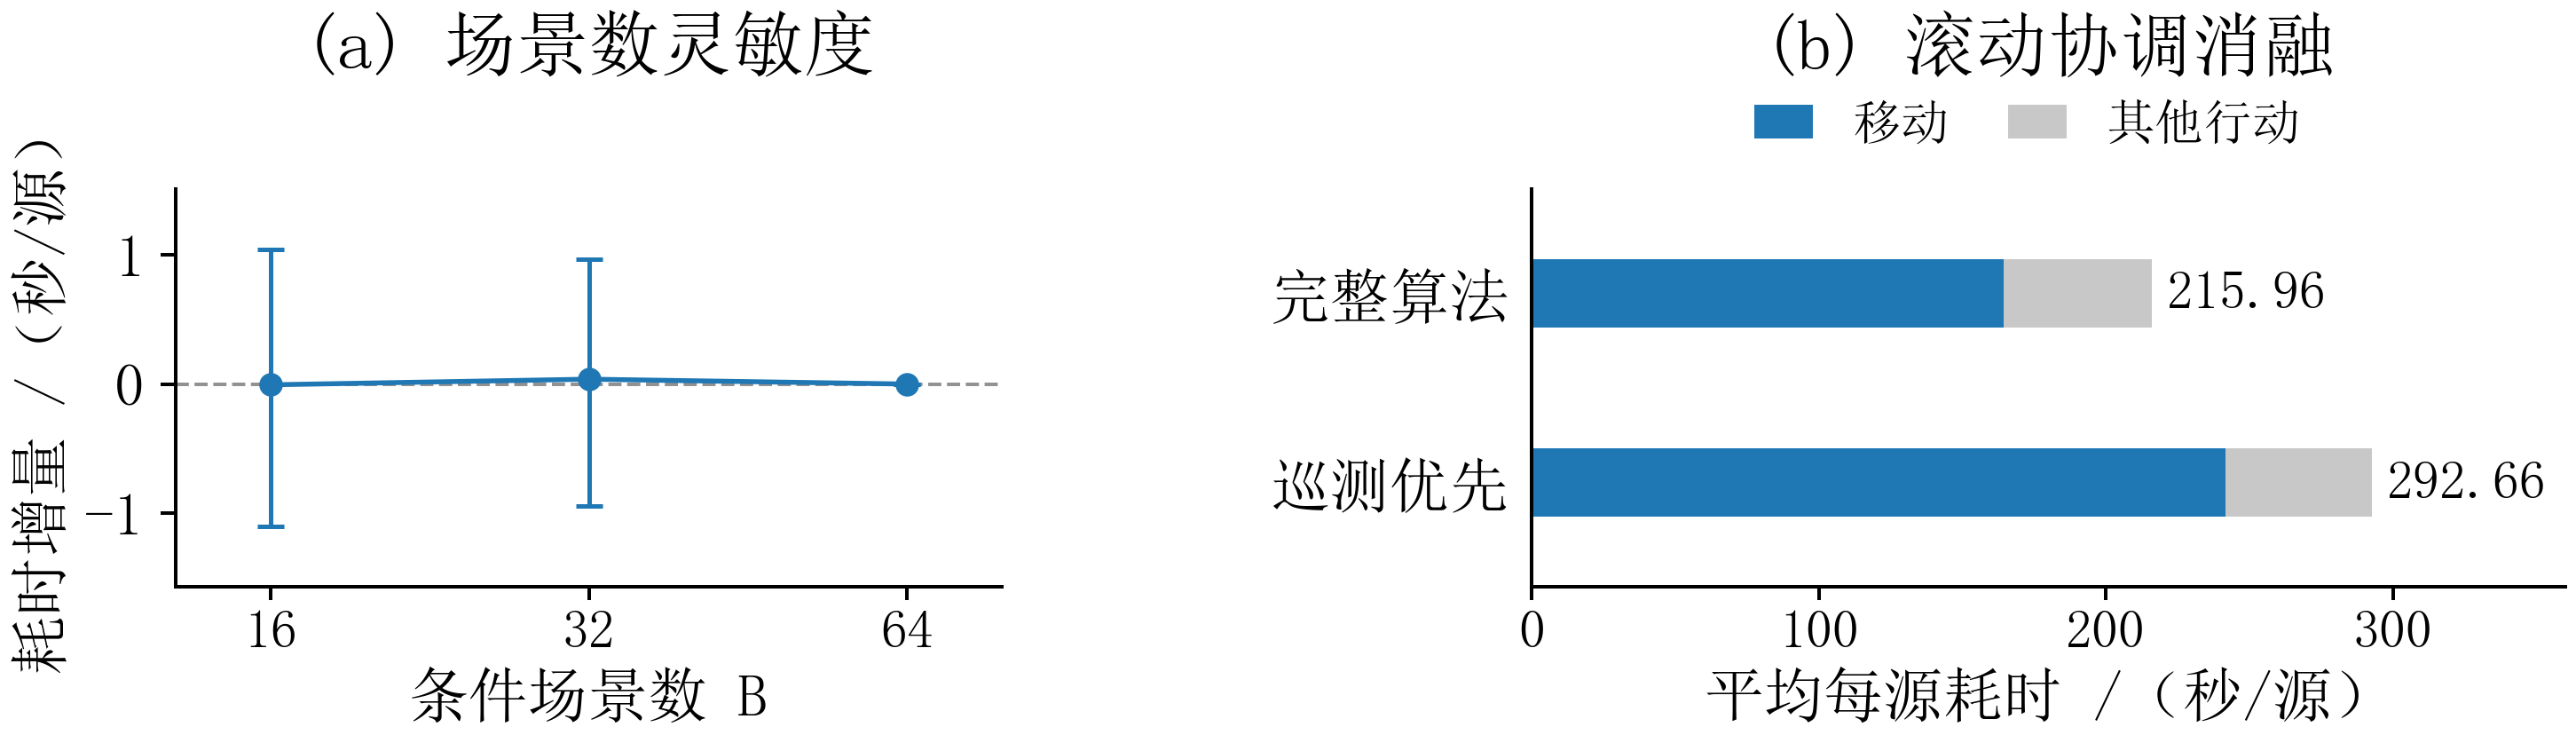
\includegraphics[width=\linewidth]{figures/q3_ablation_paired.png}
\caption{场景数灵敏度与滚动协调消融；左图以\(B=64\)为基准，误差棒为95\%配对区间}\label{fig:q3-analysis}
\end{figure}

灵敏度分析表明，算法的平均每源耗时在所测场景数范围内保持稳定，对该参数变化不敏感。消融实验表明，滚动协调通过减少移动开销，使平均每源耗时较巡测优先降低26.21\%。因此，在保证全部清除的前提下，穿插安排巡测与清除能够提高任务效率。

\FloatBarrier
\section{问题四的模型建立与求解}

第四问中，定向源即使距检测点不足1000米，也会因检测点处于发射背面而返回无信号，第三问的单点圆盘排除方法因而失效。我们据此建立``方向覆盖约束下的搜索-清除联合规划模型''，利用多点检测消除方向歧义，将距离与方向联合排查条件纳入第三问的滚动协同框架，安排搜索、定位与清除任务。

\subsection{模型建立}

\subsubsection{定向接收条件}

沿用第三问的状态与行动定义，由于第四问引入了定向干扰源，故我们将单源参数扩展为 \(x=(g,R,\phi,\zeta)\)，其中，\(\phi\) 为发射朝向，\(\zeta=0,1\) 分别表示全向源和定向源。令 \(\boldsymbol d(\phi)=(\cos\phi,\sin\phi)^{\mathsf T}\)，未清除源在检测点 \(s\) 处的接收条件为：
\[
\nu(s;x)=
\begin{cases}
\mathbf 1_{\{\|s-g\|_2\le R\}},&\zeta=0,\\
\mathbf 1_{\{\|s-g\|_2\le R\}}\mathbf 1_{\{\boldsymbol d(\phi)^{\mathsf T}(s-g)\ge0\}},&\zeta=1
\end{cases}
\tag{35}
\]

其中，\(\nu=1\) 表示能够接收信号，内积非负表示检测点位于180°发射半平面内。用式（35）替换第三问反馈更新中的接收条件：有信号时保留 \(\nu=1\) 的参数组合，并加入原有的距离或示向度约束；无信号时保留 \(\nu=0\) 的组合。同一源的位置、半径、朝向和类型保持固定，更新后的组合须满足历次反馈。

清除不受发射朝向限制，第三问的清除反馈更新及式（24）的保证清除区域继续适用。因此，本问新增的约束集中在未知频道的排查过程。

\subsubsection{完整排查与优化目标}

覆盖布局需考虑目标朝向对可观测性的影响\textsuperscript{\cite{ref6}}。单侧检测点可以同时处于发射背面；若检测点从不同方向包围潜在源位置，则至少有一点位于发射正面，如图\ref{fig:old5}所示。结合最小接收半径，这一关系可用于排除区域。

\begin{figure}[H]
\centering
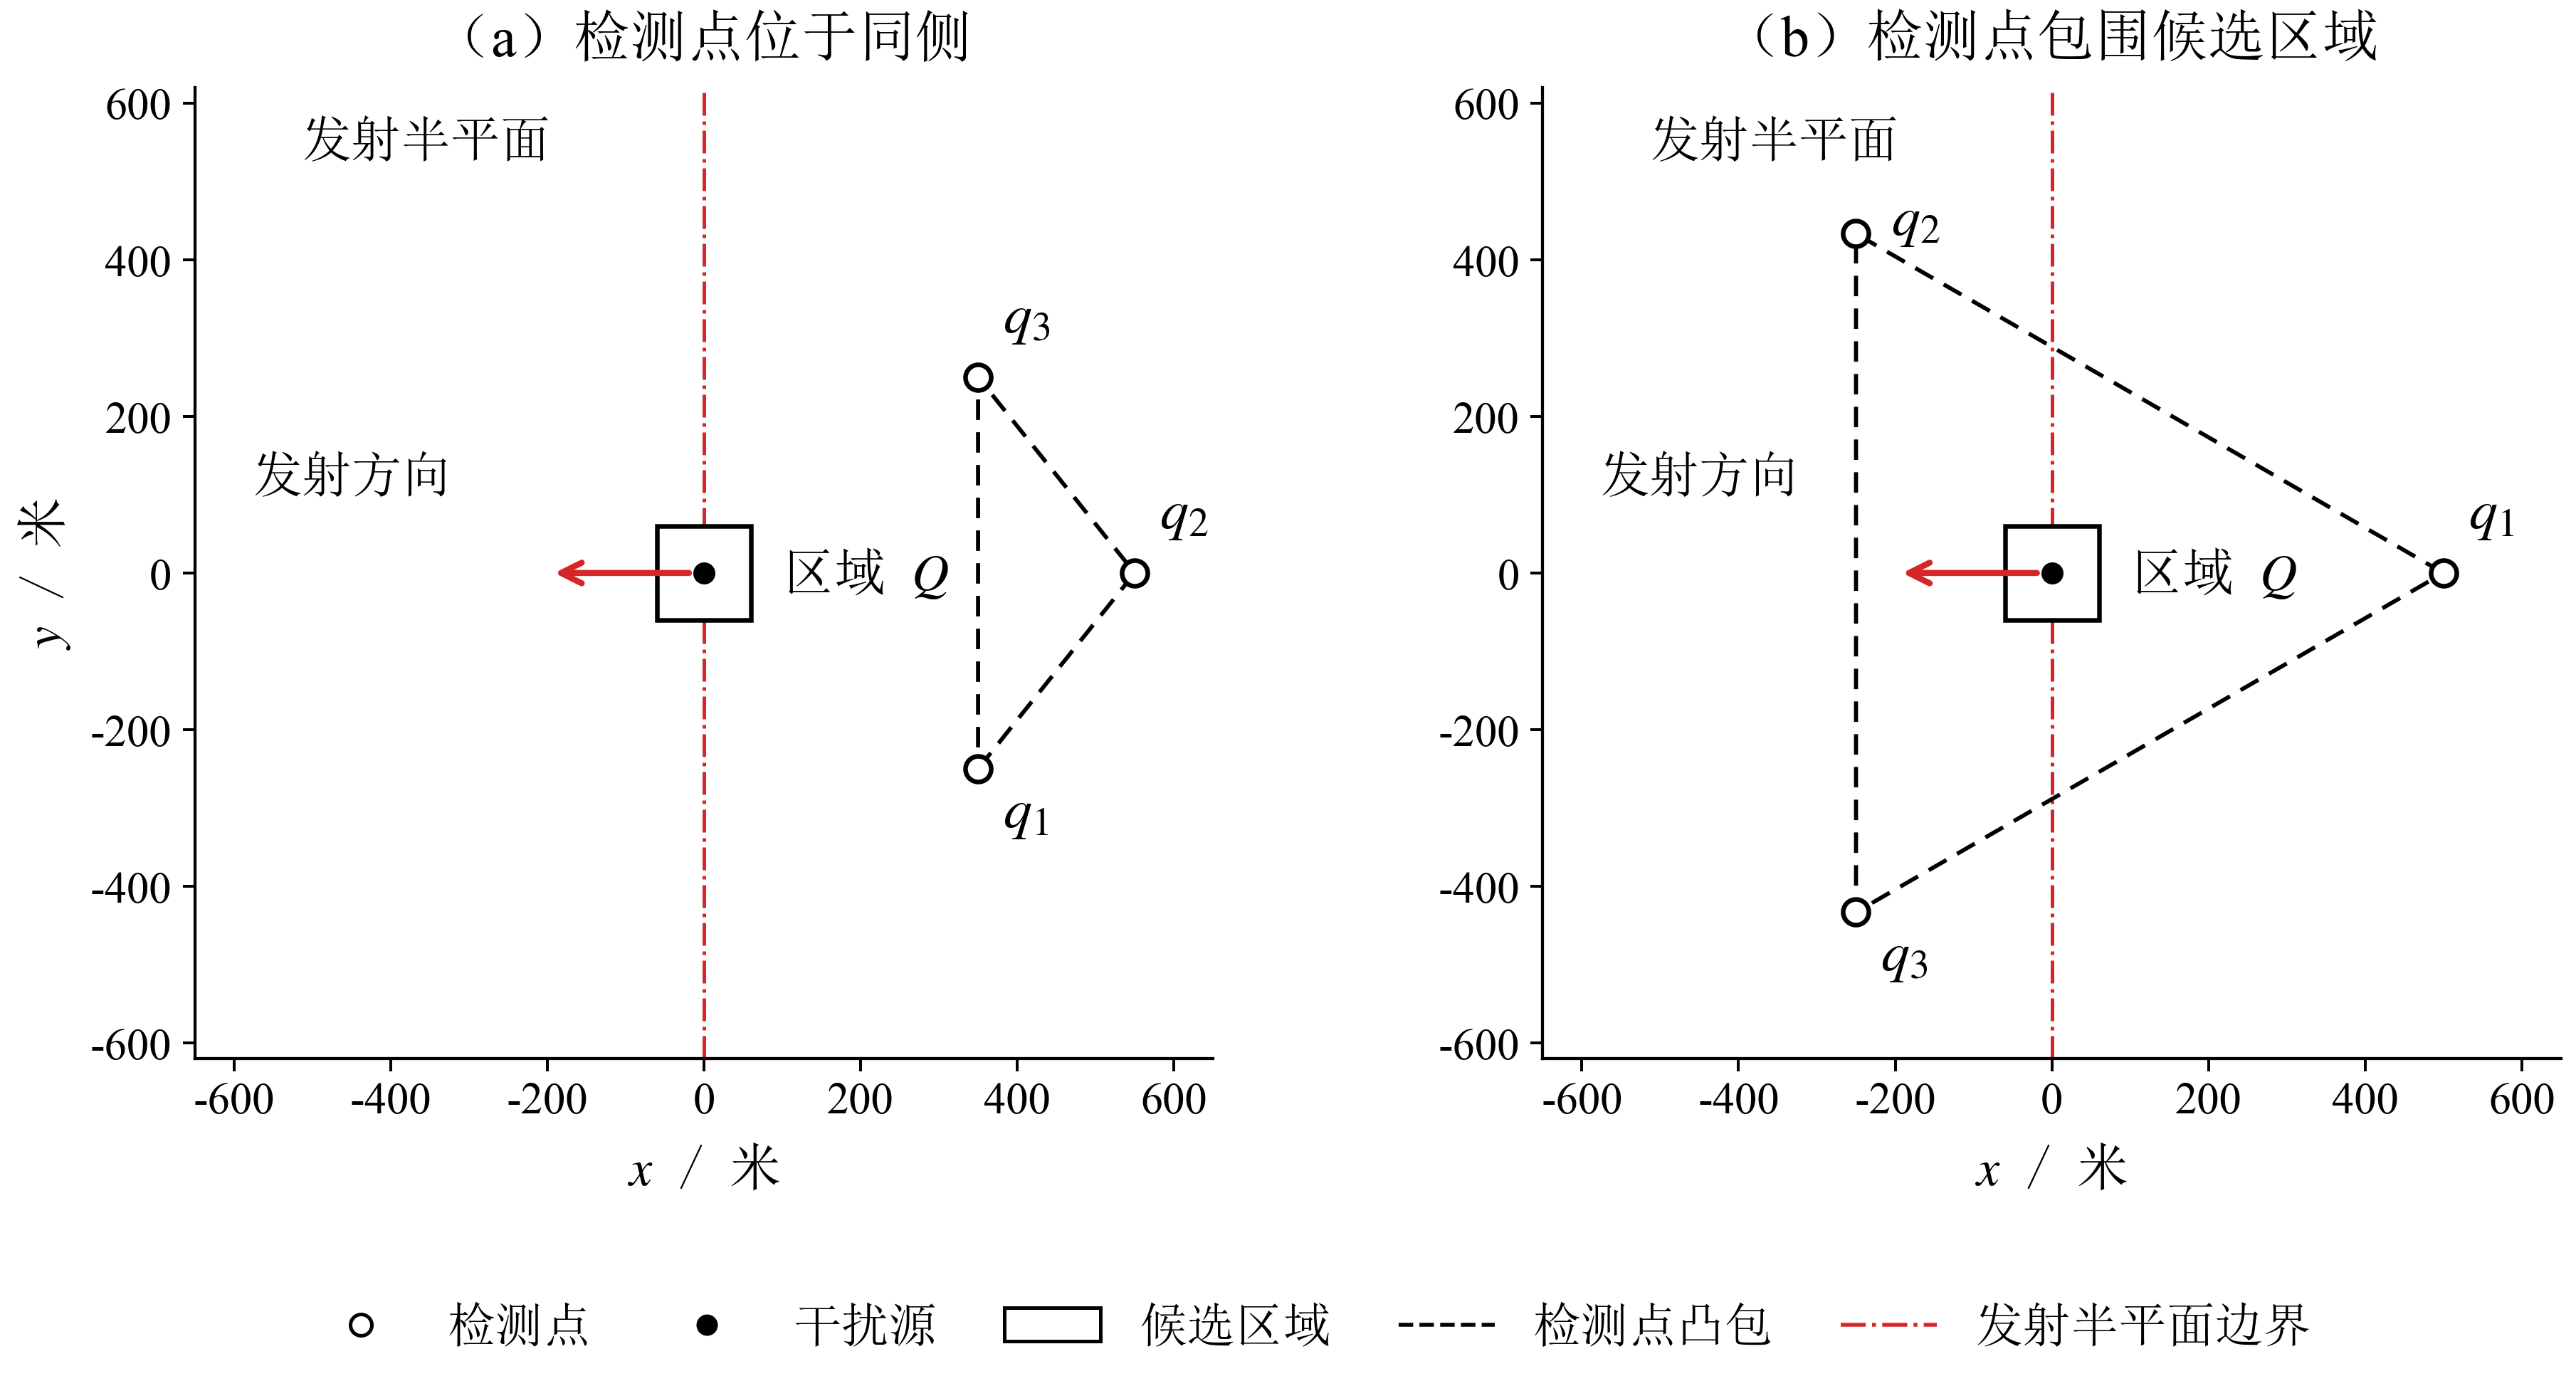
\includegraphics[width=0.96\linewidth,height=0.68\textheight,keepaspectratio]{figures/q4_directional_detection.png}
\caption{单侧检测与包围检测的方向覆盖}\label{fig:old5}
\end{figure}

设 \(Q\) 为候选源区域，\(P_Q\) 为检测点集合。我们要求：
\[
\max_{s\in P_Q}\sup_{g\in Q}\|s-g\|_2<R_{\min},
\qquad Q\subset\operatorname{int}\operatorname{conv}(P_Q),
\qquad R_{\min}=1000\ \text{米}
\tag{36}
\]

第一项保证检测点均在接收半径内，第二项保证检测点包围整个候选区域。式（36）给出与源朝向无关的排除充分条件，具体证明如下。

\begin{propositionbox}
\noindent 命题： 若 \(Q\) 与 \(P_Q\) 满足式（36），且同一频道在各检测点均实际返回无信号，则 \(Q\) 内不存在该频道当前未清除的源。

\noindent 证明： 假设存在源 \(g\in Q\)，全部检测点均在其接收半径内。全向源应被接收，与反馈矛盾；对朝向为 \(\boldsymbol d\) 的定向源，若所有检测点均处于 \(\boldsymbol d^{\mathsf T}(s-g)\le0\) 的半平面，其凸包也在该半平面内，边界上的 \(g\) 不能成为凸包内点，与式（36）矛盾。因此至少一个检测点满足 \(\boldsymbol d^{\mathsf T}(s-g)>0\)，应取得信号，同样与反馈矛盾。得证。
\end{propositionbox}

该条件同时约束后续检测位置。沿用第三问的无信号检测点集合 \(H^-_{c,t}\)、计划检测点集合 \(\mathcal P_{c,t}\) 和未排除区域 \(U_{c,t}\)。对每个潜在位置 \(g\)，从已执行与计划检测点中选出距离足够近的点，要求：
\[
\begin{aligned}
P_{c,t}(g)&=\{s\in H^-_{c,t}\cup\mathcal P_{c,t}:\|s-g\|_2<R_{\min}\},\\
g&\in\operatorname{int}\operatorname{conv}P_{c,t}(g),
\qquad \forall g\in U_{c,t},\ c\in\mathcal N_t
\end{aligned}
\tag{37}
\]

由上述命题可知，若式（37）成立，且相关检测均已完成并返回无信号，则 \(U_{c,t}\) 中不存在频道 \(c\) 未清除的源，可据此完成剩余排查。

终止条件沿用式（27）：已发现源全部清除，且未知频道的候选区域全部排空。

完整排查条件确定了怎样结束任务，路线选择则决定取得这些检测结果所需的时间。我们以式（37）替换第三问式（26）的圆盘覆盖约束，沿用式（28）---（30）的行动代价、完整退出时间及其期望最小化目标。累计时间包括最后一次清除后继续排查的耗时。

\subsection{模型的滚动求解}

\subsubsection{检测点生成与任务安排}

我们将剩余区域划分为可细分的凸多边形，逐块检验式（36）。对每块选定同一组检测点，检查全部顶点到这些点的距离及顶点是否位于其凸包内部。由凸性，顶点满足条件可保证整块区域满足条件；未通过检验的部分继续细分或保留。

初始巡测后，从满足式（37）的候选布局中选择计划检测点。执行巡测任务前，尝试将检测点移向现有路线或附近目标，仅接受保持式（37）且缩短路程的调整；删除检测点也须保持该条件。这样，已发现目标能够影响后续站位，剩余区域仍保留完整的检测安排。

巡测与已发现源的定位清除共同进入路线。巡测任务以检测点为代表位置，目标任务以当前定位区域的最小包围圆圆心为代表位置；定位区域较大且后续巡测可补充观测的目标暂缓访问，仍保留在待清除集合中。访问目标时继续测向或尝试清除，清除失败则根据反馈更新位置范围。

\subsubsection{后续检测与路线代价估计}

不同访问次序会改变新源被发现的时刻，进而改变后续检测次数和定位绕行。为估计这部分代价，我们选取有限的参数组合 \(x=(g,R,\phi,\zeta)\)，组成 \(\widehat{\mathcal H}_t\)。每完成一站对未知频道的巡测，删除在该站本应可见的组合；剩余组合用于预测未知源在后续检测点的可见性。

记已发现源数为 \(k_t\)，组合保留比例为 \(r_t=|\widehat{\mathcal H}_t|/|\widehat{\mathcal H}_0|\)。以 \(r_t\) 近似单源尚未被发现的概率，在总源数10至16的范围内采用权重 \(w_n=\binom n{k_t}r_t^{n-k_t}\)，估计剩余源数及各巡测站的检测频道数：
\[
\begin{aligned}
\widehat M_t&=
\frac{\displaystyle\sum_{n=\max(10,k_t)}^{16}(n-k_t)w_n}
{\displaystyle\sum_{n=\max(10,k_t)}^{16}w_n},\\
\widehat u_j&=u_t-\widehat M_t\left(1-\frac{|\widehat{\mathcal H}_{j^-}|}{|\widehat{\mathcal H}_t|}\right)
\end{aligned}
\tag{38}
\]

其中，\(u_t\) 为当前未知频道数，\(\widehat{\mathcal H}_{j^-}\) 为路线到达第 \(j\) 个巡测站前尚未覆盖的组合，\(\widehat M_t\) 和 \(\widehat u_j\) 分别为预计剩余源数与该站预计检测频道数。组合为空时取 \(\widehat M_t=0\)、\(\widehat u_j=u_t\)；已发现16个源时取 \(\widehat M_t=0\)。这些数值仅参与路线比较，排查完成仍依据真实反馈判断。

设 \(\sigma\) 为从当前位置出发的任务路线，\(L_t(\sigma)\) 为依次访问任务代表位置的路程，\(\mathcal S(\sigma)\) 为其中的巡测任务，\(\eta\) 为途中补测方案。为比较各路线完成巡测和定位的代价，将移动、检测与定位绕行换算为秒，并计入补测的预计作用：
\[
\widehat T_t(\sigma,\eta)=\frac{L_t(\sigma)}5
+6\sum_{j\in\mathcal S(\sigma)}\widehat u_j
+\frac{\widehat L_{\mathrm{refine},t}(\sigma)}5
-\frac{B_t(\sigma,\eta)}{10}
\tag{39}
\]

其中，\(\widehat L_{\mathrm{refine},t}\) 根据沿途新可见的组合估计定位细化的附加路程。\(B_t\) 用于比较途中补测的定位改进与检测开销：每个目标的预计定位半径收缩上限取300米，扣除30米检测等效路程后求和。移动按5米/秒换算，巡测按检测与切频合计6秒/频道估计；补测改进乘权重 \(1/2\) 后换算为时间，得到 \(B_t/10\)。实际行动耗时仍按式（28）累计。

\subsubsection{路线选择}

我们采用迭代局部搜索启发式算法调整任务次序，并构造以不同巡测站为首任务的替代路线。对生成的有限路线与补测方案集合 \(\Sigma_t\)，选择：
\[
(\sigma_t^*,\eta_t^*)\in\arg\min_{(\sigma,\eta)\in\Sigma_t}\widehat T_t(\sigma,\eta)
\tag{40}
\]

\subsubsection{滚动求解步骤}

\textbf{Step 1　初始化并巡测。} 按第三问初始化位置与频道状态，设置候选参数组合，完成初始巡测，取得各频道的首批反馈。

\textbf{Step 2　生成当前任务。} 按8.2.1节生成满足式（37）的计划检测点，与已发现源的定位清除任务共同组成当前任务集合。

\textbf{Step 3　选择任务路线。} 利用迭代局部搜索及不同首站构造候选路线，按式（38）估计检测频道数、式（39）计算路线代价，由式（40）选出当前路线。

\textbf{Step 4　执行首项任务。} 巡测任务在保持式（37）的条件下调整检测点，并执行途中补测与站点检测；目标任务执行定位与清除。途中补测获得有效新信息时，转入Step 5。

\textbf{Step 5　更新检测信息。} 按8.1.1节更新已发现源的定位范围与频道状态，利用实际无信号记录及式（36）更新未排除区域；一站未知频道巡测完成后，删除在该站本应可见的候选参数组合。

\textbf{Step 6　判断是否结束。} 满足式（27）时退出，并按式（29）记录完整耗时；否则返回Step 2。已发现源清除完毕而未知频道仍有未排除区域时，继续巡测。

\subsection{实验验证}

参数确定后，我们使用500个新随机种子检验完整退出情况与耗时。场景按演练分布生成，测向误差采用按频道区分的固定平滑空间场。源真值仅供运行结束后的评价；每源耗时先以各例完整退出时间除以该例原始源数，再跨例统计。结果见表\ref{tab:old8}。

\begingroup
\small
\setlength{\tabcolsep}{4pt}
\setlength{\TableInnerWidth}{\dimexpr\linewidth-2\tabcolsep\relax}
\renewcommand{\arraystretch}{1.22}
\begin{longtable}{@{}>{\centering\arraybackslash}p{0.700\TableInnerWidth}>{\centering\arraybackslash}p{0.300\TableInnerWidth}@{}}
\caption{独立500例的运行结果}\label{tab:old8}\\
\toprule
指标 & 结果 \\
\midrule
\endfirsthead
\multicolumn{2}{c}{表\thetable\quad 独立500例的运行结果（续）}\\
\toprule
指标 & 结果 \\
\midrule
\endhead
\midrule
\multicolumn{2}{r}{续下页}\\
\endfoot
\bottomrule
\endlastfoot
全清且正常退出案例数 & 500 \\
剩余源总数 & 0 \\
平均完整退出时间 / 秒 & 5282.57 \\
平均每源耗时 /（秒/源） & 416.13 \\
每源耗时95\%分位数 /（秒/源） & 556.07 \\
\end{longtable}
\endgroup

500例均完成全部清除并正常退出，统计时间包含失败清除与末段排查。图\ref{fig:old6}显示，每源耗时中位数为405.21秒/源，中间50\%的案例位于356.73至480.41秒/源。按相同口径统计，移动耗时为306.20秒/源，占总耗时约73.6\%，是本组测试的主要时间开销。

\begin{figure}[H]
\centering
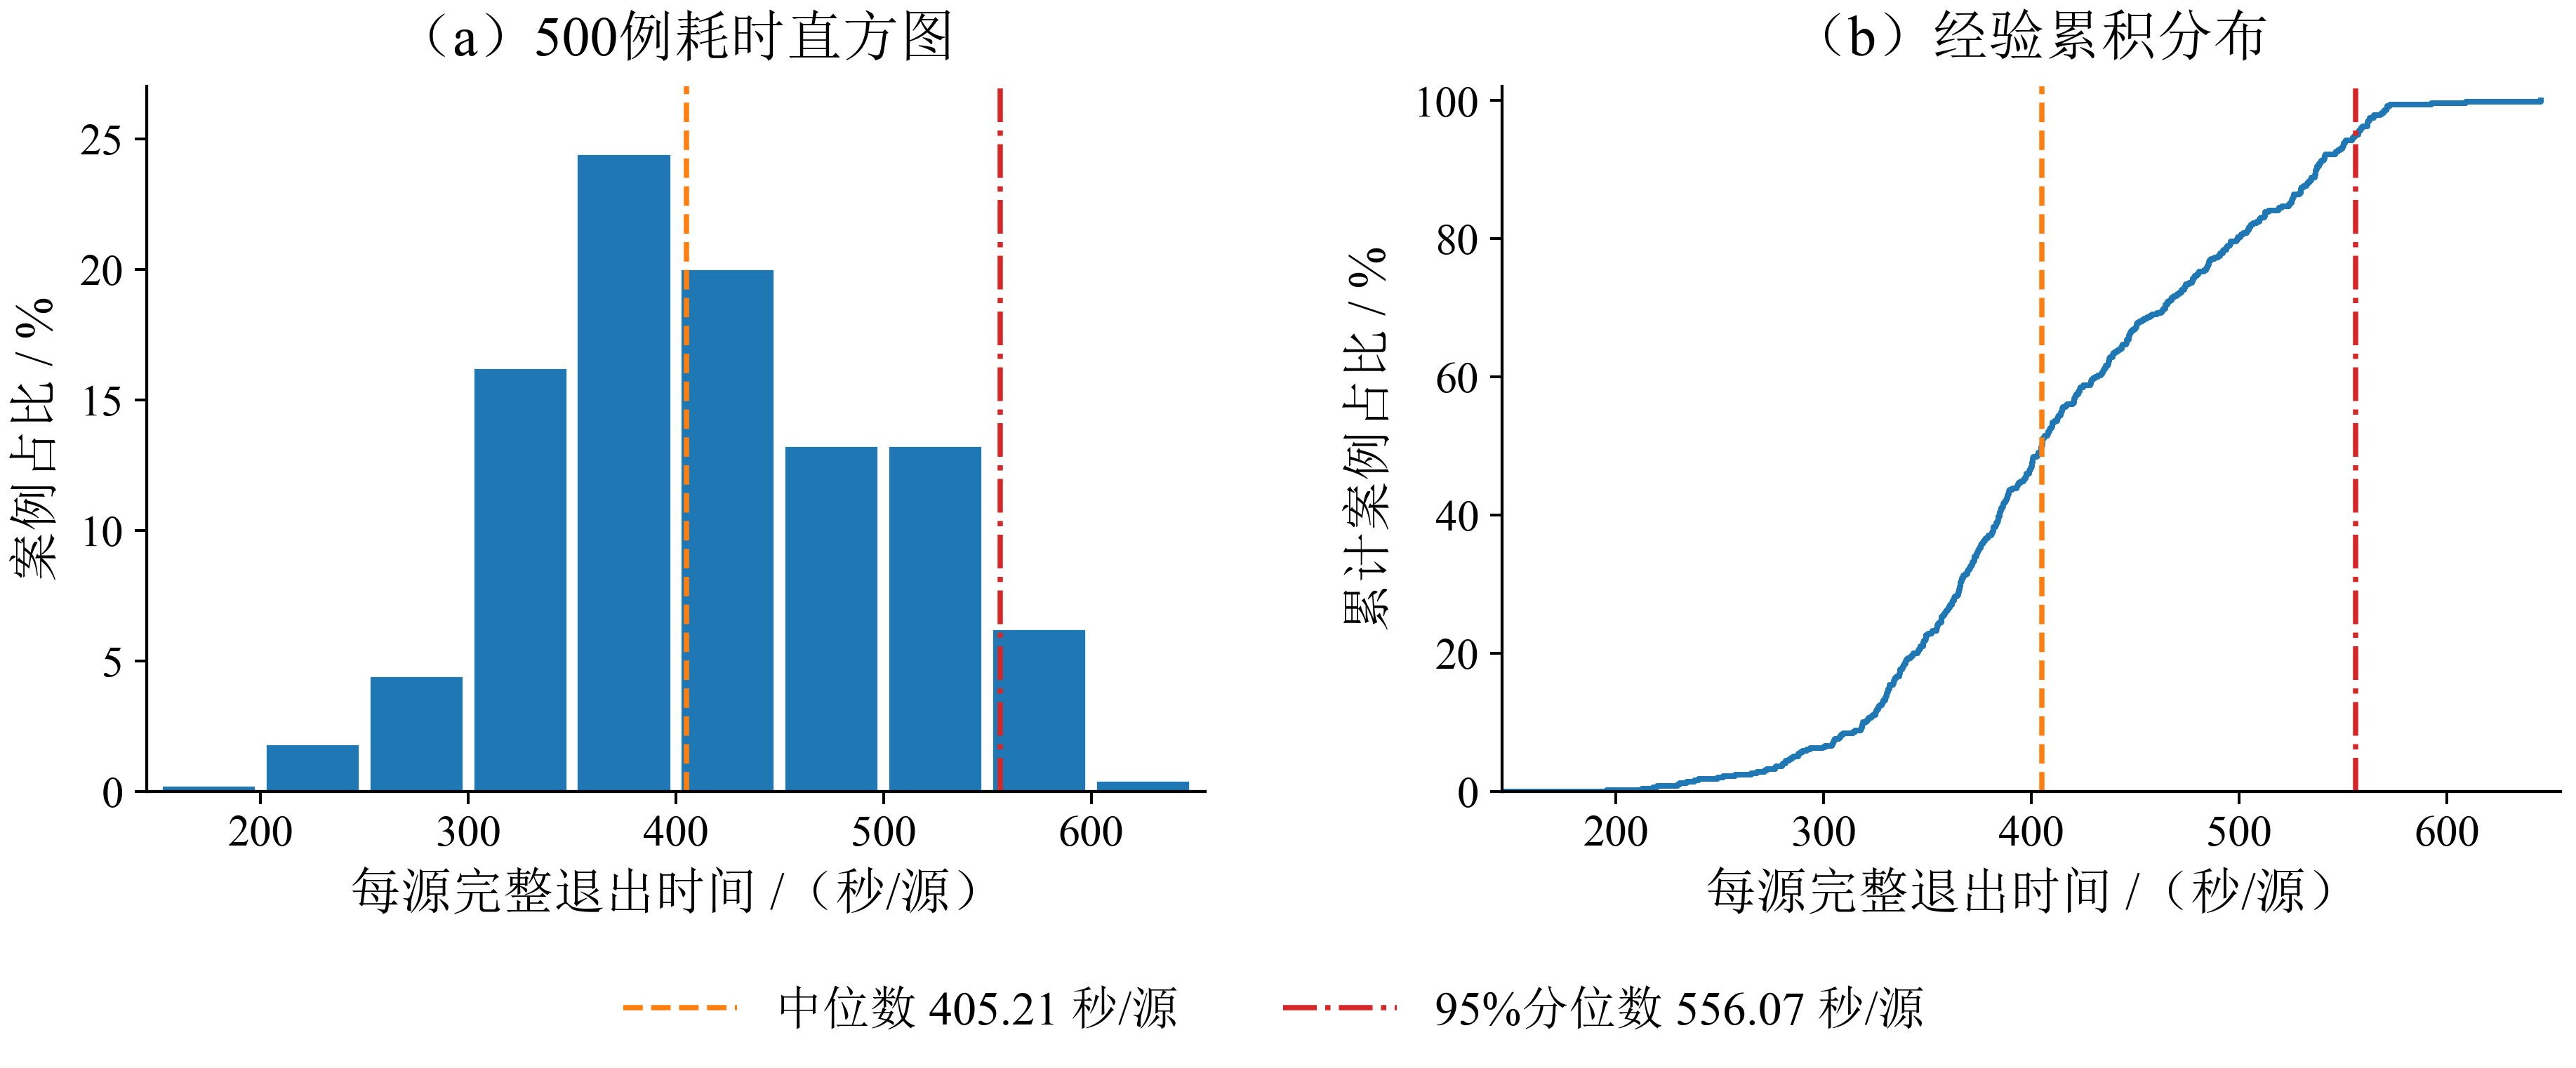
\includegraphics[width=0.96\linewidth,height=0.68\textheight,keepaspectratio]{figures/q4_time_distribution500.png}
\caption{第四问每源完整退出耗时的经验分布}\label{fig:old6}
\end{figure}

图\ref{fig:q4-example-traces}展示此前200例验证中两个案例的完整轨迹。灰线表示巡测与清除，蓝线表示最后清除后的排查，蓝色方形标示退出位置。两例均清除了全部13个源，末段排查分别耗时115.10秒和86.48秒。源位置采用运行结束后的真值。

\begin{figure}[H]
\centering
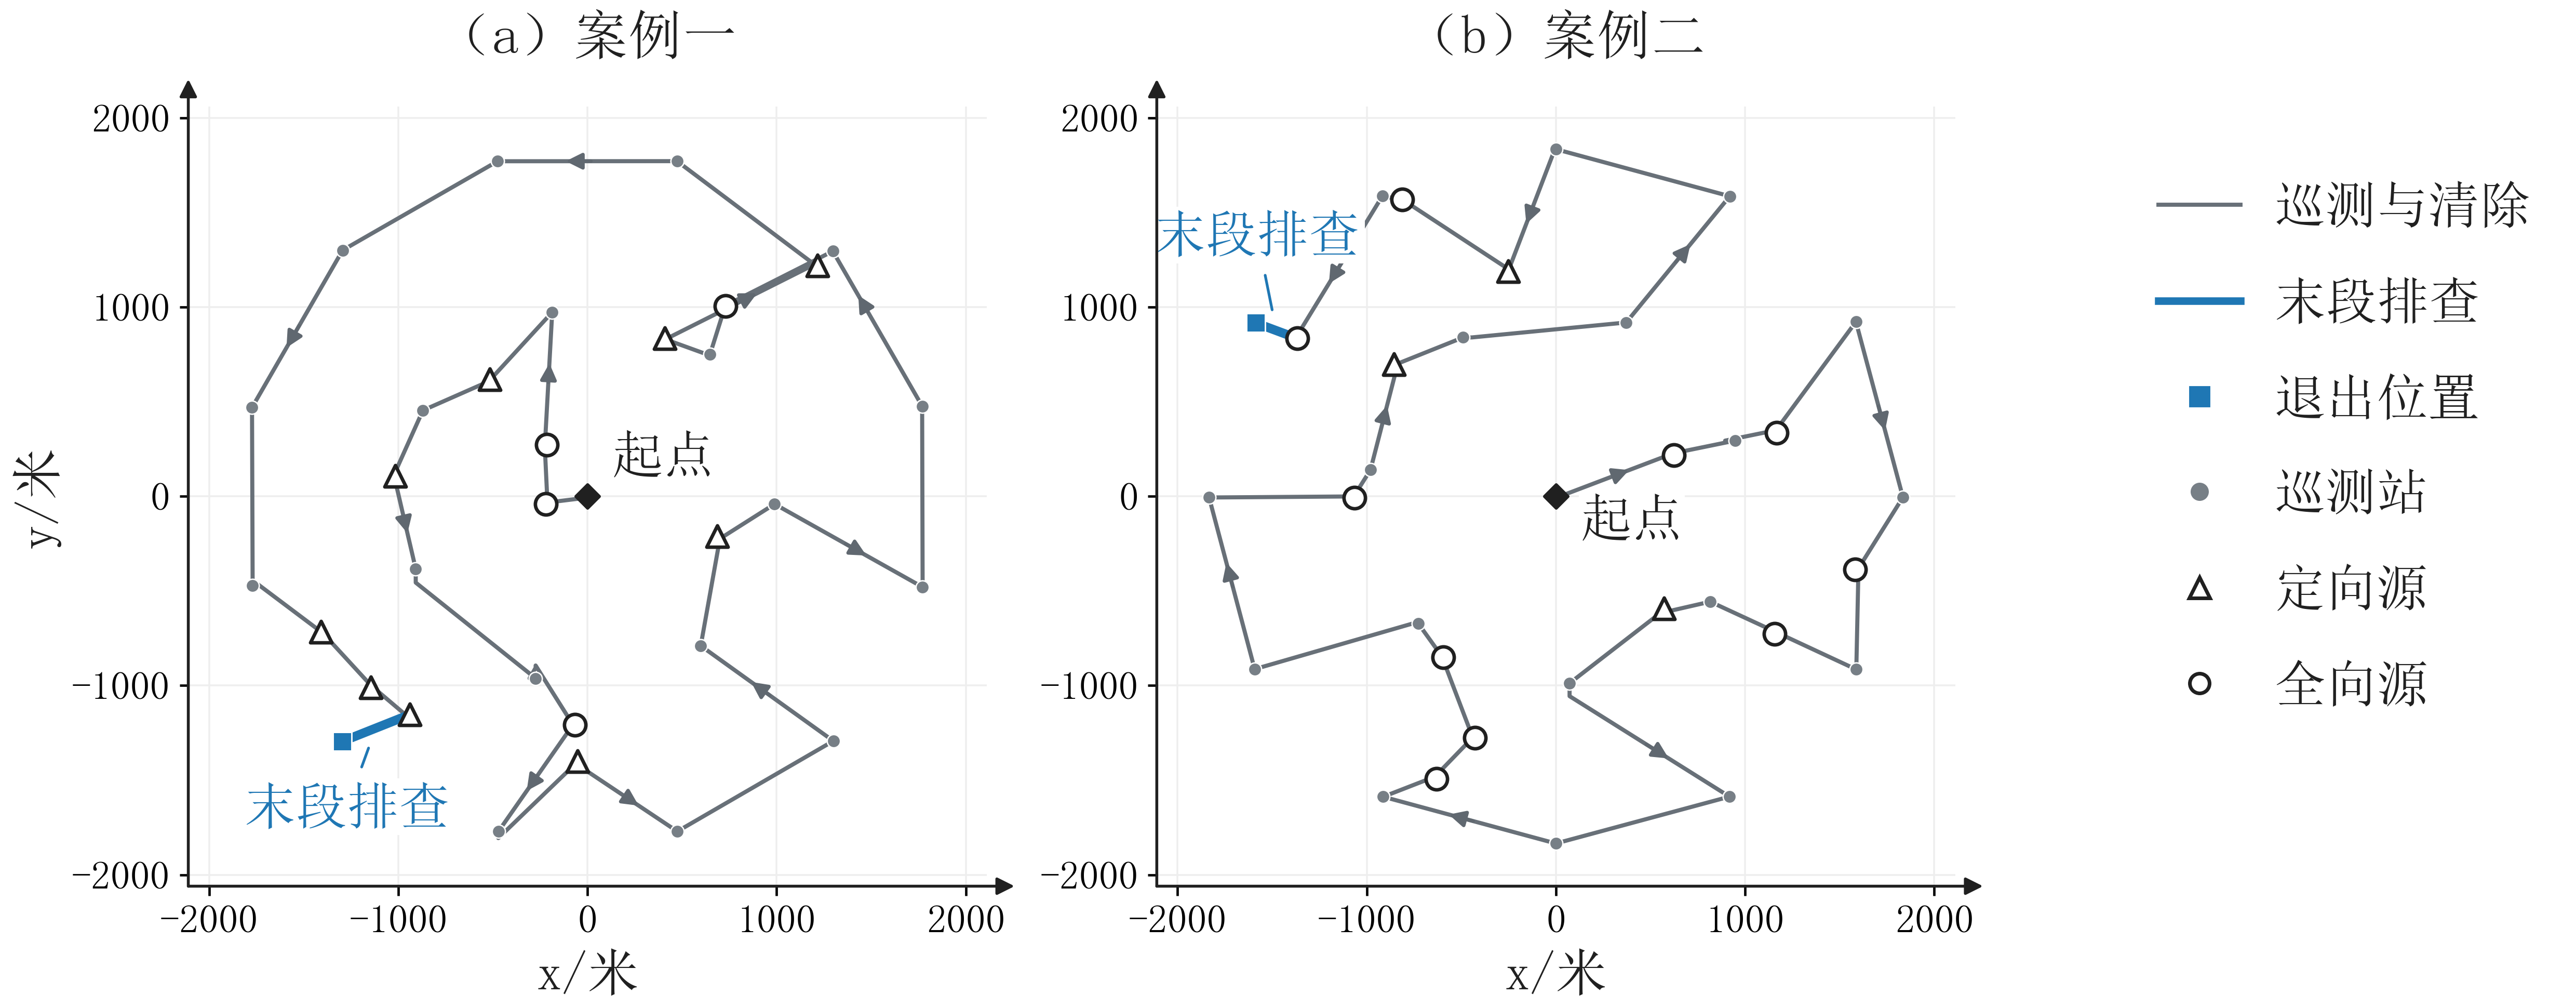
\includegraphics[width=0.99\linewidth,keepaspectratio]{figures/q4_example_trace_cases.png}
\caption{两个案例的完整行动轨迹}\label{fig:q4-example-traces}
\end{figure}

\Needspace{12\baselineskip}
\subsection{正式测试结果}

第四问的三次正式测试均清除了全部干扰源，结果见表\ref{tab:old9}，两项时间分别按第三问正式测试中的虚拟任务耗时与现实执行时长统计。

\begin{table}[H]
\centering
\small
\setlength{\tabcolsep}{4pt}
\setlength{\TableInnerWidth}{\dimexpr\linewidth-6\tabcolsep\relax}
\renewcommand{\arraystretch}{1.22}
\caption{问题4正式测试结果}\label{tab:old9}
\begin{tabular}{@{}>{\centering\arraybackslash}p{0.390\TableInnerWidth}>{\centering\arraybackslash}p{0.170\TableInnerWidth}>{\centering\arraybackslash}p{0.260\TableInnerWidth}>{\centering\arraybackslash}p{0.180\TableInnerWidth}@{}}
\toprule
测试案例编码 & 清除干扰源个数 & 平均定位清除时间 /（秒/源） & 程序运行时间 / 秒 \\
\midrule
XH33-K2C8-8MEP-YJYN & 15 & 335.286 & 6.373 \\
2VV2-BRDE-U2HD-F5PU & 11 & 498.589 & 6.543 \\
CPE4-6NCH-EFMC-8RVG & 10 & 542.428 & 5.932 \\
\bottomrule
\end{tabular}
\end{table}

\subsection{灵敏度分析与消融实验}

开发集与独立验证集各取100个随机种子，各设置按同种子配对。独立验证中，四种设置均完成全部清除并正常退出，结果见表\ref{tab:q4-sensitivity-ablation}。

\begingroup
\small
\setlength{\tabcolsep}{4pt}
\setlength{\TableInnerWidth}{\dimexpr\linewidth-4\tabcolsep\relax}
\renewcommand{\arraystretch}{1.12}
\begin{longtable}{@{}>{\centering\arraybackslash}p{0.450\TableInnerWidth}>{\centering\arraybackslash}p{0.330\TableInnerWidth}>{\centering\arraybackslash}p{0.220\TableInnerWidth}@{}}
\caption{补测权重与途中补测机制的独立验证结果}\label{tab:q4-sensitivity-ablation}\\
\toprule
实验设置 & 平均每源耗时 /（秒/源） & 相对基准变化 \\
\midrule
\endfirsthead
\multicolumn{3}{c}{表\thetable\quad 补测权重与途中补测机制的独立验证结果（续）}\\
\toprule
实验设置 & 平均每源耗时 /（秒/源） & 相对基准变化 \\
\midrule
\endhead
\midrule
\multicolumn{3}{r}{续下页}\\
\endfoot
\bottomrule
\endlastfoot
补测收益权重0.25 & 420.82 & -0.02\% \\
补测收益权重0.50（基准） & 420.89 & 0.00\% \\
补测收益权重1.00 & 420.08 & -0.19\% \\
关闭途中补测及奖励 & 425.62 & +1.12\% \\
\end{longtable}
\endgroup

（1）灵敏度分析。 将式（39）中的补测收益权重取0.25、0.50和1.00，平均每源耗时极差为0.81秒，仅占基准的0.19\%。两种权重变体分别有98例和96例与基准轨迹相同，权重调整对行动次序影响较小。

（2）消融实验。 关闭途中补测及其奖励后，平均每源耗时增加4.73秒，配对差的95\%自助置信区间为[2.24，7.55]秒。其中，移动耗时增加4.62秒/源，是新增代价的主要来源，表明途中补测减少了后续定位绕行。

\FloatBarrier
\section{模型评价}

\subsection{模型的优点}

（1）精度与可靠性：我们以有界示向度约束构造定位区域，以区域直径与最小包围圆半径度量其跨度与最坏预测误差。该度量不借助误差的分布假设；最小包围圆同时给出预测位置与误差上界，二者分别是圆心与半径。当半径不超过 20 米时，圆心落入保证清除区域；该上界不随误差分布而变，反映了模型的可靠定位精度。

（2）通用性：我们构建的第二检测点选址模型以接收范围与观测几何作为选点准则，将近距离、方向与无信号三类反馈纳入同一模型。配对测试中，按该模型选点所得预测误差远低于随机选点。三类反馈与不同观测几何共用一套选点准则，选点过程不因反馈类型而更换模型形式。

（3）任务完备性：我们将未知频道巡测、已发现源的补充定位与清除纳入同一任务集合，三者共享同一行动次序并随反馈更新。终止条件同时检查已清除结果与未知频道的剩余区域，任务在两者均无剩余时结束。基于该终止条件，第三、四问的独立测试均完成全部清除并正常退出，清除与排查两类目标均无遗留，完整地完成了既定任务。

（4）可解释性：针对未知发射朝向，我们将接收半径下界与检测点凸包的包围关系结合，给出与源朝向无关的区域排除充分条件。该条件只用检测点位置与接收半径下界两个几何量判定，不含源朝向的估计；检测点调整与路线优化据此始终受完整排查条件约束。判定不依赖统计推断，排除与否可直接由检测点与源的几何关系说明，解释性强。

\subsection{模型的不足}

（1）准则保守性：基于上述最坏情形准则，第二问依据最不利反馈选择检测位置，常见反馈下的平均误差未纳入选点准则。第四问同样以充分条件约束整块区域，要求同一组检测点满足距离与包围关系，该条件会保留部分尚可排除的区域。两部分保守性叠加，巡测工作量因此增加；细化边界区域可缓解这一影响，准则的保守性仍是定位策略的主要代价。

（2）离散近似：第二问采用位置网格加密与方向反馈枚举，第三、四问以有限场景、参数组合及候选路线近似未来任务。这些离散与近似使连续模型的全局最优性无法直接沿用，解的质量仍取决于网格与候选集的规模。

（3）条件依赖：定位模型以源位置固定、检测点坐标准确与示向度误差有界为基础前提。模拟检验采用演练分布与固定平滑误差场，所得精度与耗时只对应这一组测试条件。模型迁移到真实场景时先标定测量误差与接收范围，再检验覆盖情况与任务完成率；所得结果取决于这些前提在真实场景中的成立程度。


\section*{AI工具使用声明}
本参赛队在竞赛过程中使用了DeepSeek V4.1 Flash，辅助完成资料与文献整理、程序调试、数据与图表整理、文字润色、排版及支撑材料整理。采纳内容经本参赛队核验，具体使用过程与核验情况见支撑材料中的《AI工具使用详情》。


\begin{thebibliography}{7}
\bibitem{ref1}
TOKEKAR P, ISLER V. Sensor placement and selection for bearing sensors with bounded uncertainty[C]//2013 IEEE International Conference on Robotics and Automation. IEEE, 2013: 2515–2520. DOI: \href{https://doi.org/10.1109/ICRA.2013.6630920}{\nolinkurl{10.1109/ICRA.2013.6630920}}.

\bibitem{ref2}
VANDER HOOK J, TOKEKAR P, ISLER V. Cautious greedy strategy for bearing-only active localization: Analysis and field experiments[J]. Journal of Field Robotics, 2014, 31(2): 296–318. DOI: \href{https://doi.org/10.1002/rob.21499}{\nolinkurl{10.1002/rob.21499}}.

\bibitem{ref3}
JIANG H, CAI Y, YU Z. Observability metrics for single-target tracking with bearings-only measurements[J]. IEEE Transactions on Systems, Man, and Cybernetics: Systems, 2022, 52(2): 1065–1077. DOI: \href{https://doi.org/10.1109/TSMC.2020.3012485}{\nolinkurl{10.1109/TSMC.2020.3012485}}.

\bibitem{ref5}
LI Y, QI G, SHENG A. Optimal deployment of vehicles with circular formation for bearings-only multi-target localization[J]. Automatica, 2019, 105: 347–355. DOI: \href{https://doi.org/10.1016/j.automatica.2019.04.008}{\nolinkurl{10.1016/j.automatica.2019.04.008}}.

\bibitem{ref4}
RUAN T, HUANG Y, ZHU Q, et al. Multi-stage RF emitter search and geolocation with UAV: A cognitive learning-based method[J]. IEEE Transactions on Vehicular Technology, 2023, 72(5): 6349–6362. DOI: \href{https://doi.org/10.1109/TVT.2023.3235498}{\nolinkurl{10.1109/TVT.2023.3235498}}.

\bibitem{ref7}
ZHAO Y, CHEN B, WANG X, et al. A deep reinforcement learning based searching method for source localization[J]. Information Sciences, 2022, 588: 67–81. DOI: \href{https://doi.org/10.1016/j.ins.2021.12.041}{\nolinkurl{10.1016/j.ins.2021.12.041}}.

\bibitem{ref6}
WANG Y, CAO G. On full-view coverage in camera sensor networks[C]//2011 Proceedings IEEE INFOCOM. IEEE, 2011: 1781–1789. DOI: \href{https://doi.org/10.1109/INFCOM.2011.5934977}{\nolinkurl{10.1109/INFCOM.2011.5934977}}.

\end{thebibliography}


\clearpage
\appendix
\renewcommand{\thesection}{附录\Alph{section}}
\renewcommand{\thesubsection}{\Alph{section}.\arabic{subsection}}
\clearpage\section{问题一算法的复杂度与优化}\label{appendix-a}

\subsection{算法的计算量}

每次测向产生两个半平面约束，\(m\) 次观测共给出 \(2m\) 条边界。算法1枚举边界对，候选交点数量至多为 \(\binom{2m}{2}\)；每个交点需要代入全部 \(2m\) 个约束进行检验，因此顶点枚举阶段的计算量为 \(O(m^3)\)。该估计针对边界求交与约束校验，不包含可行性及有界性判别所调用的线性规划求解器的内部计算。

得到 \(h\) 个顶点后，枚举顶点对计算直径的计算量为 \(O(h^2)\)，检验直径圆是否覆盖全部顶点的计算量为 \(O(h)\)。对于由 \(2m\) 个半平面构成的有界凸多边形，\(h\le2m\)，因此这两个步骤不改变顶点枚举部分的立方级计算量。

\subsection{检测点较多时的优化}

当检测点数量较多时，可将边界对枚举替换为按方向排序的半平面求交。先将半平面按边界方向排序，再用双端队列维护有效边界：同向平行约束保留较严格者，新约束加入时从队列两端删除与之不相容的边界。排序需要 \(O(m\log m)\) 的计算量，每条边界至多入队和出队一次，后续维护为线性计算量；空集、无界及退化情形仍须分别判别。

对求得的有界凸多边形，可进一步采用旋转卡壳法，沿有序顶点遍历对踵点对，在 \(O(h)\) 的计算量内求出直径，再按正文判据检验覆盖性。这样，半平面求交与直径计算这两个主要几何步骤可达到 \(O(m\log m)\) 的总计算复杂度。

正文算例使用的是边界对枚举实现。本节所述排序求交与旋转卡壳属于可选优化方案，尚未用于所报告的实验，因此不据此作出实际运行时间已经缩短的结论。

\clearpage\section{粗网格与局部增密搜索算法伪代码}\label{appendix-b}

\begin{pseudocodetable}
\begin{longtable}{@{}>{\raggedleft\arraybackslash}p{1.8em}@{\hspace{0.65em}}>{\raggedright\arraybackslash}p{\AlgorithmTextWidth}@{}}
\toprule
\multicolumn{2}{@{}p{\linewidth}@{}}{\textbf{算法 2}\quad 粗网格与局部增密搜索算法}\\
\midrule
\multicolumn{2}{@{}p{\linewidth}@{}}{\textbf{输入：}首次检测点 \(s_1\)，示向度 \(\theta_1\)，题设常量，容许误差增量 \(\Delta\)}\\
\multicolumn{2}{@{}p{\linewidth}@{}}{\textbf{输出：}近优候选集 \(\widehat{\mathcal C}_\Delta\)，各候选评分，代表检测点 \(s^*\)}\\
\endfirsthead
\toprule
\multicolumn{2}{@{}p{\linewidth}@{}}{\textbf{算法 2}\quad 粗网格与局部增密搜索算法（续）}\\
\midrule
\endhead
\midrule
\multicolumn{2}{r}{续下页}\\
\endfoot
\bottomrule
\endlastfoot
\addlinespace[3pt]
1. & \AlgorithmStep{0}{按式(9)构造 \(F_1\)；若为空，返回“观测不相容”}\\
2. & \AlgorithmStep{0}{按式(18)确定搜索外包域 \(\mathcal S\)，在域内生成粗网格}\\
3. & \AlgorithmStep{0}{\(V\gets\varnothing\)}\\
4. & \AlgorithmStep{0}{逐级执行位置搜索}\\
5. & \AlgorithmStep{1.2}{遍历本级每个待评价位置 \(s\)}\\
6. & \AlgorithmStep{2.4}{若 \(s=s_1\)，令评分为 \(\rho(F_1)\)}\\
7. & \AlgorithmStep{2.4}{否则按式(13a)至式(13c)计算近距离、无信号分支，并枚举方向反馈}\\
8. & \AlgorithmStep{3.6}{排除不可能反馈，对其余位置集合计算最小包围圆半径}\\
9. & \AlgorithmStep{3.6}{取各反馈半径的最大值，得到 \(\widehat J(s)\)}\\
10. & \AlgorithmStep{2.4}{保存位置、评分及最坏反馈，加入 \(V\)}\\
11. & \AlgorithmStep{1.2}{在低评分候选附近生成下一层增密网格}\\
12. & \AlgorithmStep{0}{以统一精度增密复核拟用于输出的候选，将这批候选重新记为 \(V\)}\\
13. & \AlgorithmStep{0}{\(\widehat J_{\text{基准}}\gets\) 候选集 \(V\) 中的评分最小值}\\
14. & \AlgorithmStep{0}{\(\widehat{\mathcal C}_\Delta\gets\{v\in V:\widehat J(v)\le\widehat J_{\text{基准}}+\Delta\}\)}\\
15. & \AlgorithmStep{0}{从评分最小的候选中取代表点 \(s^*\)，返回结果}\\
\end{longtable}
\end{pseudocodetable}

\clearpage
\section{支撑材料文件列表}
精简支撑材料共48个文件，包含32个源程序与6个官方正式测试日志。以下路径相对于压缩包根目录，运行方法见\path{README.md}。
\begingroup
\fontsize{8.5}{11}\selectfont
\renewcommand{\arraystretch}{1.0}
\setlength{\tabcolsep}{3pt}
\setlength{\LTpre}{3pt}
\setlength{\LTpost}{3pt}
\par\needspace{5\baselineskip}\noindent\textbf{目录：}根目录
\begin{longtable}{@{}p{0.67\linewidth}p{0.28\linewidth}@{}}
\toprule 文件名 & 用途 \\ \midrule
\endfirsthead
\toprule 文件名 & 用途 \\ \midrule
\endhead
\bottomrule\endfoot
\path{AI}工具使用详情\path{.pdf} & AI使用详情核对稿 \\
\path{README.md} & 阅读与运行说明 \\
\path{requirements.txt} & Python依赖 \\
\end{longtable}
\par\needspace{5\baselineskip}\noindent\textbf{目录：}\path{q1}
\begin{longtable}{@{}p{0.67\linewidth}p{0.28\linewidth}@{}}
\toprule 文件名 & 用途 \\ \midrule
\endfirsthead
\toprule 文件名 & 用途 \\ \midrule
\endhead
\bottomrule\endfoot
\path{cases.json} & 第一问输入、预设几何与结果 \\
\path{q1_geometry.py} & 第一问几何求解 \\
\end{longtable}
\par\needspace{5\baselineskip}\noindent\textbf{目录：}\path{q2}
\begin{longtable}{@{}p{0.67\linewidth}p{0.28\linewidth}@{}}
\toprule 文件名 & 用途 \\ \midrule
\endfirsthead
\toprule 文件名 & 用途 \\ \midrule
\endhead
\bottomrule\endfoot
\path{benchmark_helpers.py} & 第二问观测模拟与三规则求解 \\
\path{geometry_snapshot.py} & 第二问几何运算 \\
\path{policies.py} & 观测更新与选点规则 \\
\path{practice_snapshot.py} & 演练生成与误差场 \\
\path{results.jsonl} & 第二问5000例种子与结果 \\
\end{longtable}
\par\needspace{5\baselineskip}\noindent\textbf{目录：}\path{q2/search}
\begin{longtable}{@{}p{0.67\linewidth}p{0.28\linewidth}@{}}
\toprule 文件名 & 用途 \\ \midrule
\endfirsthead
\toprule 文件名 & 用途 \\ \midrule
\endhead
\bottomrule\endfoot
\path{check_finalists.py} & 第二问候选点精细角度搜索 \\
\path{compare.py} & 候选点搜索与比较 \\
\path{geometry.py} & 几何运算 \\
\path{model_snapshot.py} & 第二问选点损失模型 \\
\path{result.json} & 第二问候选点与精细角度搜索结果 \\
\end{longtable}
\par\needspace{5\baselineskip}\noindent\textbf{目录：}\path{q3}
\begin{longtable}{@{}p{0.67\linewidth}p{0.28\linewidth}@{}}
\toprule 文件名 & 用途 \\ \midrule
\endfirsthead
\toprule 文件名 & 用途 \\ \midrule
\endhead
\bottomrule\endfoot
\path{action_timing.py} & 动作时间定义 \\
\path{bearing_correlation.py} & 空间误差相关处理 \\
\path{cli.py} & 第三问命令行入口 \\
\path{client.py} & HTTP协议与记录 \\
\path{coverage_geometry.py} & 第三问覆盖几何 \\
\path{geometry.py} & 几何运算 \\
\path{local_simulator.py} & 本地演练模拟器 \\
\path{moving_stations.py} & 移动检测候选生成 \\
\path{practice_reference.py} & 演练分布生成 \\
\path{results.jsonl} & 第三问1000例种子与结果 \\
\path{robot.py} & 第三问滚动决策 \\
\path{rotate_selector.py} & 覆盖布局旋转选择 \\
\path{rotation-layouts.json} & 第三问覆盖布局 \\
\path{sampled_recourse.py} & 条件场景后续代价 \\
\path{tail_lens.py} & 末段定位候选 \\
\end{longtable}
\par\needspace{5\baselineskip}\noindent\textbf{目录：}\path{q4}
\begin{longtable}{@{}p{0.67\linewidth}p{0.28\linewidth}@{}}
\toprule 文件名 & 用途 \\ \midrule
\endfirsthead
\toprule 文件名 & 用途 \\ \midrule
\endhead
\bottomrule\endfoot
\path{belief.py} & 第四问位置与方向状态 \\
\path{coverage.py} & 第四问覆盖证明读取与排查 \\
\path{coverage_proofs.json.gz} & 第四问覆盖证书数据 \\
\path{entry.py} & 第四问运行入口 \\
\path{geometry.py} & 几何运算 \\
\path{gridline.py} & 第四问检测布局 \\
\path{local_simulator.py} & 本地演练模拟器 \\
\path{practice_reference.py} & 演练分布生成 \\
\path{protocol.py} & HTTP协议与记录 \\
\path{results.jsonl} & 第四问500例种子与结果 \\
\path{routes.py} & 第四问路线候选 \\
\path{strategy.py} & 第四问滚动决策 \\
\end{longtable}
\par\needspace{5\baselineskip}\noindent\textbf{目录：}正式测试文件\path{/3}
\begin{longtable}{@{}p{0.67\linewidth}p{0.28\linewidth}@{}}
\toprule 文件名 & 用途 \\ \midrule
\endfirsthead
\toprule 文件名 & 用途 \\ \midrule
\endhead
\bottomrule\endfoot
\path{formal-p3-1-UJBC-A4W9-A6FZ-XYQF.jlog} & 第三问正式日志 \\
\path{formal-p3-2-CQFE-KMZK-43Z9-VC6H.jlog} & 第三问正式日志 \\
\path{formal-p3-3-5P3S-DMUG-M4NP-N8W4.jlog} & 第三问正式日志 \\
\end{longtable}
\par\needspace{5\baselineskip}\noindent\textbf{目录：}正式测试文件\path{/4}
\begin{longtable}{@{}p{0.67\linewidth}p{0.28\linewidth}@{}}
\toprule 文件名 & 用途 \\ \midrule
\endfirsthead
\toprule 文件名 & 用途 \\ \midrule
\endhead
\bottomrule\endfoot
\path{formal-p4-1-XH33-K2C8-8MEP-YJYN.jlog} & 第四问正式日志 \\
\path{formal-p4-2-2VV2-BRDE-U2HD-F5PU.jlog} & 第四问正式日志 \\
\path{formal-p4-3-CPE4-6NCH-EFMC-8RVG.jlog} & 第四问正式日志 \\
\end{longtable}
\endgroup

\clearpage
\section{完整源程序与运行命令}
以下列出精简支撑包中的完整源程序。展示时删去注释、说明性文档字符串和空白行，语句与运算保持不变。运行时使用支撑包中的源文件，保留其目录结构。
\begin{mdframed}[linewidth=0.45pt,linecolor=black,backgroundcolor=white,innerleftmargin=5pt,innerrightmargin=5pt,innertopmargin=4pt,innerbottommargin=4pt,skipabove=5pt,skipbelow=5pt,everyline=true]
\begin{Verbatim}[fontsize=\small,breaklines=true]
python -m pip install -r requirements.txt
python q1/q1_geometry.py
python q2/benchmark_helpers.py --count 10
python q3/robot.py demo --problem 3 --seed 20260910 --quiet
python q4/entry.py demo --problem 4 --seed 20260910 --quiet
python q2/search/compare.py
python q2/search/check_finalists.py
\end{Verbatim}
\end{mdframed}
\begingroup
\fvset{fontsize=\fontsize{8}{9.6}\selectfont,baselinestretch=1,numbers=left,numbersep=4pt,numberblanklines=false,breaklines=true,breakanywhere=true,breaksymbolleft={},breaksymbolright={},xleftmargin=12pt,tabsize=4}
\par\needspace{8\baselineskip}
\subsection*{程序 1：第一问几何求解}
\noindent \path{q1/q1_geometry.py}\par
\begin{mdframed}[linewidth=0.45pt,linecolor=black,backgroundcolor=white,innerleftmargin=5pt,innerrightmargin=5pt,innertopmargin=4pt,innerbottommargin=4pt,skipabove=5pt,skipbelow=5pt,everyline=true]
\VerbatimInput{appendix_code/q1/q1_geometry.py}
\end{mdframed}
\par\needspace{8\baselineskip}
\subsection*{程序 2：第二问观测模拟与三规则求解}
\noindent \path{q2/benchmark_helpers.py}\par
\begin{mdframed}[linewidth=0.45pt,linecolor=black,backgroundcolor=white,innerleftmargin=5pt,innerrightmargin=5pt,innertopmargin=4pt,innerbottommargin=4pt,skipabove=5pt,skipbelow=5pt,everyline=true]
\VerbatimInput{appendix_code/q2/benchmark_helpers.py}
\end{mdframed}
\par\needspace{8\baselineskip}
\subsection*{程序 3：第二问几何运算}
\noindent \path{q2/geometry_snapshot.py}\par
\begin{mdframed}[linewidth=0.45pt,linecolor=black,backgroundcolor=white,innerleftmargin=5pt,innerrightmargin=5pt,innertopmargin=4pt,innerbottommargin=4pt,skipabove=5pt,skipbelow=5pt,everyline=true]
\VerbatimInput{appendix_code/q2/geometry_snapshot.py}
\end{mdframed}
\par\needspace{8\baselineskip}
\subsection*{程序 4：观测更新与选点规则}
\noindent \path{q2/policies.py}\par
\begin{mdframed}[linewidth=0.45pt,linecolor=black,backgroundcolor=white,innerleftmargin=5pt,innerrightmargin=5pt,innertopmargin=4pt,innerbottommargin=4pt,skipabove=5pt,skipbelow=5pt,everyline=true]
\VerbatimInput{appendix_code/q2/policies.py}
\end{mdframed}
\par\needspace{8\baselineskip}
\subsection*{程序 5：演练生成与误差场}
\noindent \path{q2/practice_snapshot.py}\par
\begin{mdframed}[linewidth=0.45pt,linecolor=black,backgroundcolor=white,innerleftmargin=5pt,innerrightmargin=5pt,innertopmargin=4pt,innerbottommargin=4pt,skipabove=5pt,skipbelow=5pt,everyline=true]
\VerbatimInput{appendix_code/q2/practice_snapshot.py}
\end{mdframed}
\par\needspace{8\baselineskip}
\subsection*{程序 6：第二问候选点精细角度搜索}
\noindent \path{q2/search/check_finalists.py}\par
\begin{mdframed}[linewidth=0.45pt,linecolor=black,backgroundcolor=white,innerleftmargin=5pt,innerrightmargin=5pt,innertopmargin=4pt,innerbottommargin=4pt,skipabove=5pt,skipbelow=5pt,everyline=true]
\VerbatimInput{appendix_code/q2/search/check_finalists.py}
\end{mdframed}
\par\needspace{8\baselineskip}
\subsection*{程序 7：候选点搜索与比较}
\noindent \path{q2/search/compare.py}\par
\begin{mdframed}[linewidth=0.45pt,linecolor=black,backgroundcolor=white,innerleftmargin=5pt,innerrightmargin=5pt,innertopmargin=4pt,innerbottommargin=4pt,skipabove=5pt,skipbelow=5pt,everyline=true]
\VerbatimInput{appendix_code/q2/search/compare.py}
\end{mdframed}
\par\needspace{8\baselineskip}
\subsection*{程序 8：几何运算}
\noindent \path{q2/search/geometry.py}\par
\begin{mdframed}[linewidth=0.45pt,linecolor=black,backgroundcolor=white,innerleftmargin=5pt,innerrightmargin=5pt,innertopmargin=4pt,innerbottommargin=4pt,skipabove=5pt,skipbelow=5pt,everyline=true]
\VerbatimInput{appendix_code/q2/search/geometry.py}
\end{mdframed}
\par\needspace{8\baselineskip}
\subsection*{程序 9：第二问选点损失模型}
\noindent \path{q2/search/model_snapshot.py}\par
\begin{mdframed}[linewidth=0.45pt,linecolor=black,backgroundcolor=white,innerleftmargin=5pt,innerrightmargin=5pt,innertopmargin=4pt,innerbottommargin=4pt,skipabove=5pt,skipbelow=5pt,everyline=true]
\VerbatimInput{appendix_code/q2/search/model_snapshot.py}
\end{mdframed}
\par\needspace{8\baselineskip}
\subsection*{程序 10：动作时间定义}
\noindent \path{q3/action_timing.py}\par
\begin{mdframed}[linewidth=0.45pt,linecolor=black,backgroundcolor=white,innerleftmargin=5pt,innerrightmargin=5pt,innertopmargin=4pt,innerbottommargin=4pt,skipabove=5pt,skipbelow=5pt,everyline=true]
\VerbatimInput{appendix_code/q3/action_timing.py}
\end{mdframed}
\par\needspace{8\baselineskip}
\subsection*{程序 11：空间误差相关处理}
\noindent \path{q3/bearing_correlation.py}\par
\begin{mdframed}[linewidth=0.45pt,linecolor=black,backgroundcolor=white,innerleftmargin=5pt,innerrightmargin=5pt,innertopmargin=4pt,innerbottommargin=4pt,skipabove=5pt,skipbelow=5pt,everyline=true]
\VerbatimInput{appendix_code/q3/bearing_correlation.py}
\end{mdframed}
\par\needspace{8\baselineskip}
\subsection*{程序 12：第三问命令行入口}
\noindent \path{q3/cli.py}\par
\begin{mdframed}[linewidth=0.45pt,linecolor=black,backgroundcolor=white,innerleftmargin=5pt,innerrightmargin=5pt,innertopmargin=4pt,innerbottommargin=4pt,skipabove=5pt,skipbelow=5pt,everyline=true]
\VerbatimInput{appendix_code/q3/cli.py}
\end{mdframed}
\par\needspace{8\baselineskip}
\subsection*{程序 13：HTTP协议与记录}
\noindent \path{q3/client.py}\par
\begin{mdframed}[linewidth=0.45pt,linecolor=black,backgroundcolor=white,innerleftmargin=5pt,innerrightmargin=5pt,innertopmargin=4pt,innerbottommargin=4pt,skipabove=5pt,skipbelow=5pt,everyline=true]
\VerbatimInput{appendix_code/q3/client.py}
\end{mdframed}
\par\needspace{8\baselineskip}
\subsection*{程序 14：第三问覆盖几何}
\noindent \path{q3/coverage_geometry.py}\par
\begin{mdframed}[linewidth=0.45pt,linecolor=black,backgroundcolor=white,innerleftmargin=5pt,innerrightmargin=5pt,innertopmargin=4pt,innerbottommargin=4pt,skipabove=5pt,skipbelow=5pt,everyline=true]
\VerbatimInput{appendix_code/q3/coverage_geometry.py}
\end{mdframed}
\par\needspace{8\baselineskip}
\subsection*{程序 15：几何运算}
\noindent \path{q3/geometry.py}\par
\begin{mdframed}[linewidth=0.45pt,linecolor=black,backgroundcolor=white,innerleftmargin=5pt,innerrightmargin=5pt,innertopmargin=4pt,innerbottommargin=4pt,skipabove=5pt,skipbelow=5pt,everyline=true]
\VerbatimInput{appendix_code/q3/geometry.py}
\end{mdframed}
\par\needspace{8\baselineskip}
\subsection*{程序 16：本地演练模拟器}
\noindent \path{q3/local_simulator.py}\par
\begin{mdframed}[linewidth=0.45pt,linecolor=black,backgroundcolor=white,innerleftmargin=5pt,innerrightmargin=5pt,innertopmargin=4pt,innerbottommargin=4pt,skipabove=5pt,skipbelow=5pt,everyline=true]
\VerbatimInput{appendix_code/q3/local_simulator.py}
\end{mdframed}
\par\needspace{8\baselineskip}
\subsection*{程序 17：移动检测候选生成}
\noindent \path{q3/moving_stations.py}\par
\begin{mdframed}[linewidth=0.45pt,linecolor=black,backgroundcolor=white,innerleftmargin=5pt,innerrightmargin=5pt,innertopmargin=4pt,innerbottommargin=4pt,skipabove=5pt,skipbelow=5pt,everyline=true]
\VerbatimInput{appendix_code/q3/moving_stations.py}
\end{mdframed}
\par\needspace{8\baselineskip}
\subsection*{程序 18：演练分布生成}
\noindent \path{q3/practice_reference.py}\par
\begin{mdframed}[linewidth=0.45pt,linecolor=black,backgroundcolor=white,innerleftmargin=5pt,innerrightmargin=5pt,innertopmargin=4pt,innerbottommargin=4pt,skipabove=5pt,skipbelow=5pt,everyline=true]
\VerbatimInput{appendix_code/q3/practice_reference.py}
\end{mdframed}
\par\needspace{8\baselineskip}
\subsection*{程序 19：第三问滚动决策}
\noindent \path{q3/robot.py}\par
\begin{mdframed}[linewidth=0.45pt,linecolor=black,backgroundcolor=white,innerleftmargin=5pt,innerrightmargin=5pt,innertopmargin=4pt,innerbottommargin=4pt,skipabove=5pt,skipbelow=5pt,everyline=true]
\VerbatimInput{appendix_code/q3/robot.py}
\end{mdframed}
\par\needspace{8\baselineskip}
\subsection*{程序 20：覆盖布局旋转选择}
\noindent \path{q3/rotate_selector.py}\par
\begin{mdframed}[linewidth=0.45pt,linecolor=black,backgroundcolor=white,innerleftmargin=5pt,innerrightmargin=5pt,innertopmargin=4pt,innerbottommargin=4pt,skipabove=5pt,skipbelow=5pt,everyline=true]
\VerbatimInput{appendix_code/q3/rotate_selector.py}
\end{mdframed}
\par\needspace{8\baselineskip}
\subsection*{程序 21：条件场景后续代价}
\noindent \path{q3/sampled_recourse.py}\par
\begin{mdframed}[linewidth=0.45pt,linecolor=black,backgroundcolor=white,innerleftmargin=5pt,innerrightmargin=5pt,innertopmargin=4pt,innerbottommargin=4pt,skipabove=5pt,skipbelow=5pt,everyline=true]
\VerbatimInput{appendix_code/q3/sampled_recourse.py}
\end{mdframed}
\par\needspace{8\baselineskip}
\subsection*{程序 22：末段定位候选}
\noindent \path{q3/tail_lens.py}\par
\begin{mdframed}[linewidth=0.45pt,linecolor=black,backgroundcolor=white,innerleftmargin=5pt,innerrightmargin=5pt,innertopmargin=4pt,innerbottommargin=4pt,skipabove=5pt,skipbelow=5pt,everyline=true]
\VerbatimInput{appendix_code/q3/tail_lens.py}
\end{mdframed}
\par\needspace{8\baselineskip}
\subsection*{程序 23：第四问位置与方向状态}
\noindent \path{q4/belief.py}\par
\begin{mdframed}[linewidth=0.45pt,linecolor=black,backgroundcolor=white,innerleftmargin=5pt,innerrightmargin=5pt,innertopmargin=4pt,innerbottommargin=4pt,skipabove=5pt,skipbelow=5pt,everyline=true]
\VerbatimInput{appendix_code/q4/belief.py}
\end{mdframed}
\par\needspace{8\baselineskip}
\subsection*{程序 24：第四问覆盖证明读取与排查}
\noindent \path{q4/coverage.py}\par
\begin{mdframed}[linewidth=0.45pt,linecolor=black,backgroundcolor=white,innerleftmargin=5pt,innerrightmargin=5pt,innertopmargin=4pt,innerbottommargin=4pt,skipabove=5pt,skipbelow=5pt,everyline=true]
\VerbatimInput{appendix_code/q4/coverage.py}
\end{mdframed}
\par\needspace{8\baselineskip}
\subsection*{程序 25：第四问运行入口}
\noindent \path{q4/entry.py}\par
\begin{mdframed}[linewidth=0.45pt,linecolor=black,backgroundcolor=white,innerleftmargin=5pt,innerrightmargin=5pt,innertopmargin=4pt,innerbottommargin=4pt,skipabove=5pt,skipbelow=5pt,everyline=true]
\VerbatimInput{appendix_code/q4/entry.py}
\end{mdframed}
\par\needspace{8\baselineskip}
\subsection*{程序 26：几何运算}
\noindent \path{q4/geometry.py}\par
\begin{mdframed}[linewidth=0.45pt,linecolor=black,backgroundcolor=white,innerleftmargin=5pt,innerrightmargin=5pt,innertopmargin=4pt,innerbottommargin=4pt,skipabove=5pt,skipbelow=5pt,everyline=true]
\VerbatimInput{appendix_code/q4/geometry.py}
\end{mdframed}
\par\needspace{8\baselineskip}
\subsection*{程序 27：第四问检测布局}
\noindent \path{q4/gridline.py}\par
\begin{mdframed}[linewidth=0.45pt,linecolor=black,backgroundcolor=white,innerleftmargin=5pt,innerrightmargin=5pt,innertopmargin=4pt,innerbottommargin=4pt,skipabove=5pt,skipbelow=5pt,everyline=true]
\VerbatimInput{appendix_code/q4/gridline.py}
\end{mdframed}
\par\needspace{8\baselineskip}
\subsection*{程序 28：本地演练模拟器}
\noindent \path{q4/local_simulator.py}\par
\begin{mdframed}[linewidth=0.45pt,linecolor=black,backgroundcolor=white,innerleftmargin=5pt,innerrightmargin=5pt,innertopmargin=4pt,innerbottommargin=4pt,skipabove=5pt,skipbelow=5pt,everyline=true]
\VerbatimInput{appendix_code/q4/local_simulator.py}
\end{mdframed}
\par\needspace{8\baselineskip}
\subsection*{程序 29：演练分布生成}
\noindent \path{q4/practice_reference.py}\par
\begin{mdframed}[linewidth=0.45pt,linecolor=black,backgroundcolor=white,innerleftmargin=5pt,innerrightmargin=5pt,innertopmargin=4pt,innerbottommargin=4pt,skipabove=5pt,skipbelow=5pt,everyline=true]
\VerbatimInput{appendix_code/q4/practice_reference.py}
\end{mdframed}
\par\needspace{8\baselineskip}
\subsection*{程序 30：HTTP协议与记录}
\noindent \path{q4/protocol.py}\par
\begin{mdframed}[linewidth=0.45pt,linecolor=black,backgroundcolor=white,innerleftmargin=5pt,innerrightmargin=5pt,innertopmargin=4pt,innerbottommargin=4pt,skipabove=5pt,skipbelow=5pt,everyline=true]
\VerbatimInput{appendix_code/q4/protocol.py}
\end{mdframed}
\par\needspace{8\baselineskip}
\subsection*{程序 31：第四问路线候选}
\noindent \path{q4/routes.py}\par
\begin{mdframed}[linewidth=0.45pt,linecolor=black,backgroundcolor=white,innerleftmargin=5pt,innerrightmargin=5pt,innertopmargin=4pt,innerbottommargin=4pt,skipabove=5pt,skipbelow=5pt,everyline=true]
\VerbatimInput{appendix_code/q4/routes.py}
\end{mdframed}
\par\needspace{8\baselineskip}
\subsection*{程序 32：第四问滚动决策}
\noindent \path{q4/strategy.py}\par
\begin{mdframed}[linewidth=0.45pt,linecolor=black,backgroundcolor=white,innerleftmargin=5pt,innerrightmargin=5pt,innertopmargin=4pt,innerbottommargin=4pt,skipabove=5pt,skipbelow=5pt,everyline=true]
\VerbatimInput{appendix_code/q4/strategy.py}
\end{mdframed}
\endgroup

\end{document}
